\documentclass[]{book}
\usepackage{lmodern}
\usepackage{amssymb,amsmath}
\usepackage{ifxetex,ifluatex}
\usepackage{fixltx2e} % provides \textsubscript
\ifnum 0\ifxetex 1\fi\ifluatex 1\fi=0 % if pdftex
  \usepackage[T1]{fontenc}
  \usepackage[utf8]{inputenc}
\else % if luatex or xelatex
  \ifxetex
    \usepackage{mathspec}
  \else
    \usepackage{fontspec}
  \fi
  \defaultfontfeatures{Ligatures=TeX,Scale=MatchLowercase}
\fi
% use upquote if available, for straight quotes in verbatim environments
\IfFileExists{upquote.sty}{\usepackage{upquote}}{}
% use microtype if available
\IfFileExists{microtype.sty}{%
\usepackage{microtype}
\UseMicrotypeSet[protrusion]{basicmath} % disable protrusion for tt fonts
}{}
\usepackage[margin=1in]{geometry}
\usepackage{hyperref}
\hypersetup{unicode=true,
            pdftitle={CannaData 0.1 Documentation},
            pdfauthor={Carl Ganz},
            pdfborder={0 0 0},
            breaklinks=true}
\urlstyle{same}  % don't use monospace font for urls
\usepackage{natbib}
\bibliographystyle{plainnat}
\usepackage{longtable,booktabs}
\usepackage{graphicx,grffile}
\makeatletter
\def\maxwidth{\ifdim\Gin@nat@width>\linewidth\linewidth\else\Gin@nat@width\fi}
\def\maxheight{\ifdim\Gin@nat@height>\textheight\textheight\else\Gin@nat@height\fi}
\makeatother
% Scale images if necessary, so that they will not overflow the page
% margins by default, and it is still possible to overwrite the defaults
% using explicit options in \includegraphics[width, height, ...]{}
\setkeys{Gin}{width=\maxwidth,height=\maxheight,keepaspectratio}
\IfFileExists{parskip.sty}{%
\usepackage{parskip}
}{% else
\setlength{\parindent}{0pt}
\setlength{\parskip}{6pt plus 2pt minus 1pt}
}
\setlength{\emergencystretch}{3em}  % prevent overfull lines
\providecommand{\tightlist}{%
  \setlength{\itemsep}{0pt}\setlength{\parskip}{0pt}}
\setcounter{secnumdepth}{5}
% Redefines (sub)paragraphs to behave more like sections
\ifx\paragraph\undefined\else
\let\oldparagraph\paragraph
\renewcommand{\paragraph}[1]{\oldparagraph{#1}\mbox{}}
\fi
\ifx\subparagraph\undefined\else
\let\oldsubparagraph\subparagraph
\renewcommand{\subparagraph}[1]{\oldsubparagraph{#1}\mbox{}}
\fi

%%% Use protect on footnotes to avoid problems with footnotes in titles
\let\rmarkdownfootnote\footnote%
\def\footnote{\protect\rmarkdownfootnote}

%%% Change title format to be more compact
\usepackage{titling}

% Create subtitle command for use in maketitle
\newcommand{\subtitle}[1]{
  \posttitle{
    \begin{center}\large#1\end{center}
    }
}

\setlength{\droptitle}{-2em}
  \title{CannaData 0.1 Documentation}
  \pretitle{\vspace{\droptitle}\centering\huge}
  \posttitle{\par}
  \author{Carl Ganz}
  \preauthor{\centering\large\emph}
  \postauthor{\par}
  \date{}
  \predate{}\postdate{}

\usepackage{booktabs}
\usepackage{amsthm}
\makeatletter
\def\thm@space@setup{%
  \thm@preskip=8pt plus 2pt minus 4pt
  \thm@postskip=\thm@preskip
}
\makeatother

\usepackage{amsthm}
\newtheorem{theorem}{Theorem}[chapter]
\newtheorem{lemma}{Lemma}[chapter]
\theoremstyle{definition}
\newtheorem{definition}{Definition}[chapter]
\newtheorem{corollary}{Corollary}[chapter]
\newtheorem{proposition}{Proposition}[chapter]
\theoremstyle{definition}
\newtheorem{example}{Example}[chapter]
\theoremstyle{definition}
\newtheorem{exercise}{Exercise}[chapter]
\theoremstyle{remark}
\newtheorem*{remark}{Remark}
\newtheorem*{solution}{Solution}
\begin{document}
\maketitle

{
\setcounter{tocdepth}{1}
\tableofcontents
}
\chapter{Preliminaries}\label{preliminaries}

The CannaData platform enables Marijuana dispensaries to manage their
patients, inventory, point-of-sales, and online presense with one
integrated platform. Each client receives their own Virtual Private
Cloud instance where their data is securely stored. When you create an
account with CannaData you will be given a unique url for your
dispensary. For example, a dispensary named ``storename'' would likely
receive the domain \url{https://storename.cannadata.com} where they can
securely access the CannaData platform.

An elegent, and up-to-date menu is readily available at
\url{https://storename.cannadata.com/apps/menu/}, which can easily be
integrated into your dispensaries webpage.

CannaData is not simply a piece of software. We are your go-to data, and
technology consultant. Once your dispensary is integrated into our data
pipeline, we offer a variety of custom business services including
reporting/analytics, tax planning, A/B testing for marketing campaigns,
patient surveys, and more.

This documentation explains how to use the CannaData platform.

\section{Contact}\label{contact}

We love getting feedback! Please email
\href{mailto:carl@cannadatasolutions.com}{Carl Ganz}

\chapter{Frontdesk}\label{frontdesk}

The Frontdesk is where every dispensary first makes contact with their
clients. Dispensaries must keep track of all customers, and verify that
they are valid medical marijuana patients. The CannnaData Frontdesk
application provides facilities for checking-in and accepting new
customers.

\section{Returning Patients}\label{returning-patients}

For returning clients, the front desk is responsible for:

\begin{itemize}
\item
  Validating a person is who they say they are
\item
  Confirming they are a medical marijuana patient
\item
  Controlling how many customers are allowed in the store at one time,
  and making sure that they are processed in the correct order
\end{itemize}

All patient interactions begin by scanning the client's state issued ID.
For returning customers this will pull up the patient's profile where
the budtender can quickly see the patient's current medical status, as
well as other basic information about the patient. For valid patients,
there are buttons for letting the patient directly into the store, or if
there is a line to get in to the store, they can add the patient to the
queue.

\begin{figure}
\centering
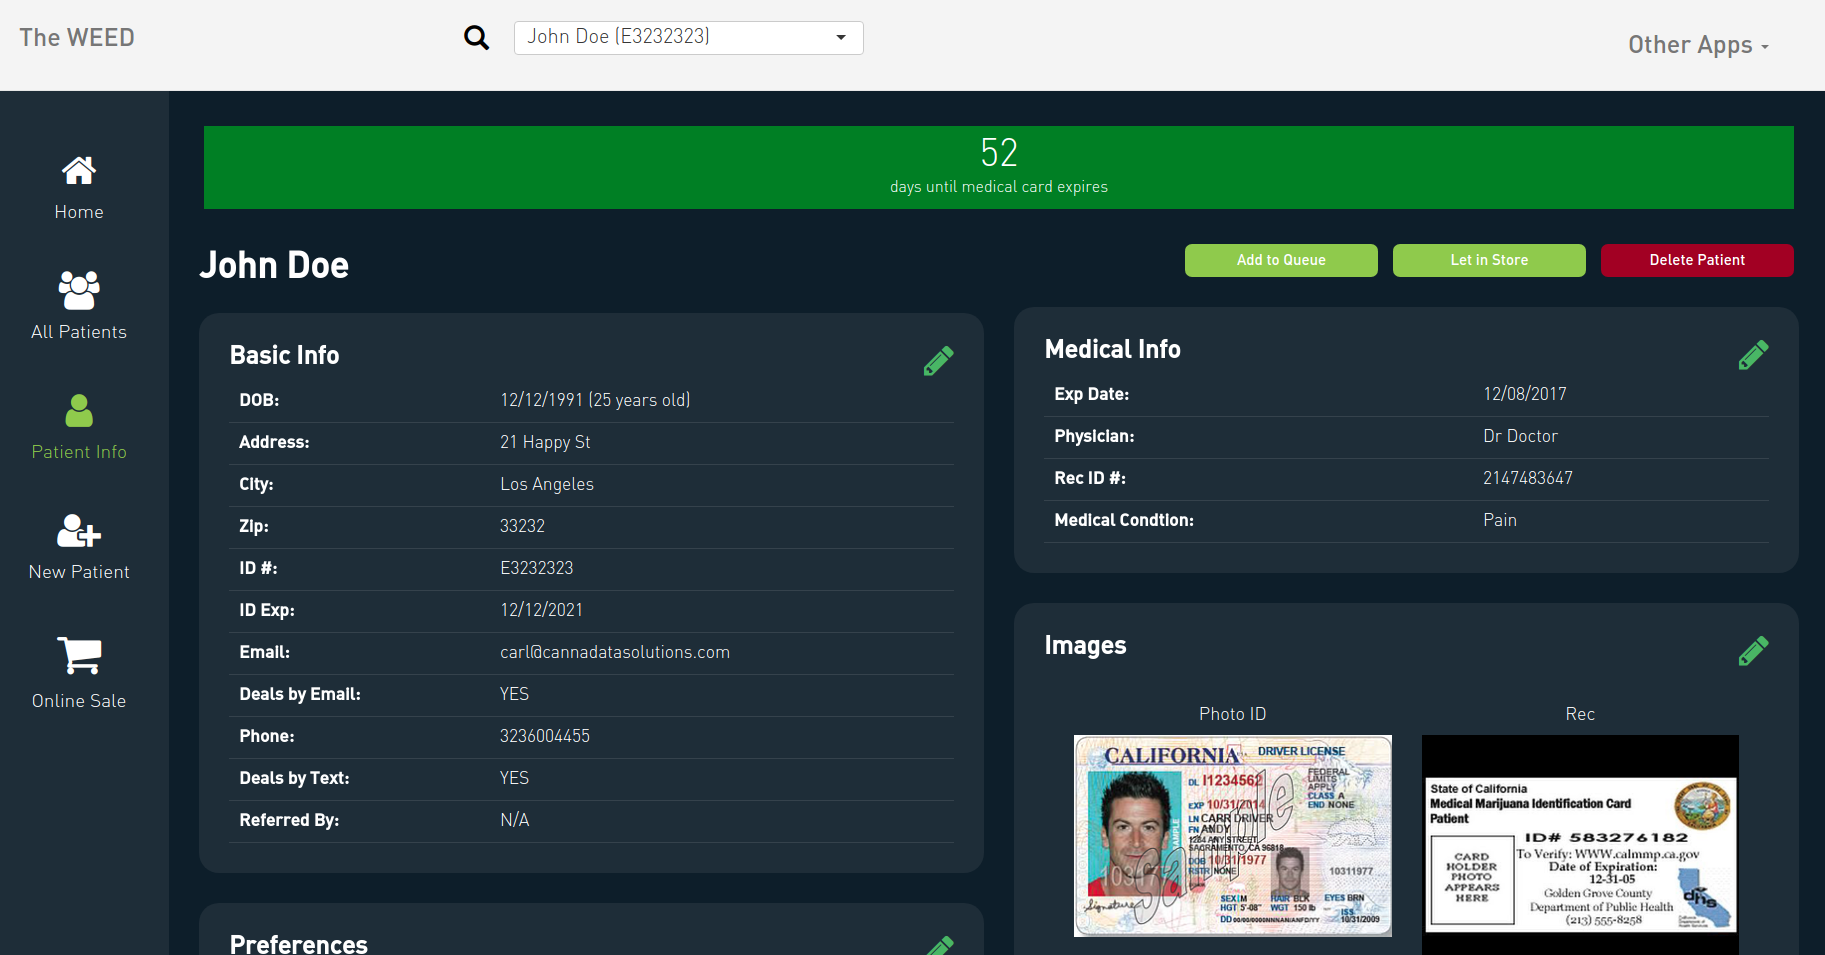
\includegraphics{images/patientInfo.png}
\caption{Returning Patient Info}
\end{figure}

The patient info page provides basic data about the patient, as well as
their medical info. The box at the top displays the number of days left
until the patient's medical card expires. When expired, the box is red.

\begin{figure}
\centering
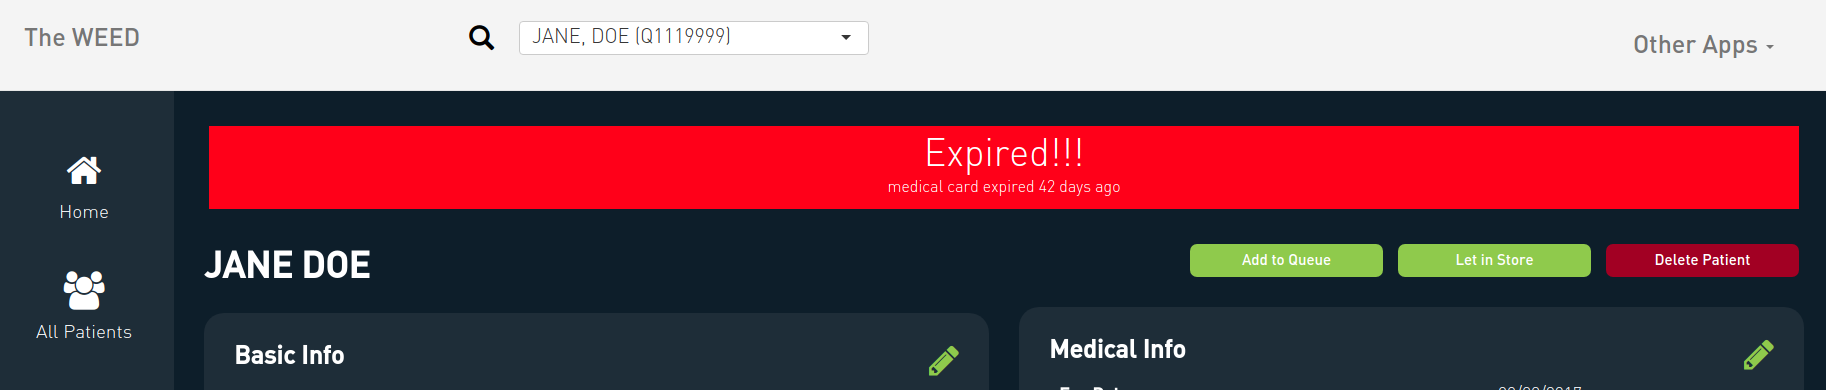
\includegraphics{images/expired.png}
\caption{Expired Patient}
\end{figure}

There are two graphs, one displaying the number of reward points the
patient has accumulated, and a pie chart representing the product types
from the patient's purchase history.

\begin{figure}
\centering
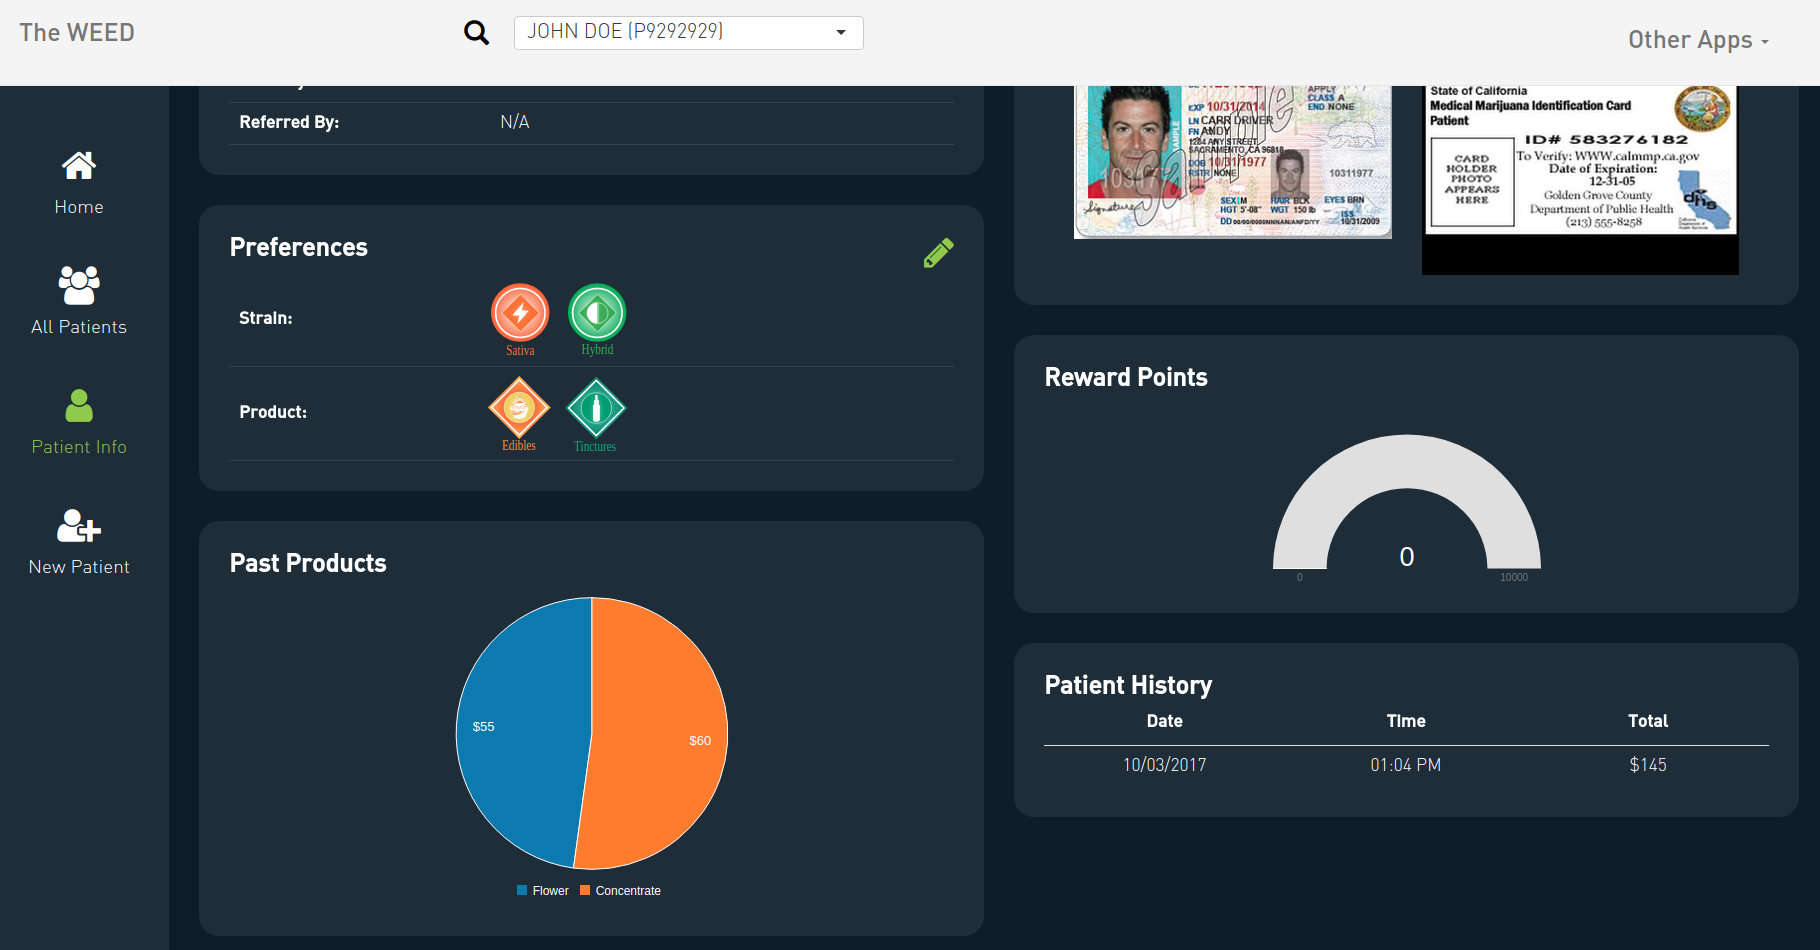
\includegraphics{images/patientInfo2.png}
\caption{Patient Data}
\end{figure}

You can view details of past transactions by selecting a row from the
patient history table.

\begin{figure}
\centering
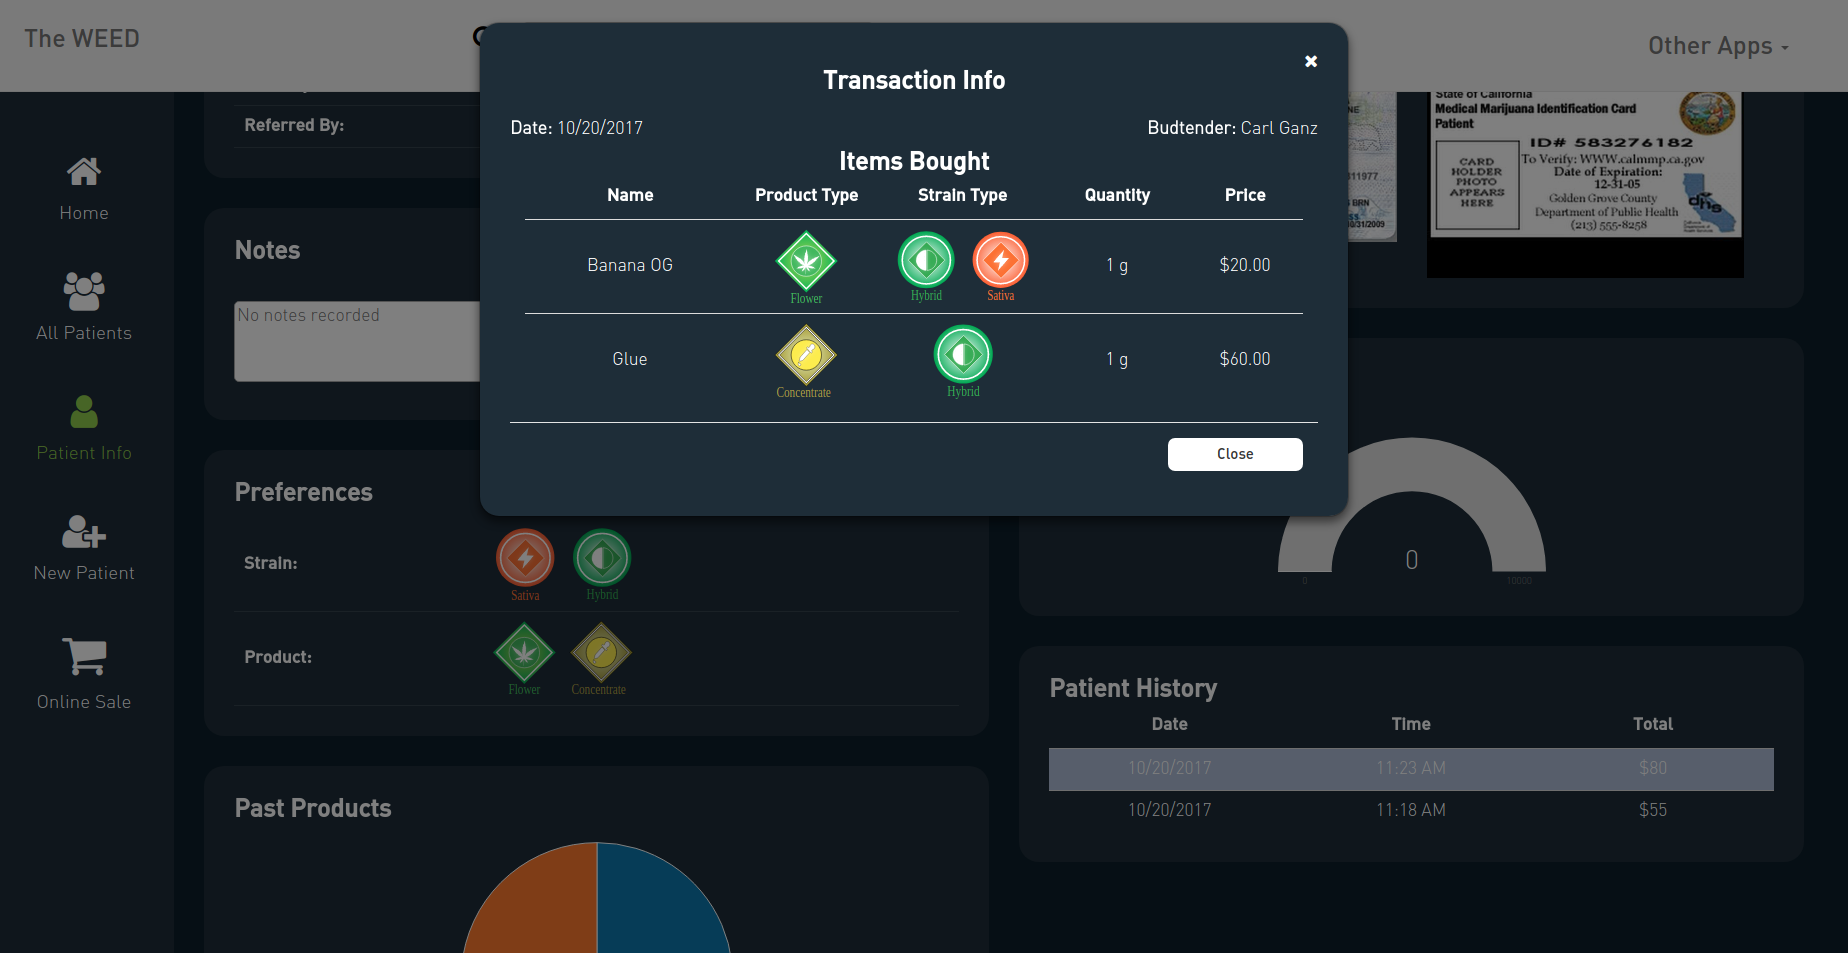
\includegraphics{images/pastTransaction.png}
\caption{Past Transaction}
\end{figure}

For patients with expired medical cards, the patient info page lets you
edit, and update the patients medical info.

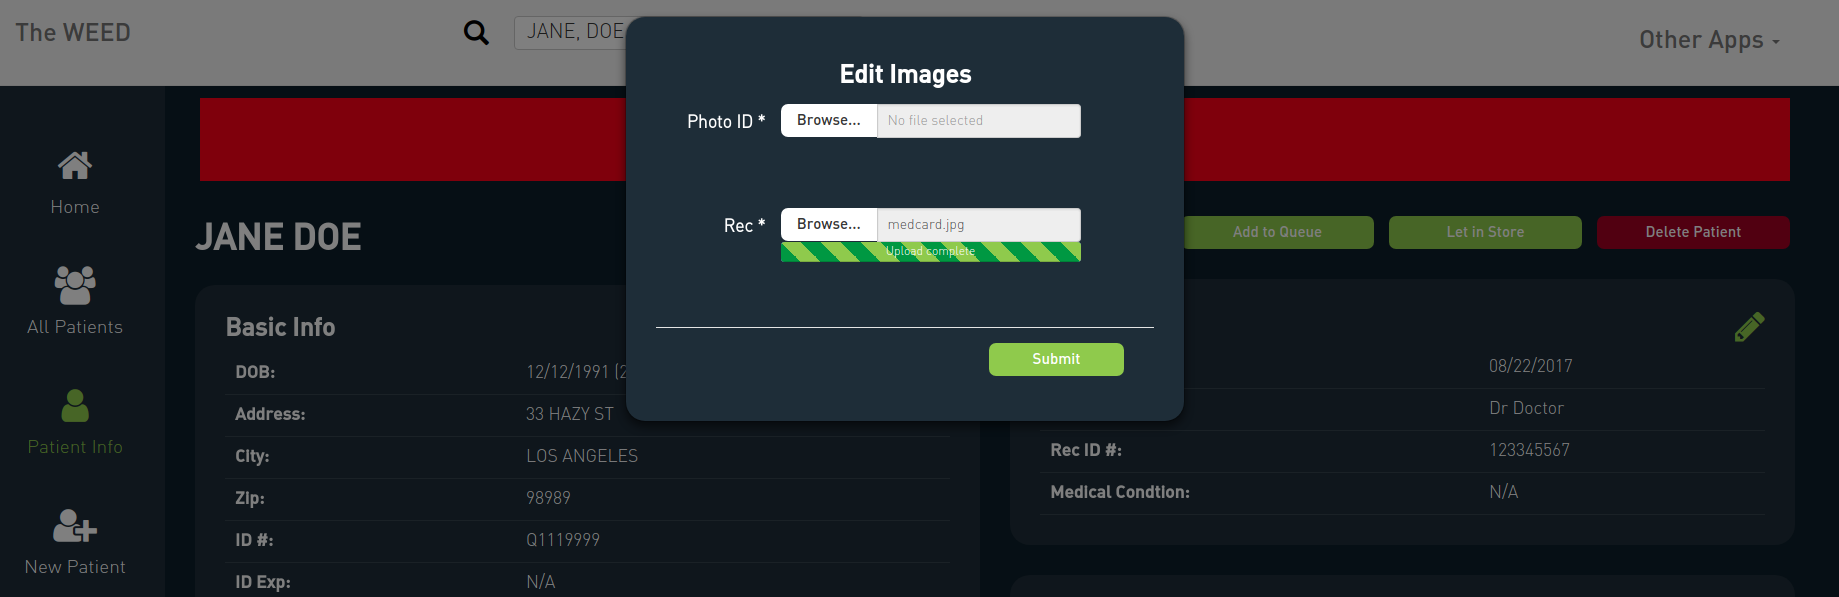
\includegraphics{images/edit1.png} 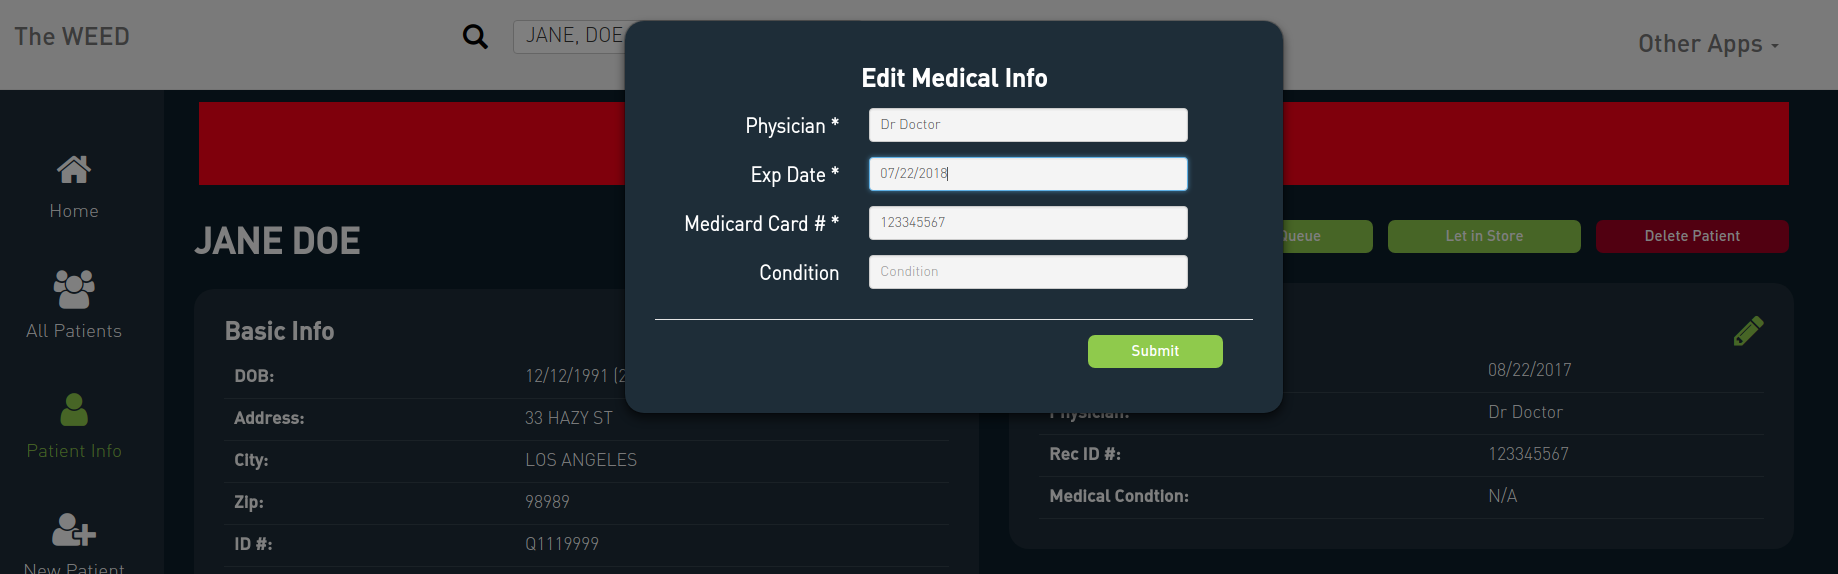
\includegraphics{images/edit2.png}

You can also access a patient's info page by either searching for them
in search box at the top, or by selecting them from the All Patients
tab.

\begin{figure}
\centering
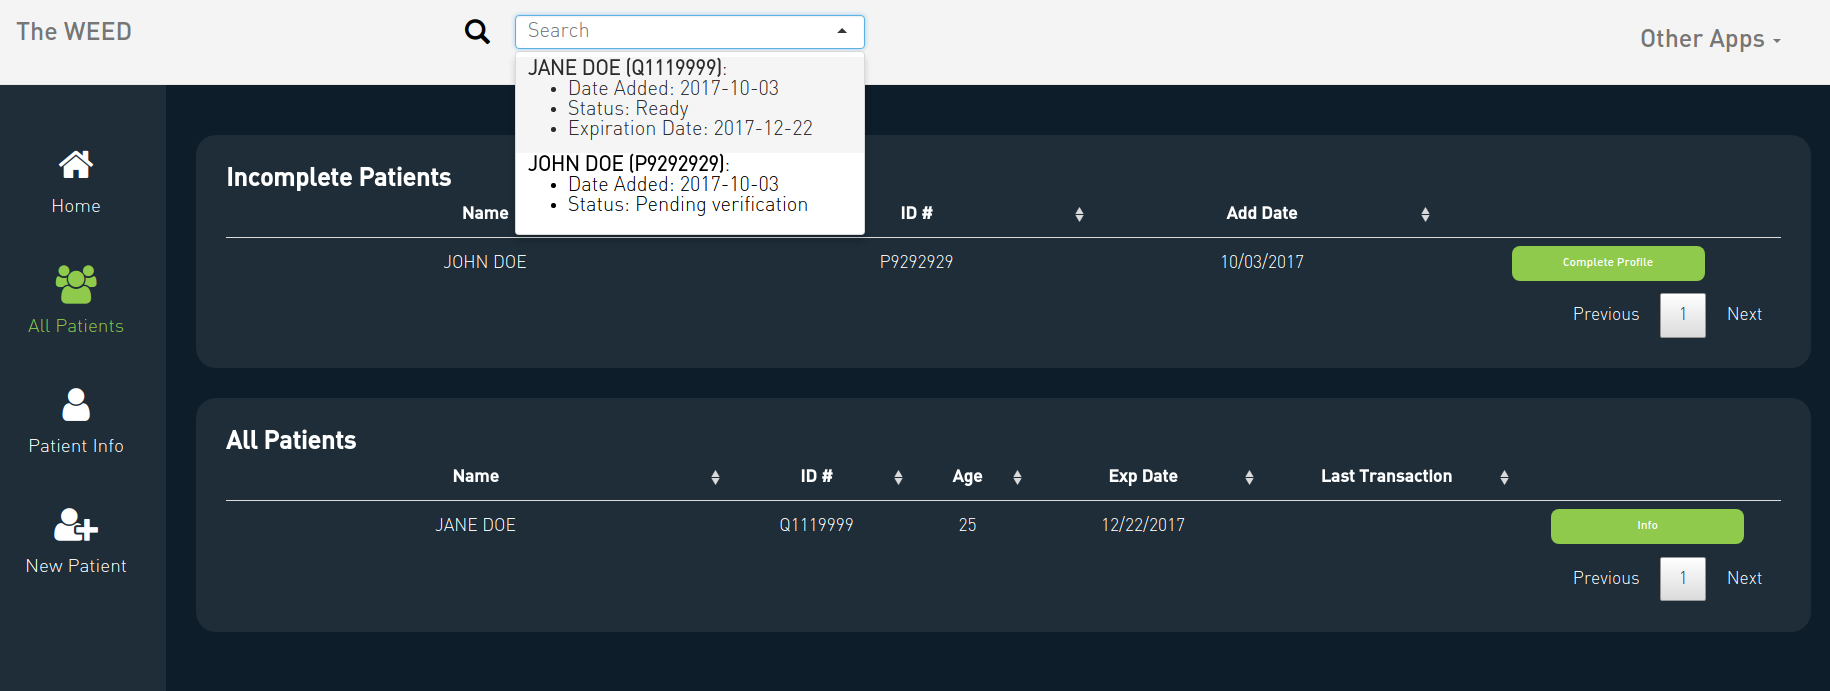
\includegraphics{images/allPatients.png}
\caption{All Patient Table}
\end{figure}

The All Patients tab also allows you to view, which patient profiles are
incomplete, and which registered patients have expired medical cards.

\subsection{Queue}\label{queue}

The homepage of the Frontdesk app keeps track of who is currently in the
store, and who is currently in line to get in the store (queue). These
tables make it easy to see who is next in line, and how long people have
been waiting.

\begin{figure}
\centering
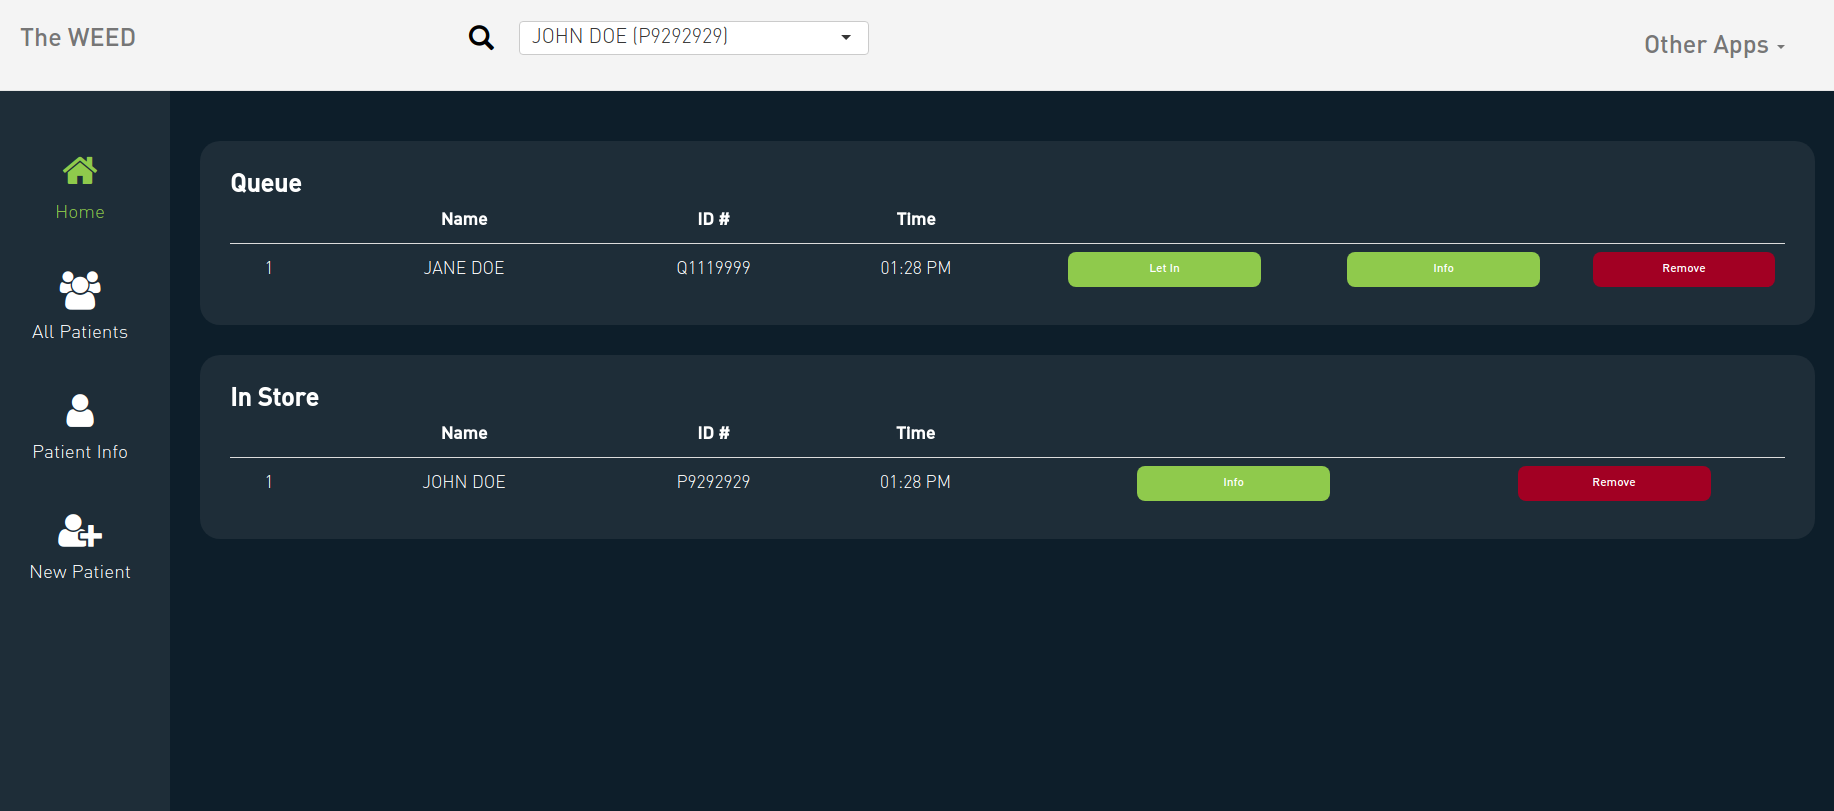
\includegraphics{images/queue.png}
\caption{Queue}
\end{figure}

\section{New Patients}\label{new-patients}

For new patients, when their ID is scanned a message will appear
indicating that the patient is new. The budtender has the option to add
the new patient which initiates the patient sign-up process.

\begin{figure}
\centering
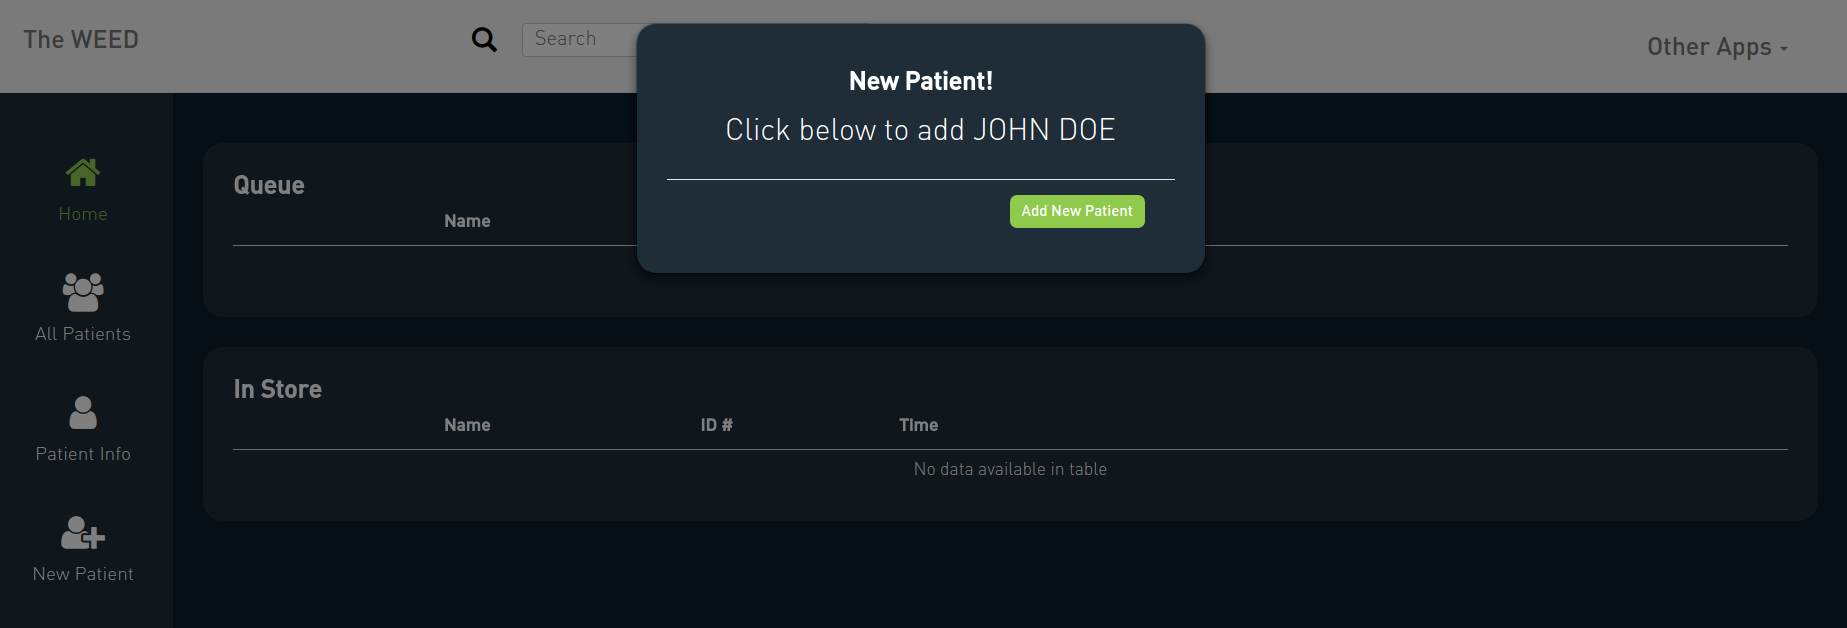
\includegraphics{images/addnew.png}
\caption{Add New Patient Screen}
\end{figure}

When the patient's ID is first scanned, the information from their ID is
automatically added. The budtender uploads the patient's documents, and
enter a small amount of information from the patient's medical card,
specifically the name of their doctor, the expiration date, and the
medical card ID number.

\begin{figure}
\centering
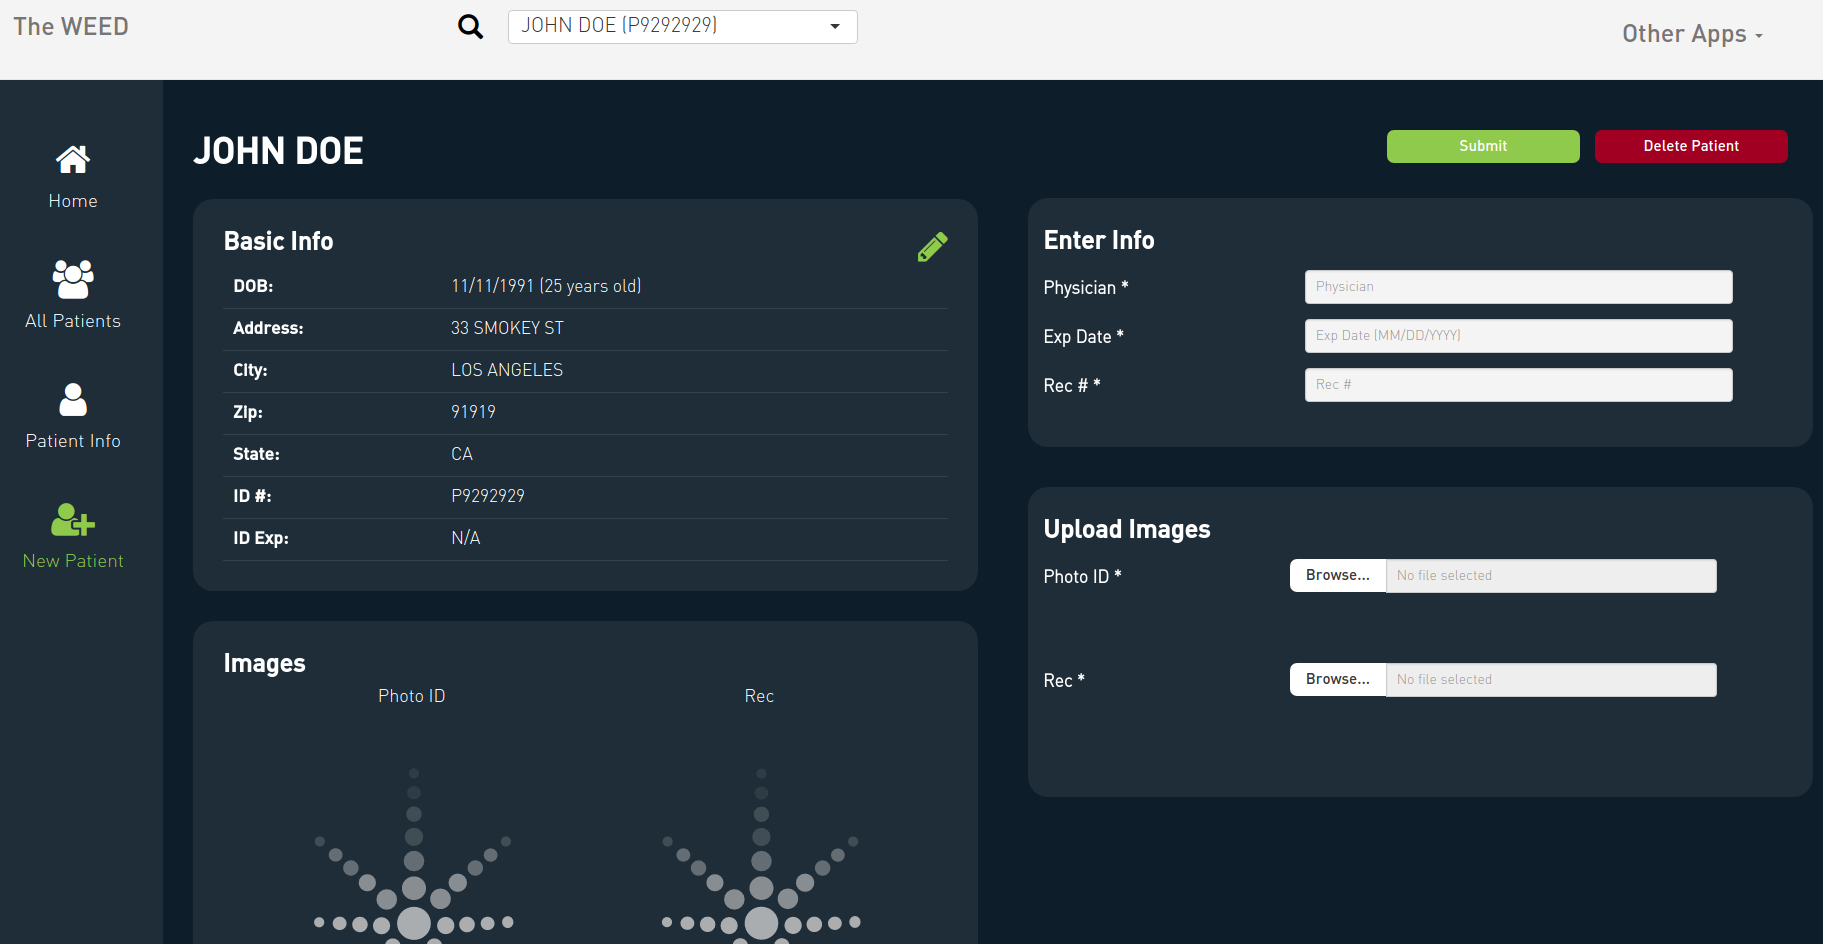
\includegraphics{images/NewPatient.png}
\caption{Empty New Patient Form}
\end{figure}

\begin{figure}
\centering
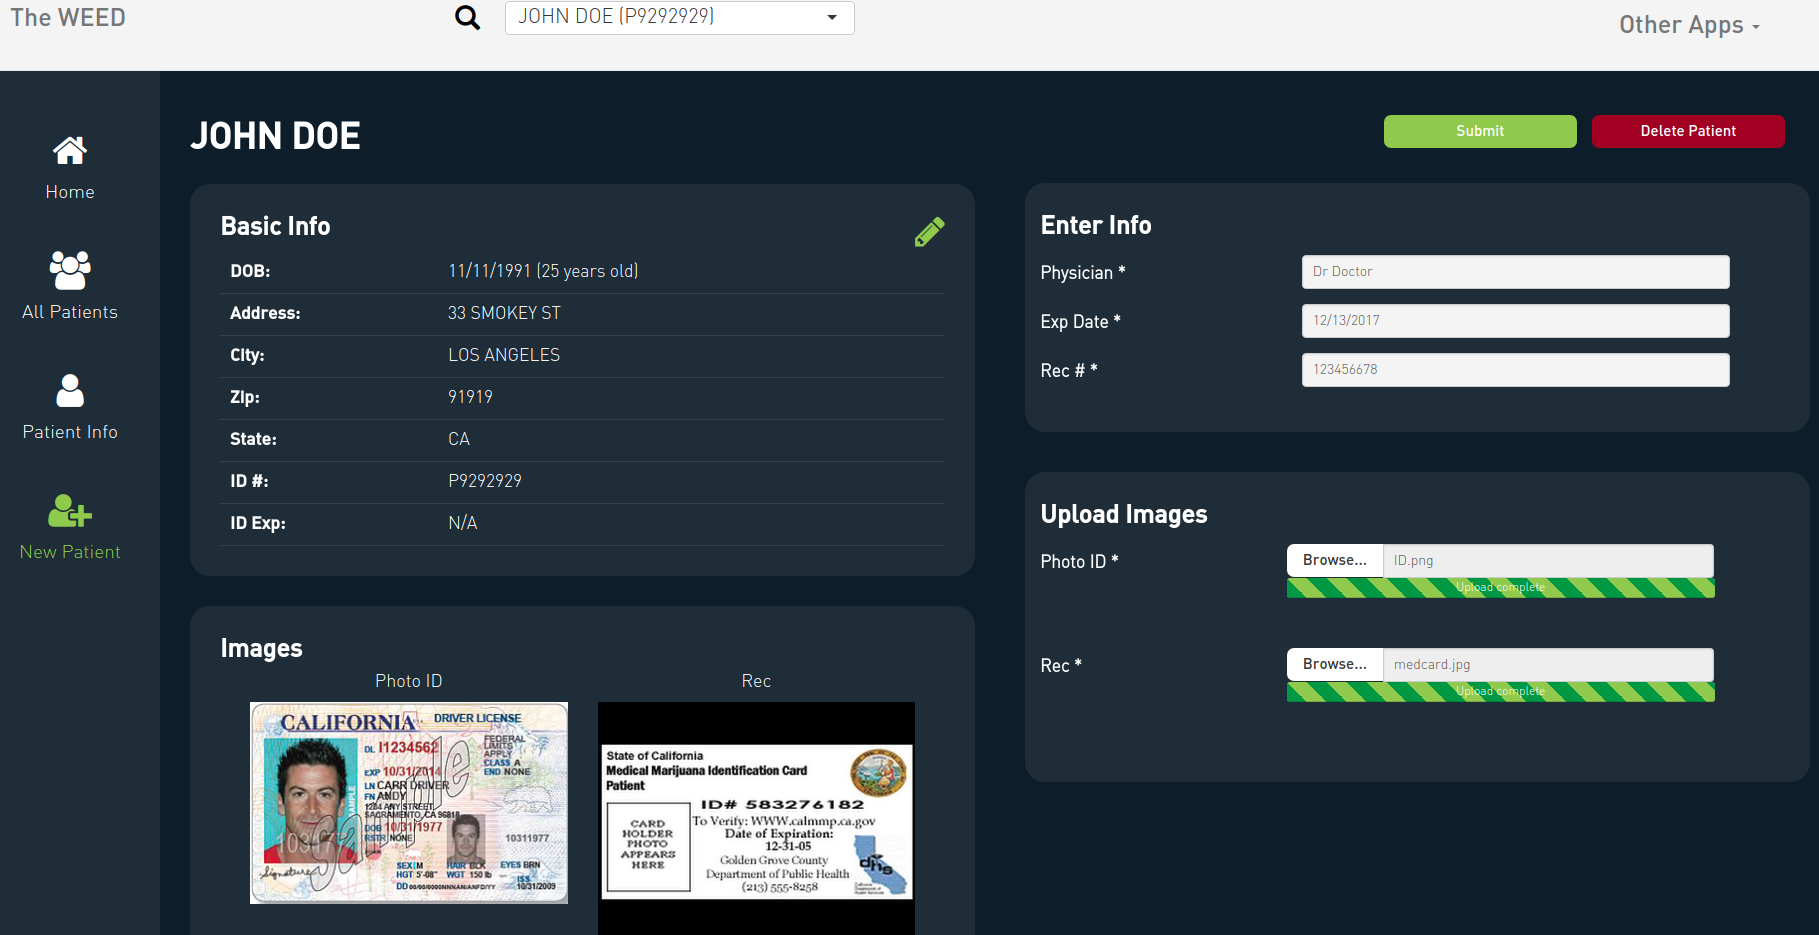
\includegraphics{images/newPatient2.png}
\caption{Completed New Patient Form}
\end{figure}

While the budtender enters this information, the patient is presented
with an iPad (or other tablet or computer) where they enter their
information into the Signup application discussed below.

\subsection{Signup}\label{signup}

The Signup application works in conjunction with the Frontdesk app to
let new patients quickly join a dispensary. When a new patient's ID is
scanned they are added to the database, but their profile is incomplete.
The budtender must input the patient's medical information (discussed
above), and the patient must complete the signup form (and sign the
patient agreement), before they can enter the store. The first page of
the signup form contains an input where the budtender can select the
incomplete profile of the new patient. If only one patient is signing up
they will automatically be selected.

Once the incomplete profile is selected the budtender would hand the
iPad over to the new patient who would fill out the rest of the form.
The first page of the signup form is automatically filled in based on
the information on the patient's driver's license.

\begin{figure}
\centering
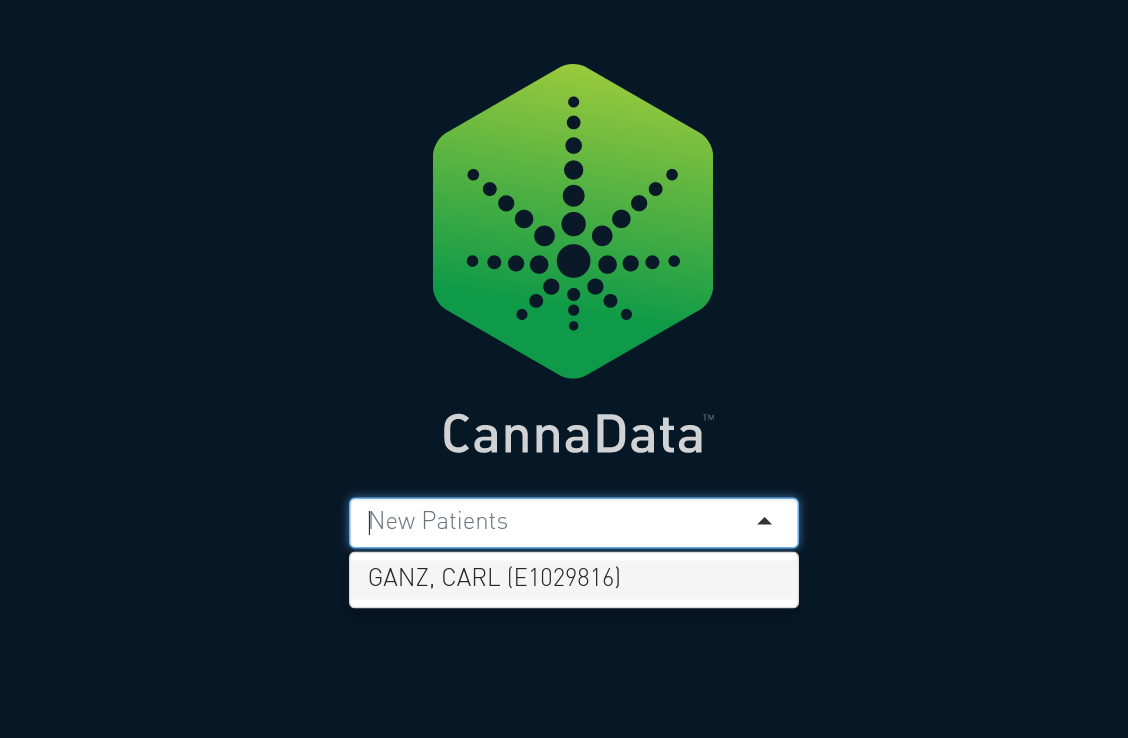
\includegraphics{images/S1.png}
\caption{Autofilled Basic Info}
\end{figure}

There are four additional pages where the patient fills in their contact
info, and preferences.

\begin{figure}
\centering
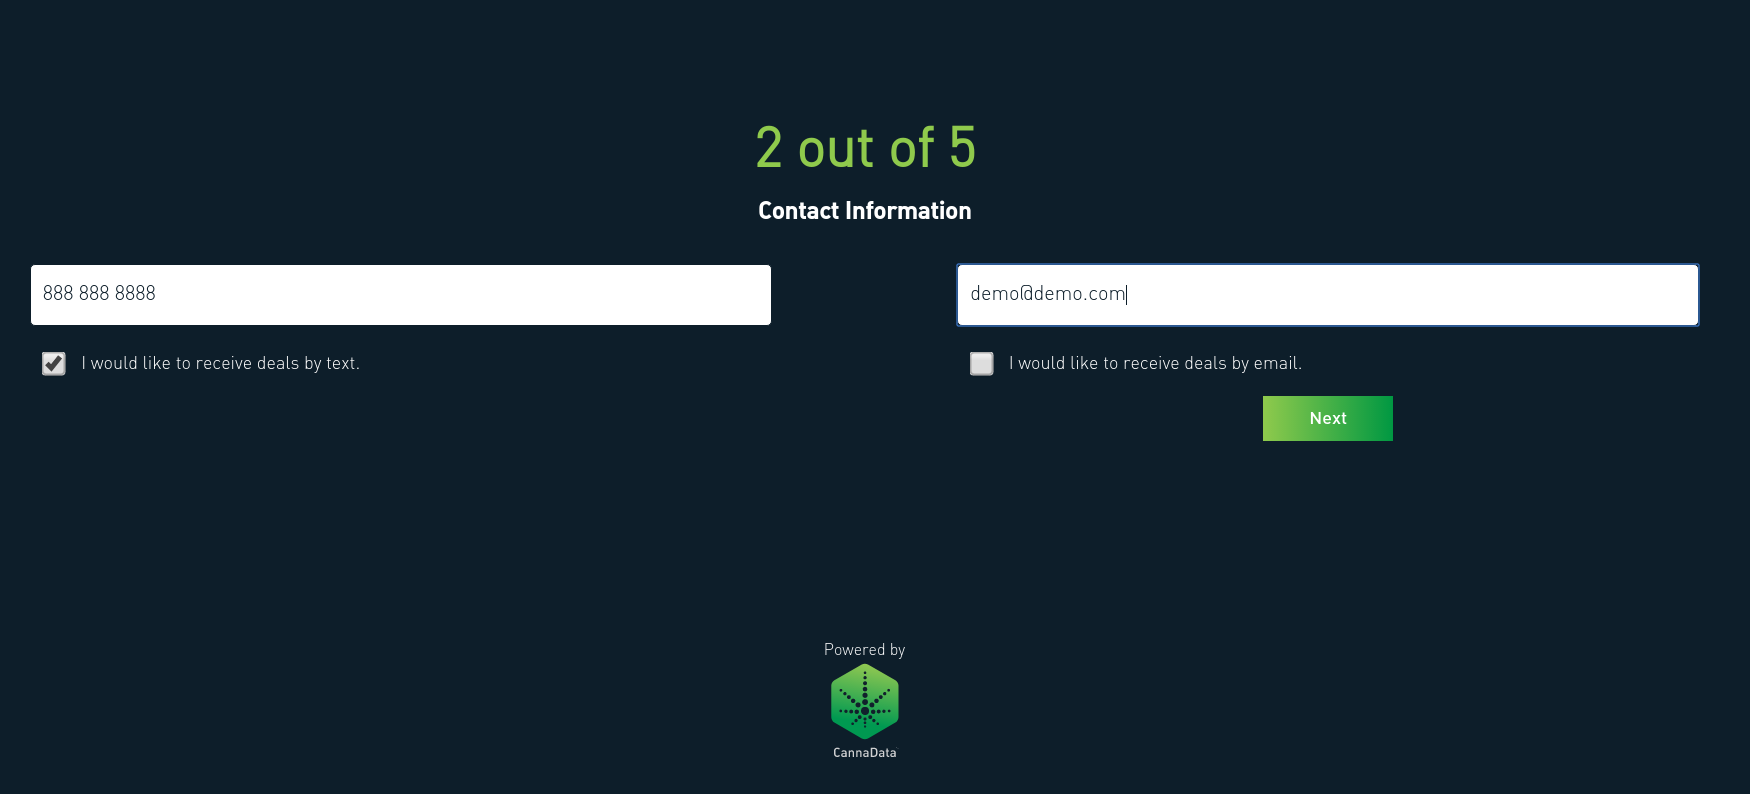
\includegraphics{images/S4.png}
\caption{Contact Info}
\end{figure}

\begin{figure}
\centering
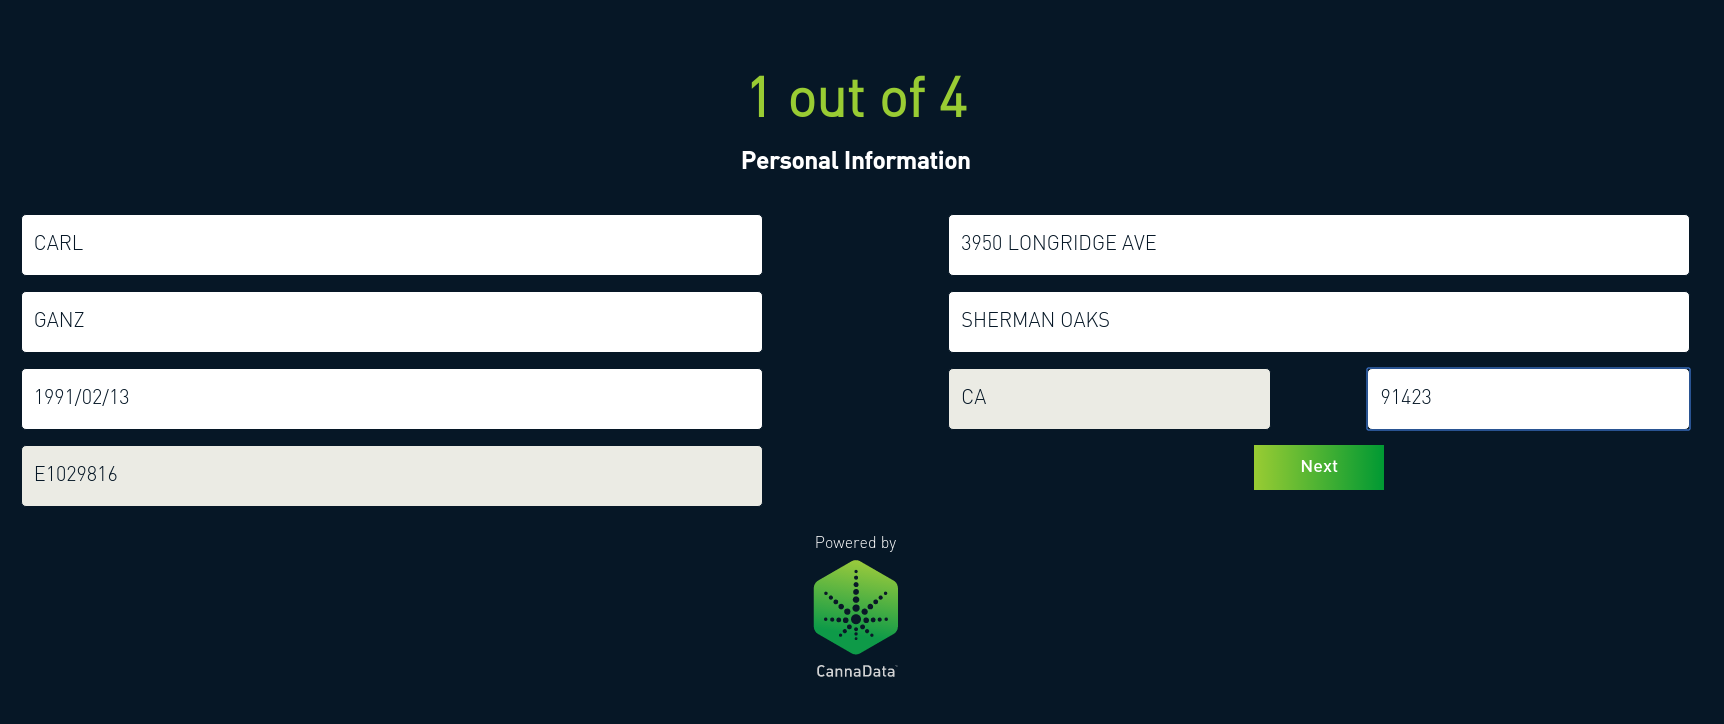
\includegraphics{images/S2.png}
\caption{Preference Info}
\end{figure}

\begin{figure}
\centering
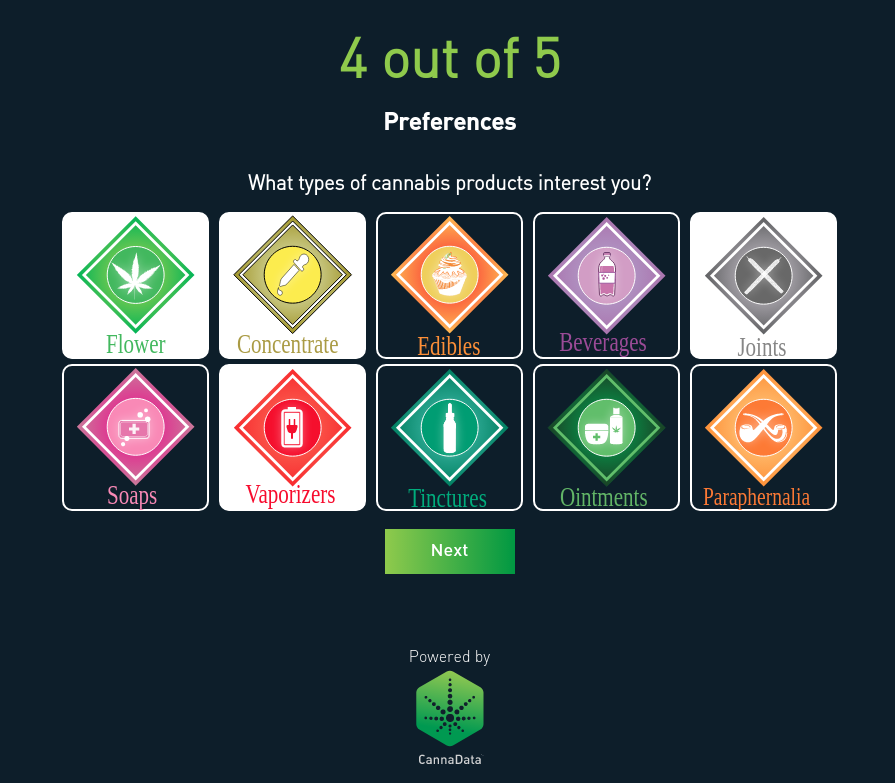
\includegraphics{images/S3.png}
\caption{Preference Info}
\end{figure}

\begin{figure}
\centering
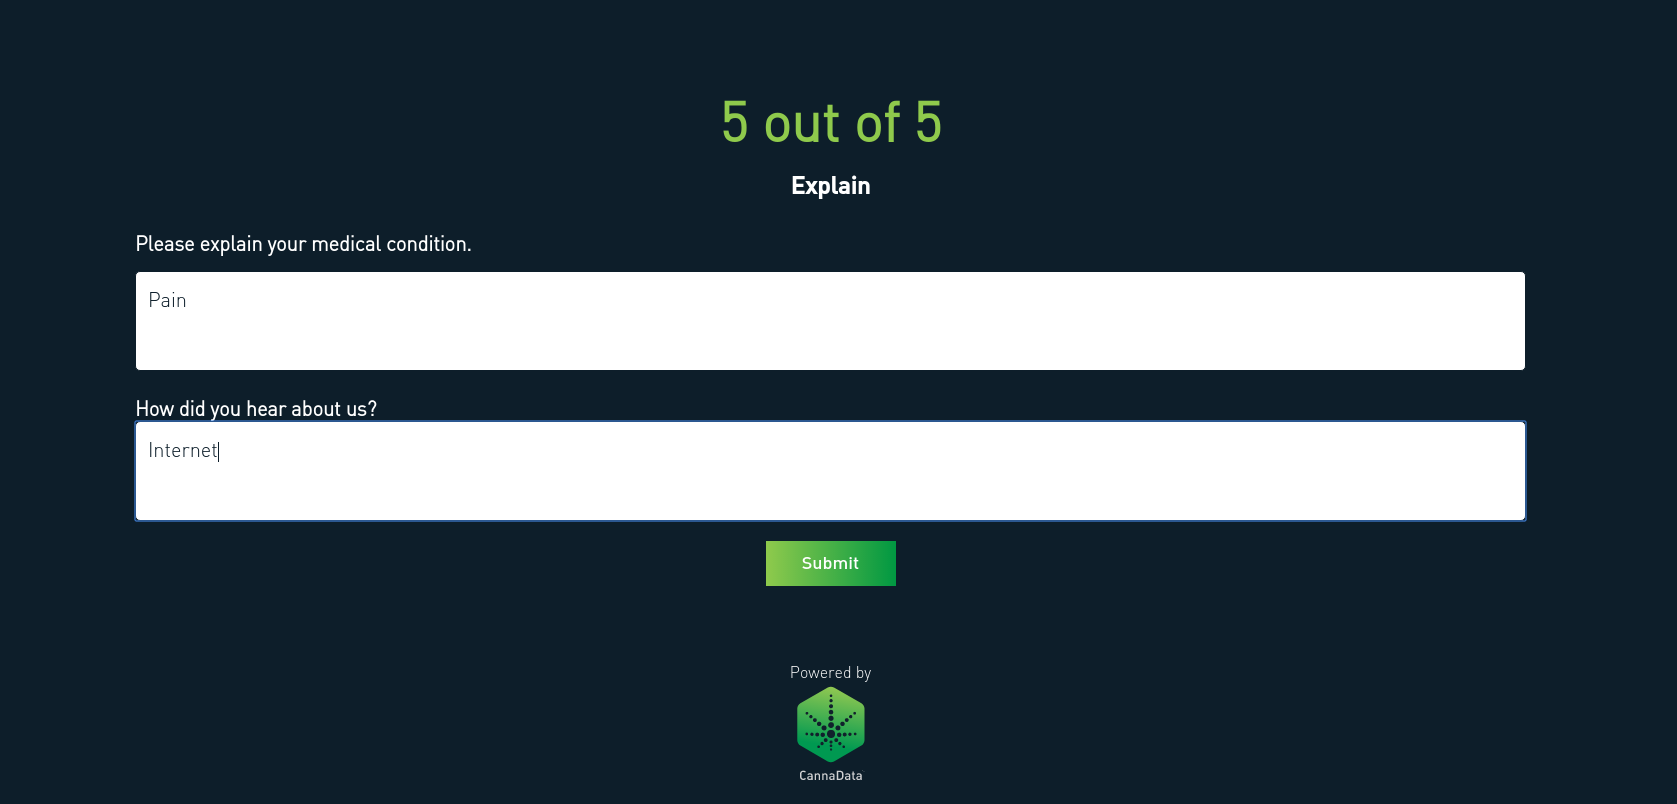
\includegraphics{images/S5.png}
\caption{Other Info}
\end{figure}

After the patient completes the form they are automatically sent to
DocuSign where they digitally sign the new patient agreement contract.
This makes the signup process completely paperless.

\chapter{Inventory}\label{inventory}

The Inventory Management application provides facilities for:

\begin{itemize}
\item
  Adding new inventory and new wholesalers
\item
  Viewing the performance of past products and wholesalers
\item
  Checking quantities of current stock
\item
  Updating/editing information about existing products
\item
  Print labels/barcodes for inventory
\end{itemize}

\section{New Inventory}\label{new-inventory}

The new inventory page allows you to enter new shipments of inventory
into your database. Digitally managing inventory doesn't just make it
easier to keep track of products, but it also simplifies the record
keeping process required for taxes, and other regulations.

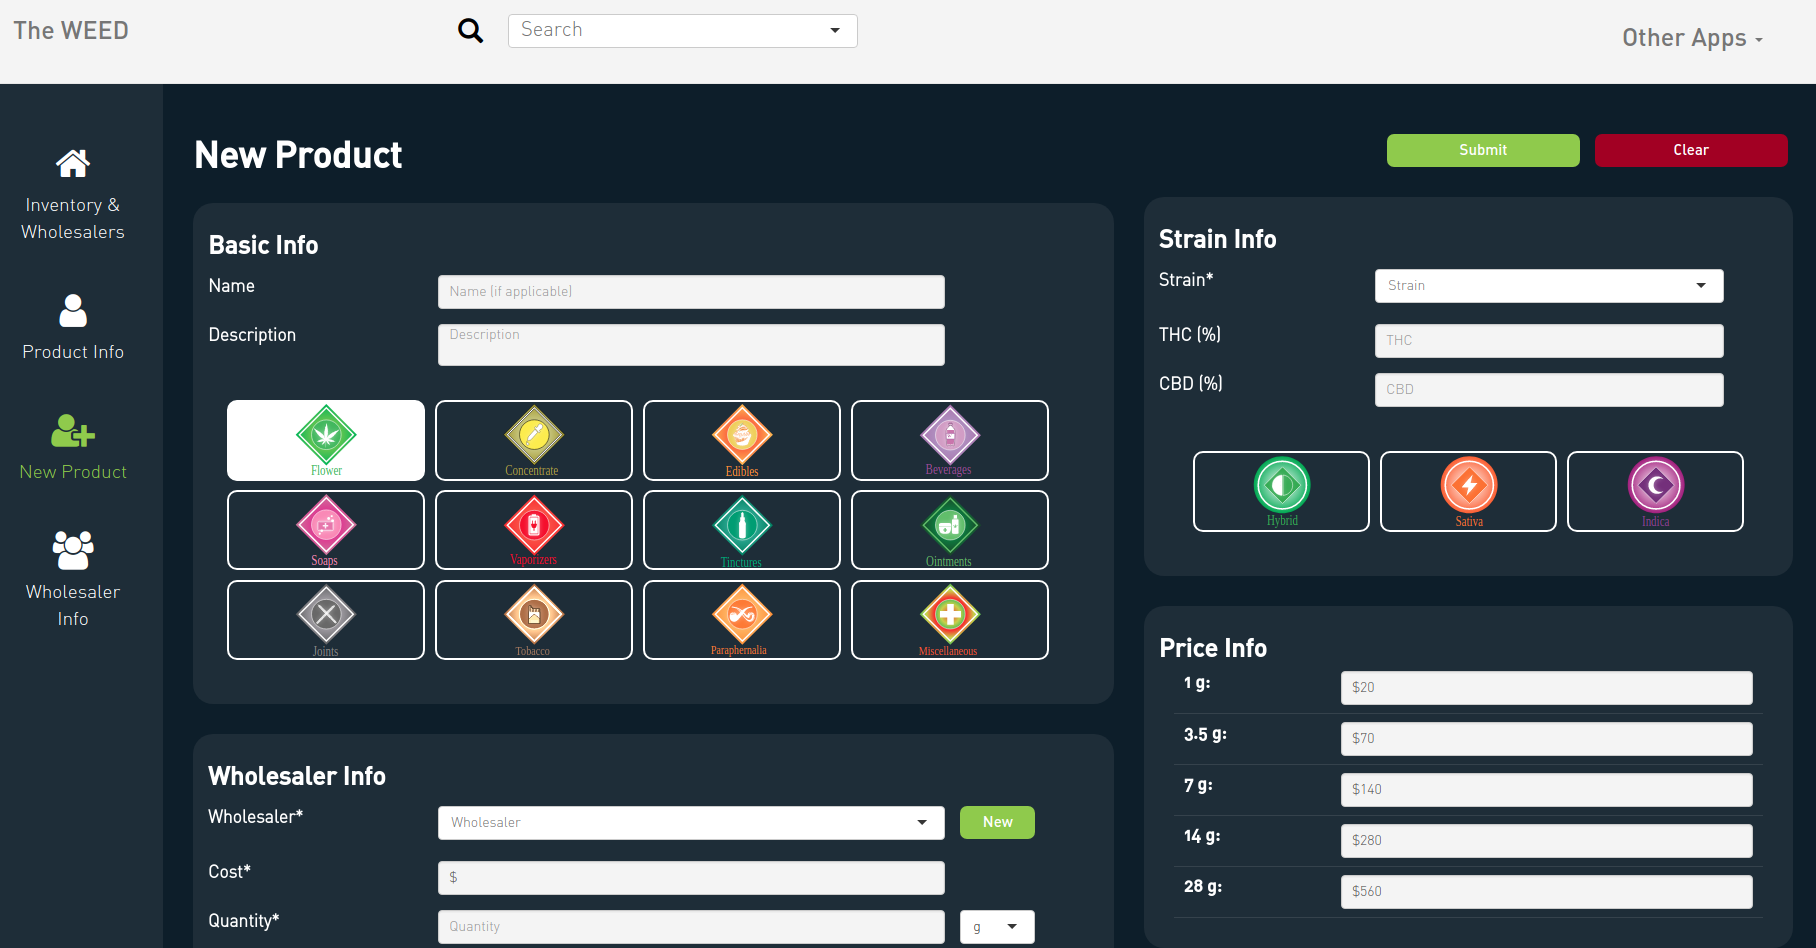
\includegraphics{images/newInv.png} 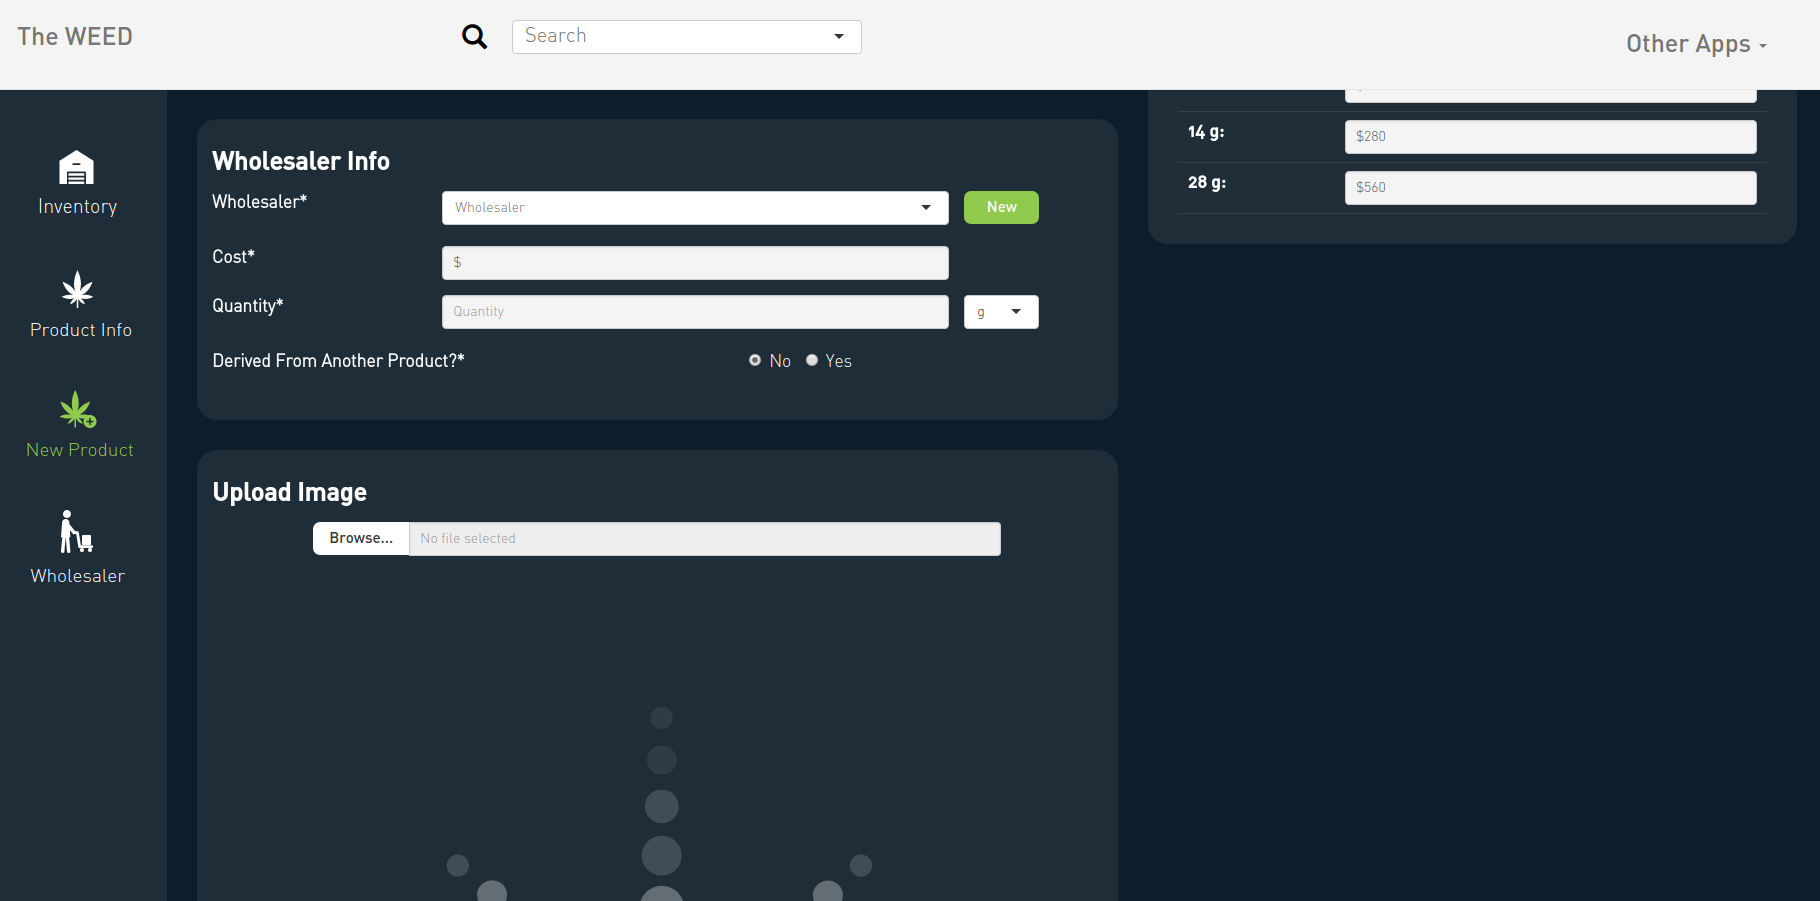
\includegraphics{images/newInv2.png}

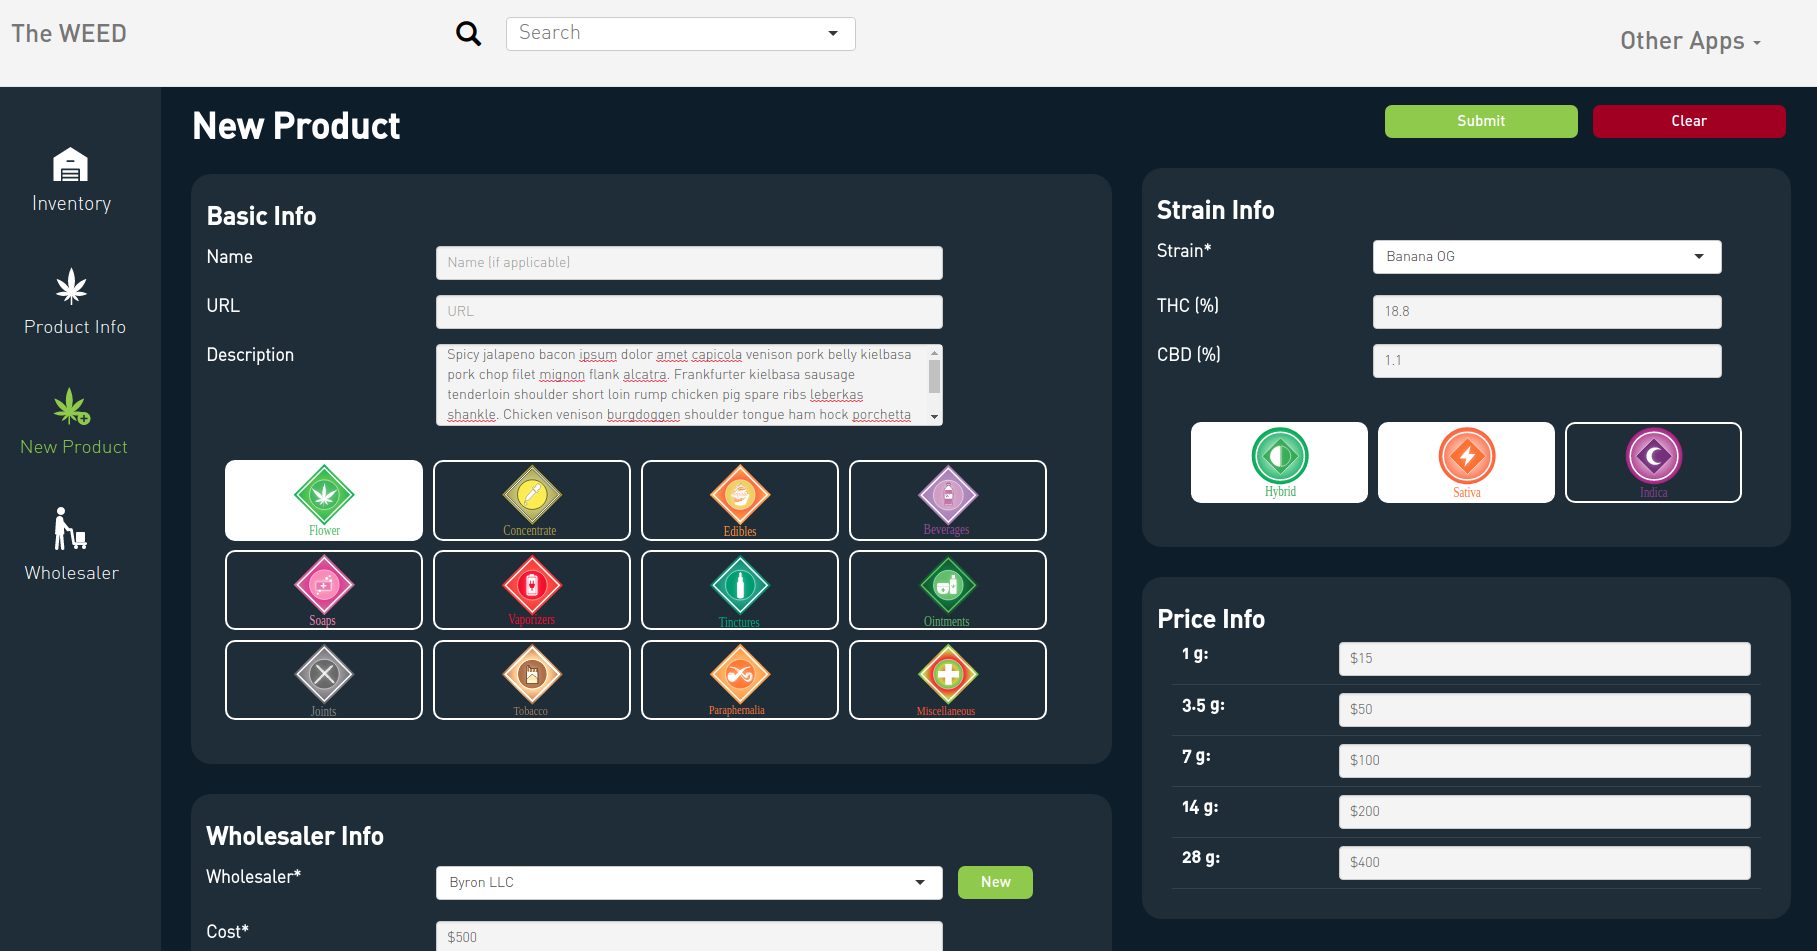
\includegraphics{images/newInv3.png}
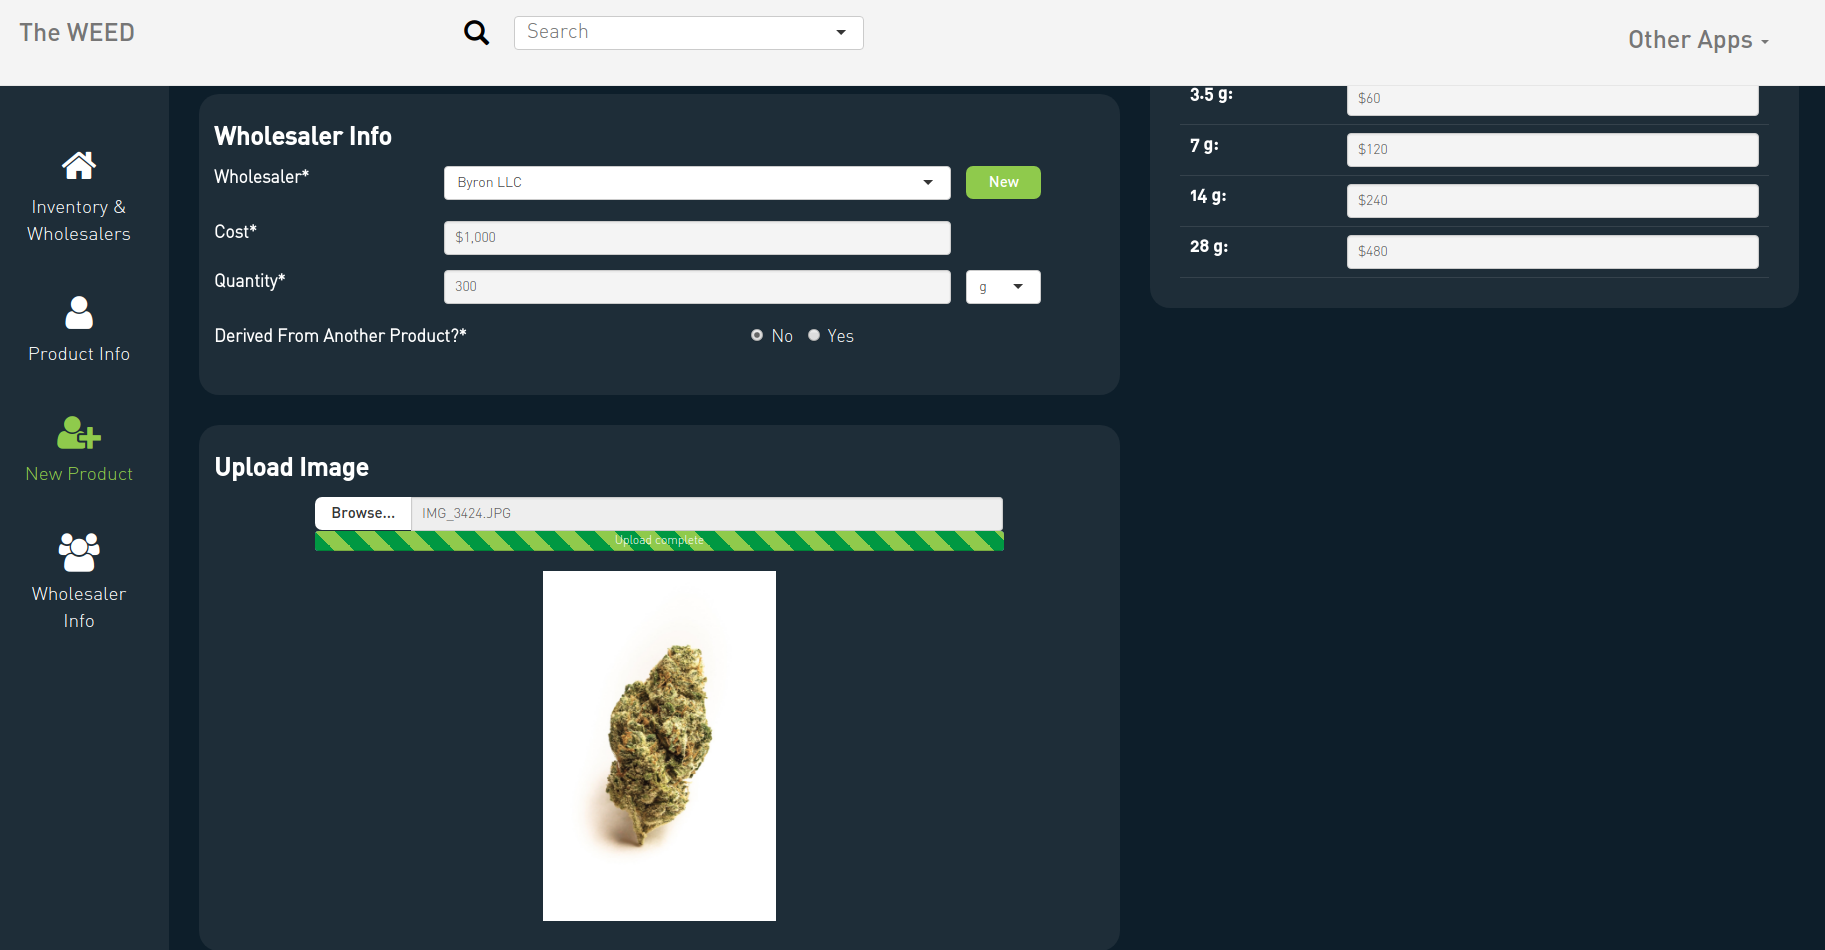
\includegraphics{images/newInv4.png}

There are several required fields in the new inventory form:

\begin{itemize}
\item
  Product Type (i.e.~flower vs concentrate vs edible etc.)
\item
  Strain (No strain is an option, but must be explicitely selected)
\item
  Wholesaler
\item
  Wholesale price
\item
  Quantity
\item
  Price
\end{itemize}

There are also several optional inputs, and inputs that are only
required sometimes:

\begin{itemize}
\item
  Product Name (required if no strain selected)
\item
  Specific Product Type (i.e.~is concentrate wax/shatter/kief? is edible
  cookie/brownie/cheeseburger?)
\item
  Description
\item
  THC \& CBD levels
\item
  Whether product is Indica/Sativa/Hybrid
\item
  Image
\item
  Source product and quantity (i.e.~if you take 50 grams of Banana OG
  and make 75 joints, when you enter the 75 joints you would also want
  to remove the 50 grams of Banana OG that the joints are derived from)
\end{itemize}

\subsection{Pricing}\label{pricing}

The price input contains default values based on the product type.
Whenever a value in the price input is updated, the rows below the
changed value, representing the price for larger quantities, are updated
to be consistent with the new value. For example, the default price for
concentrates is \$30 per half gram. This rate is used for higher
quantities so 1 gram is \$30*2=\$60, two grams is \$30*4=\$120, etc. We
can update the price for two grams to \$100, which translates to \$50
per gram. Now all quantities above two grams are priced at the \$50 per
gram rate, while all quantities below two grams retain the \$30 per half
gram (\$60 per gram) rate.

\begin{figure}
\centering
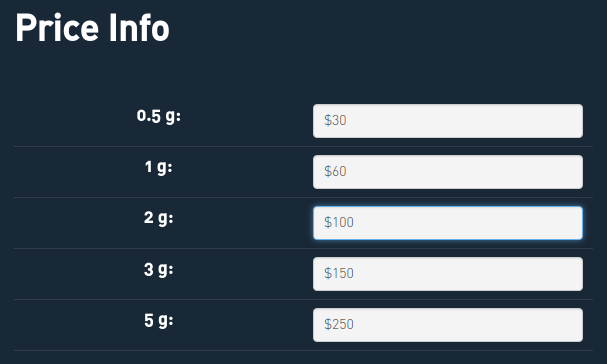
\includegraphics{images/I3.png}
\caption{Price Input with 2 g level manually set to \$100}
\end{figure}

\section{Past Products}\label{past-products}

Details about existing and past products are easily accessible. You can
search for any inventory or wholesaler in the search box at the top. You
can also view tables containing current inventory, old inventory, and
wholesalers on the main page.

\begin{figure}
\centering
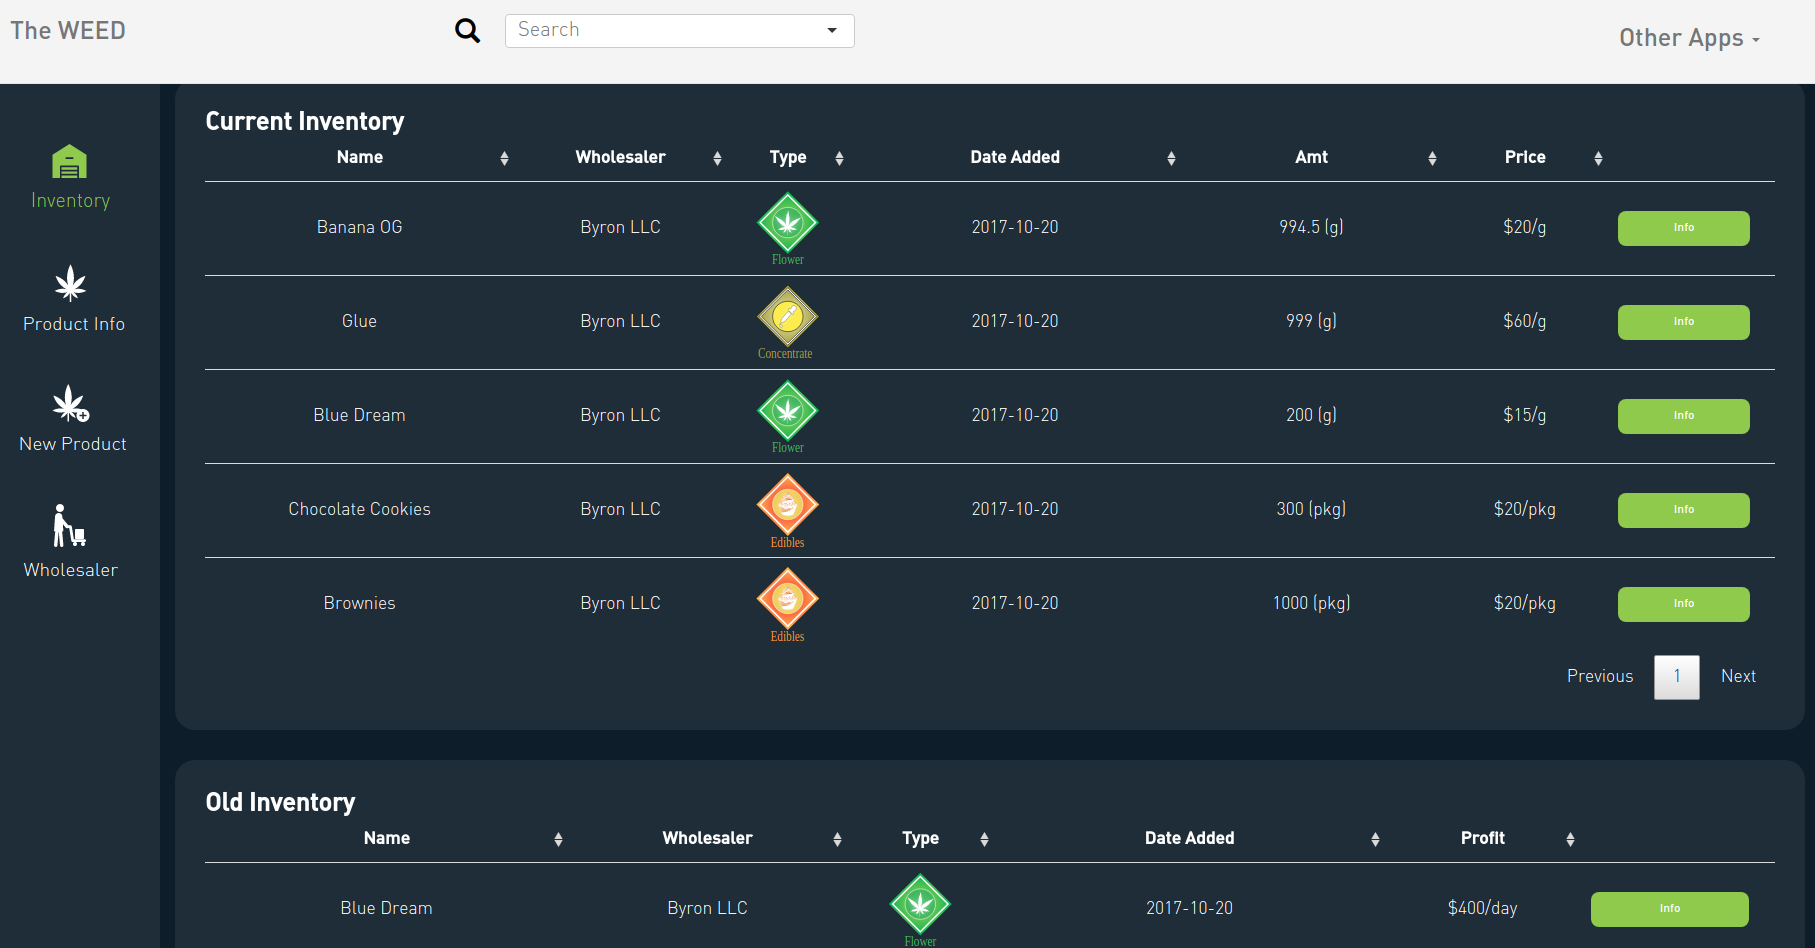
\includegraphics{images/inventory.png}
\caption{Current Inventory Table}
\end{figure}

\begin{figure}
\centering
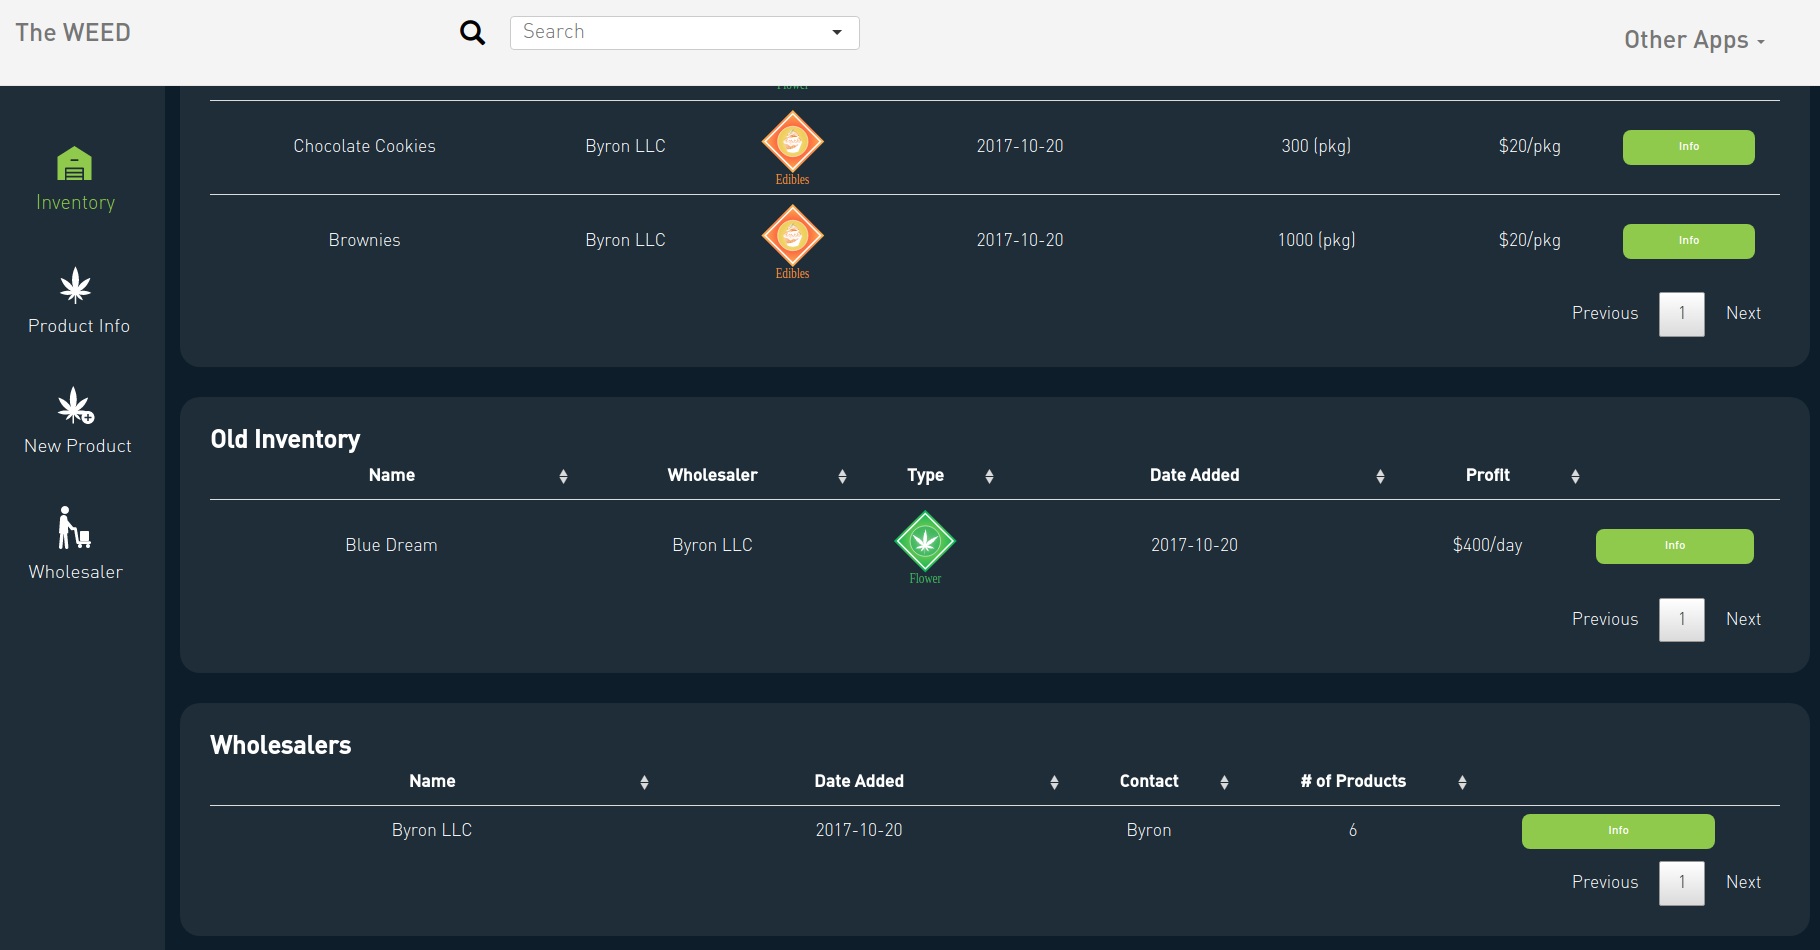
\includegraphics{images/inventory2.png}
\caption{Old Inventory and Wholesalers}
\end{figure}

When you select an item you are taken to the product information page.
This includes a variety of tables regarding the specific product with
the option to edit. Buttons at the top allow to quickly add more
inventory and print barcodes for the product.

\begin{figure}
\centering
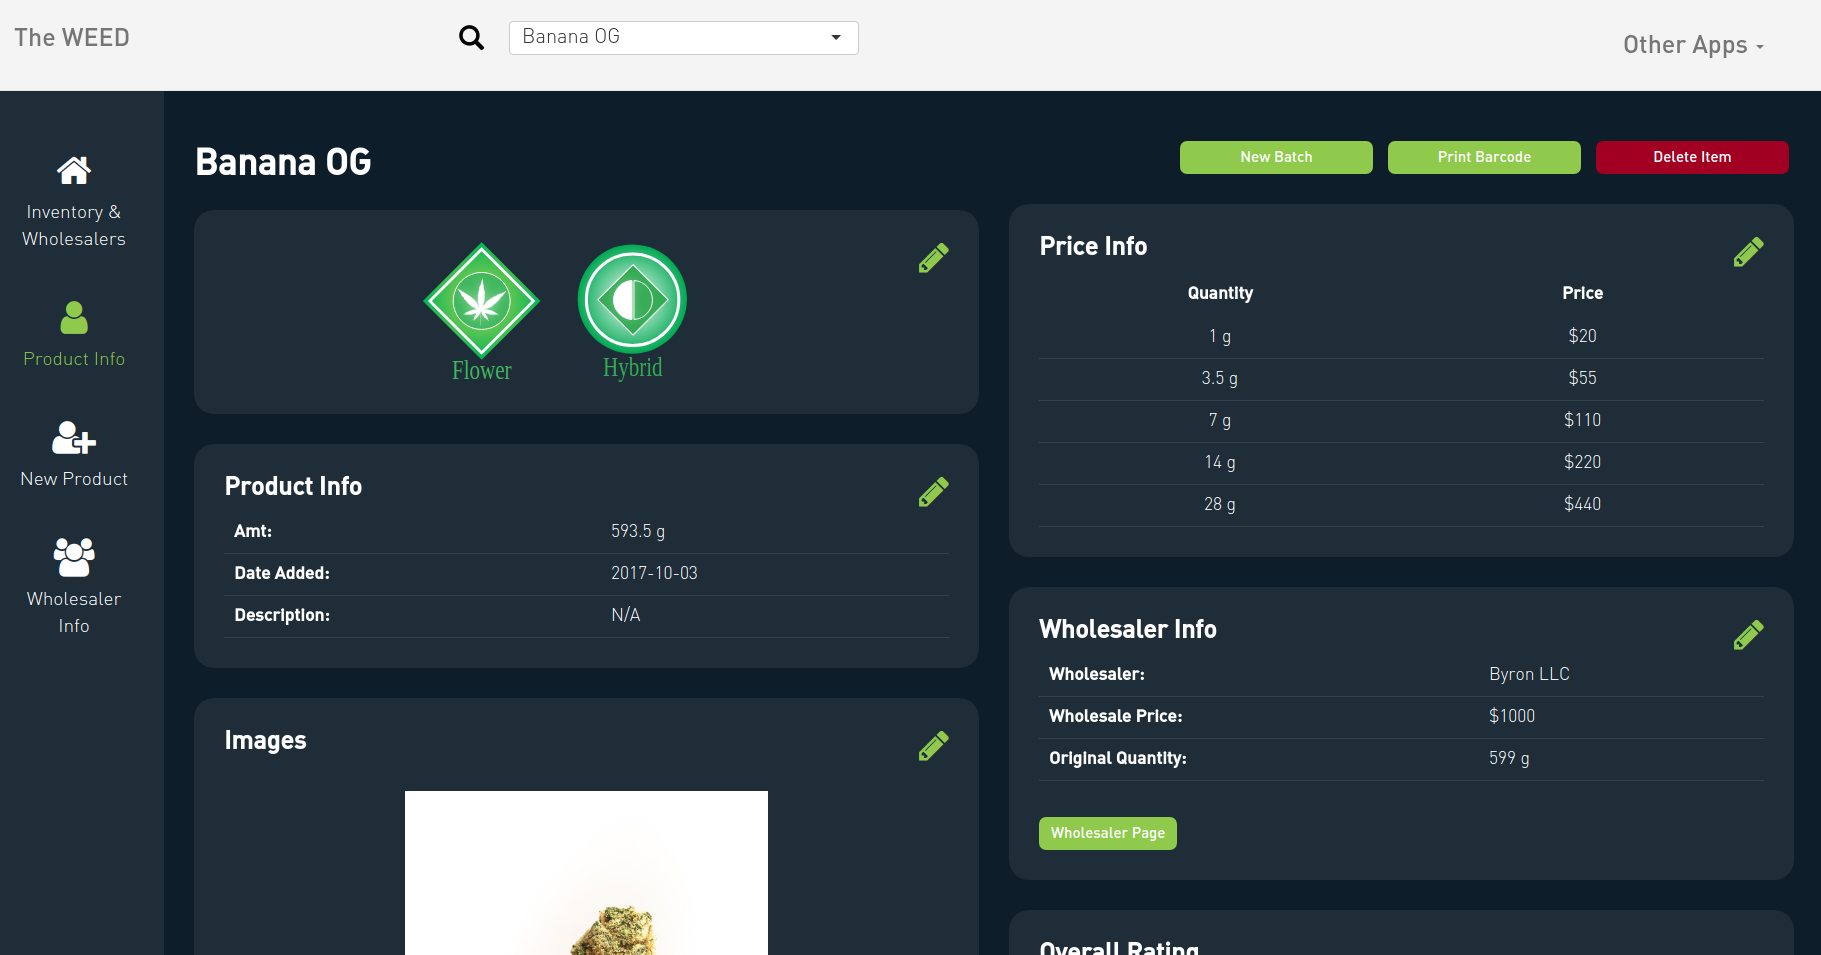
\includegraphics{images/productInfo.png}
\caption{Current Inventory Table}
\end{figure}

Basic analytics are provided so you can quickly see how the product is
performing. Daily sales are charted, and average daily profit is rated
against other similar products.

\begin{figure}
\centering
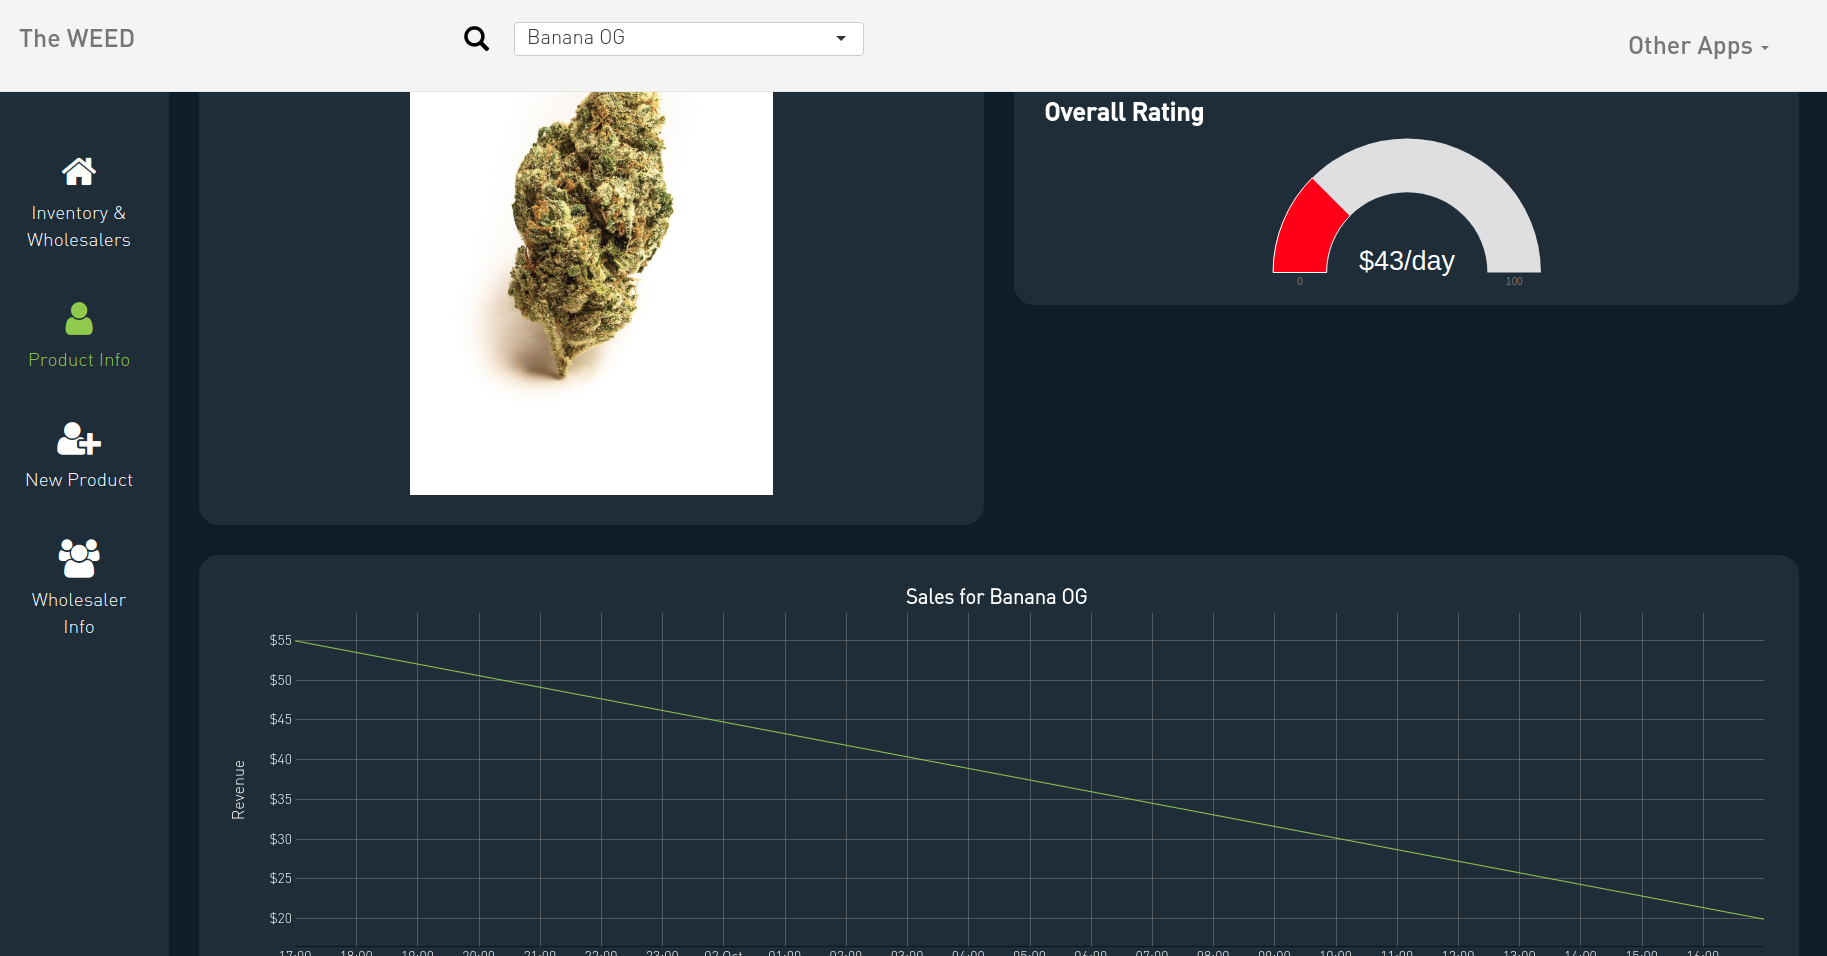
\includegraphics{images/productInfo2.png}
\caption{Current Inventory Table}
\end{figure}

\section{Wholesaler}\label{wholesaler}

You can also view information about individual wholesalers. You can
select a wholesaler in the search bar at the top or in the wholesaler
table in the homepage. Alternatively, when you select a product the
wholesaler page displays info for that product's wholesaler.

\begin{figure}
\centering
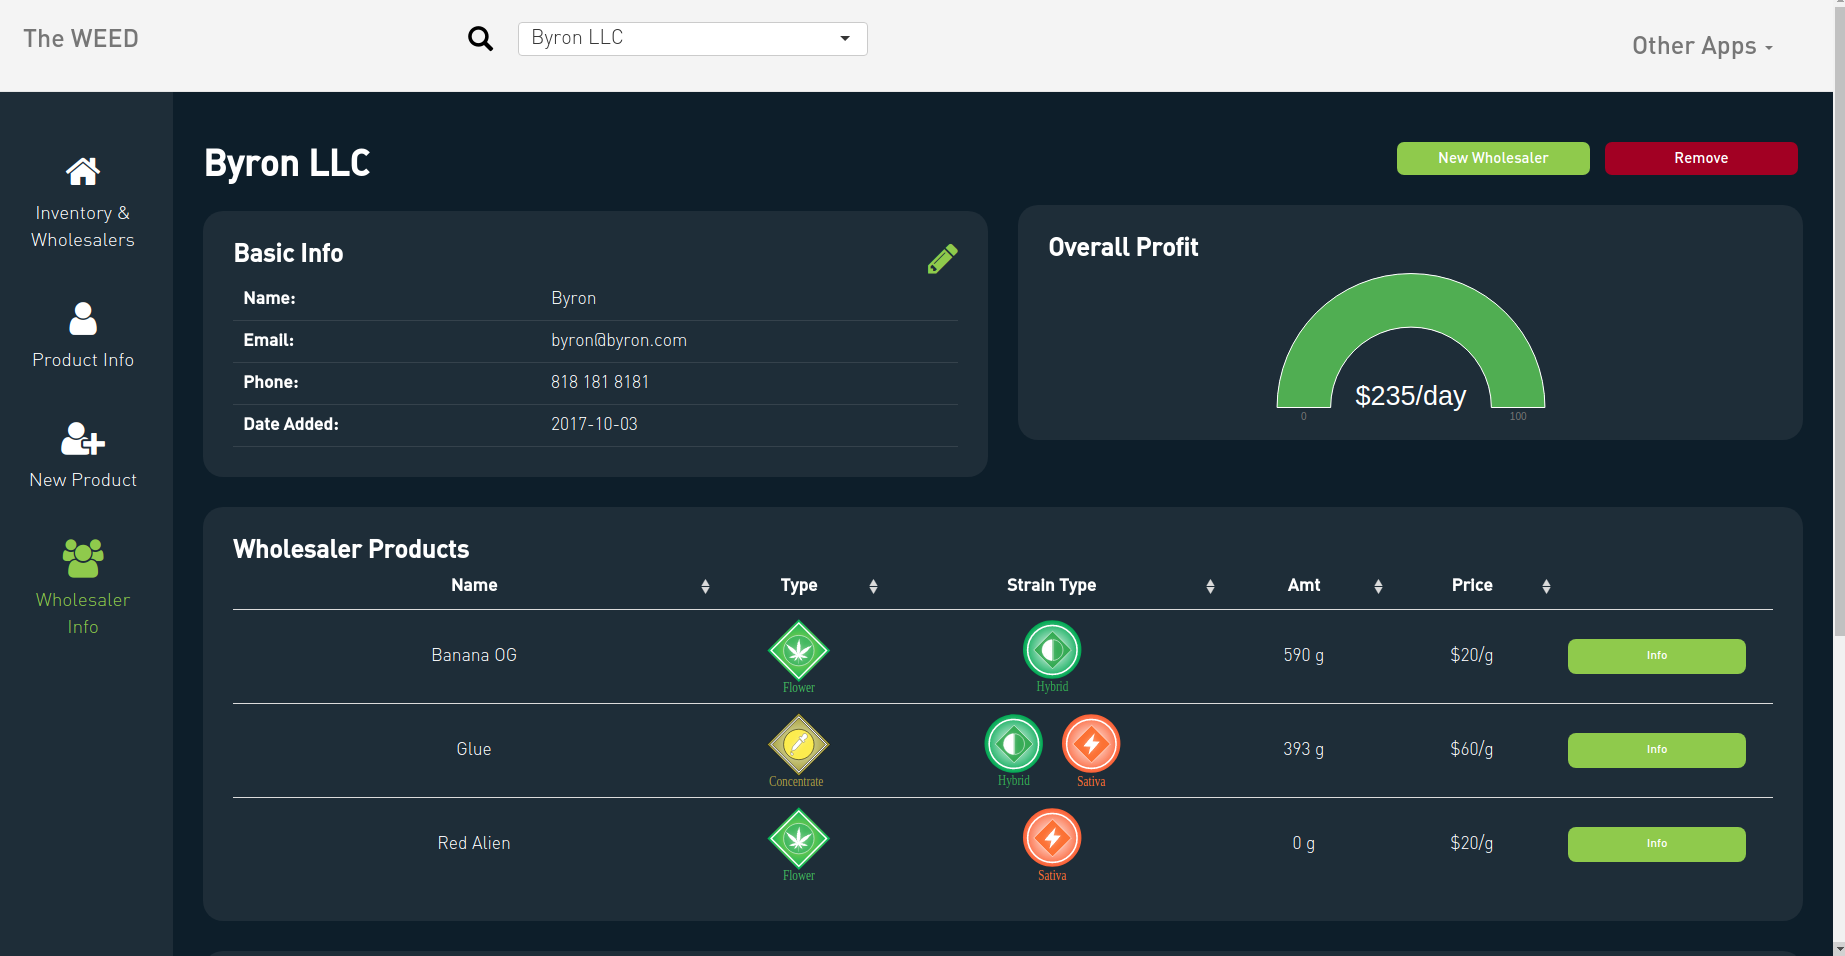
\includegraphics{images/wholesaler.png}
\caption{Wholesaler Info}
\end{figure}

Analytics about the wholesaler including daily sales, average daily
profit, and product type.

\begin{figure}
\centering
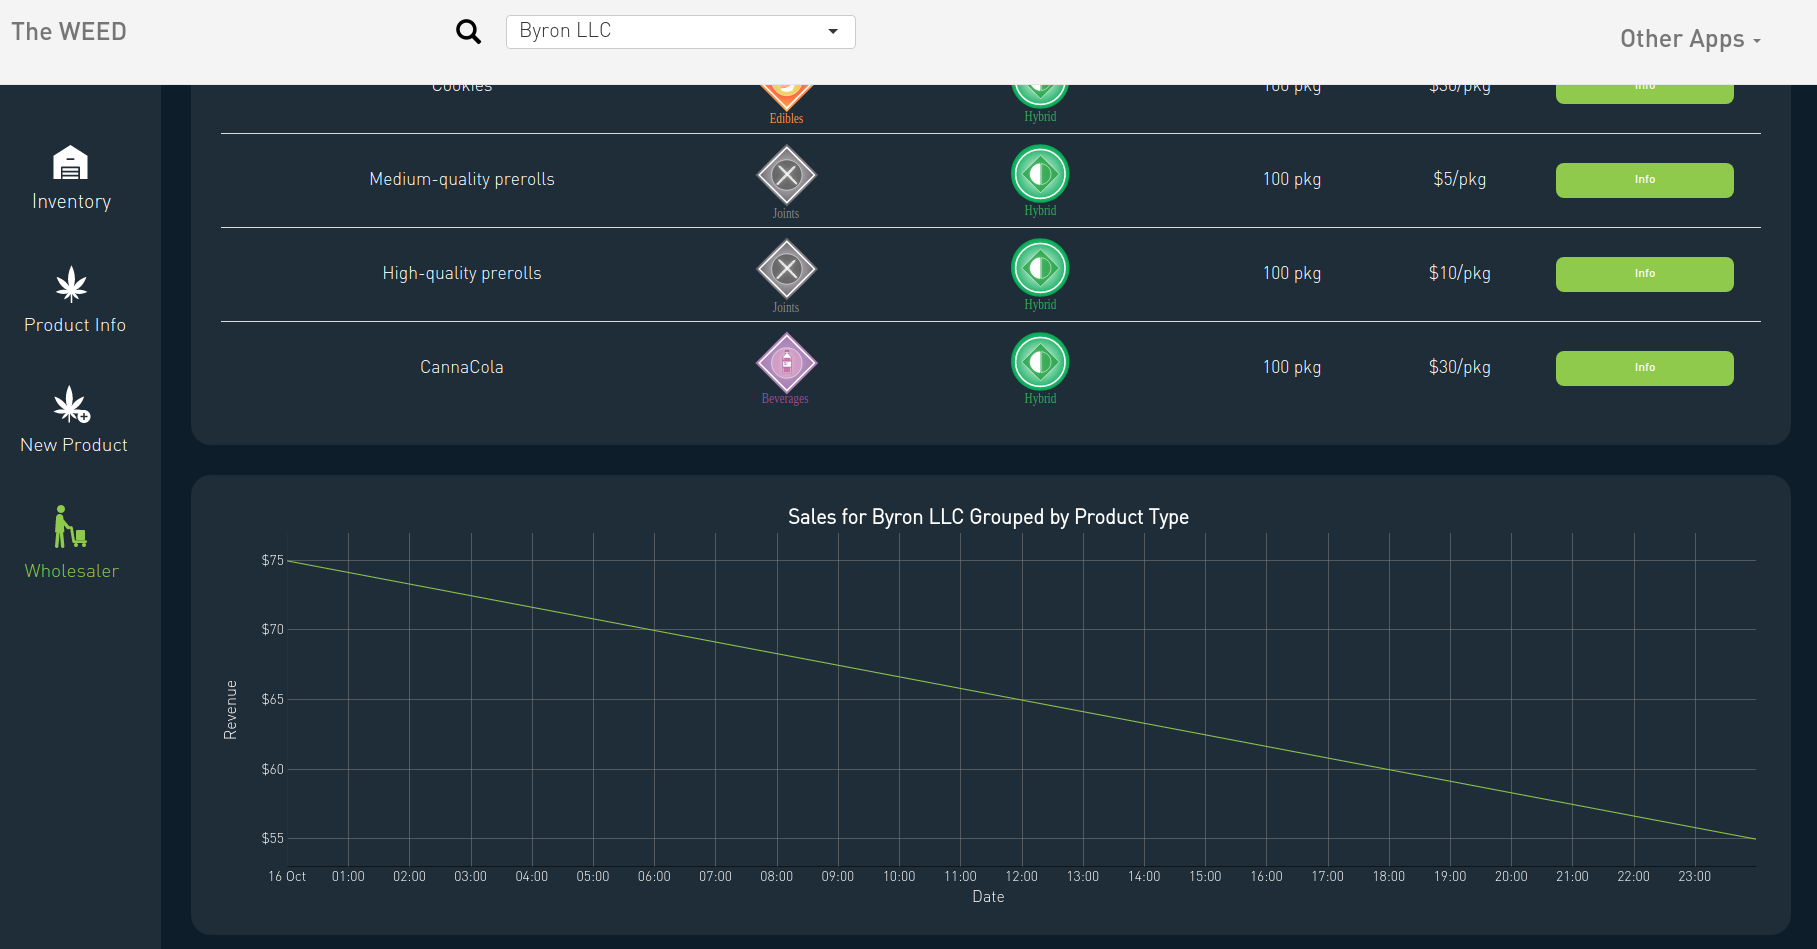
\includegraphics{images/wholesaler2.png}
\caption{Wholesaler Analytics}
\end{figure}

\section{New Wholesalers}\label{new-wholesalers}

New wholesalers can be added in either the new inventory page:

\begin{figure}
\centering
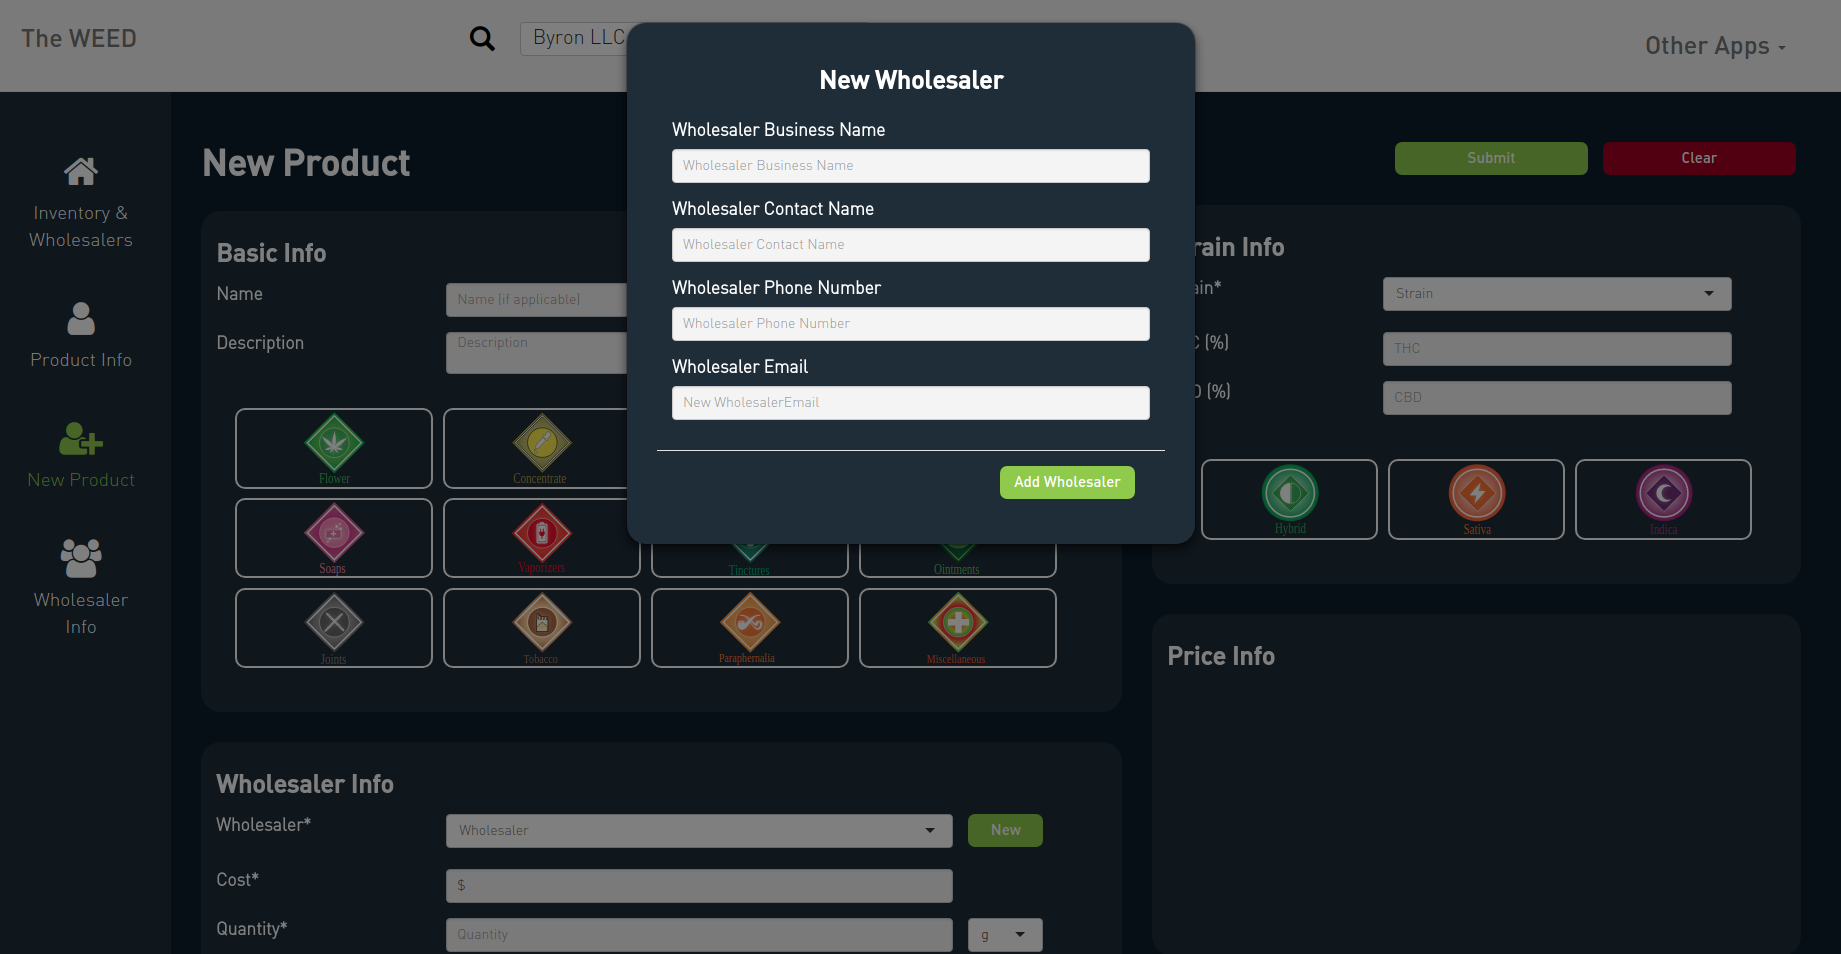
\includegraphics{images/newWholesaler.png}
\caption{New Wholesaler in New Inventory Page}
\end{figure}

Or in the wholesaler info page:

\begin{figure}
\centering
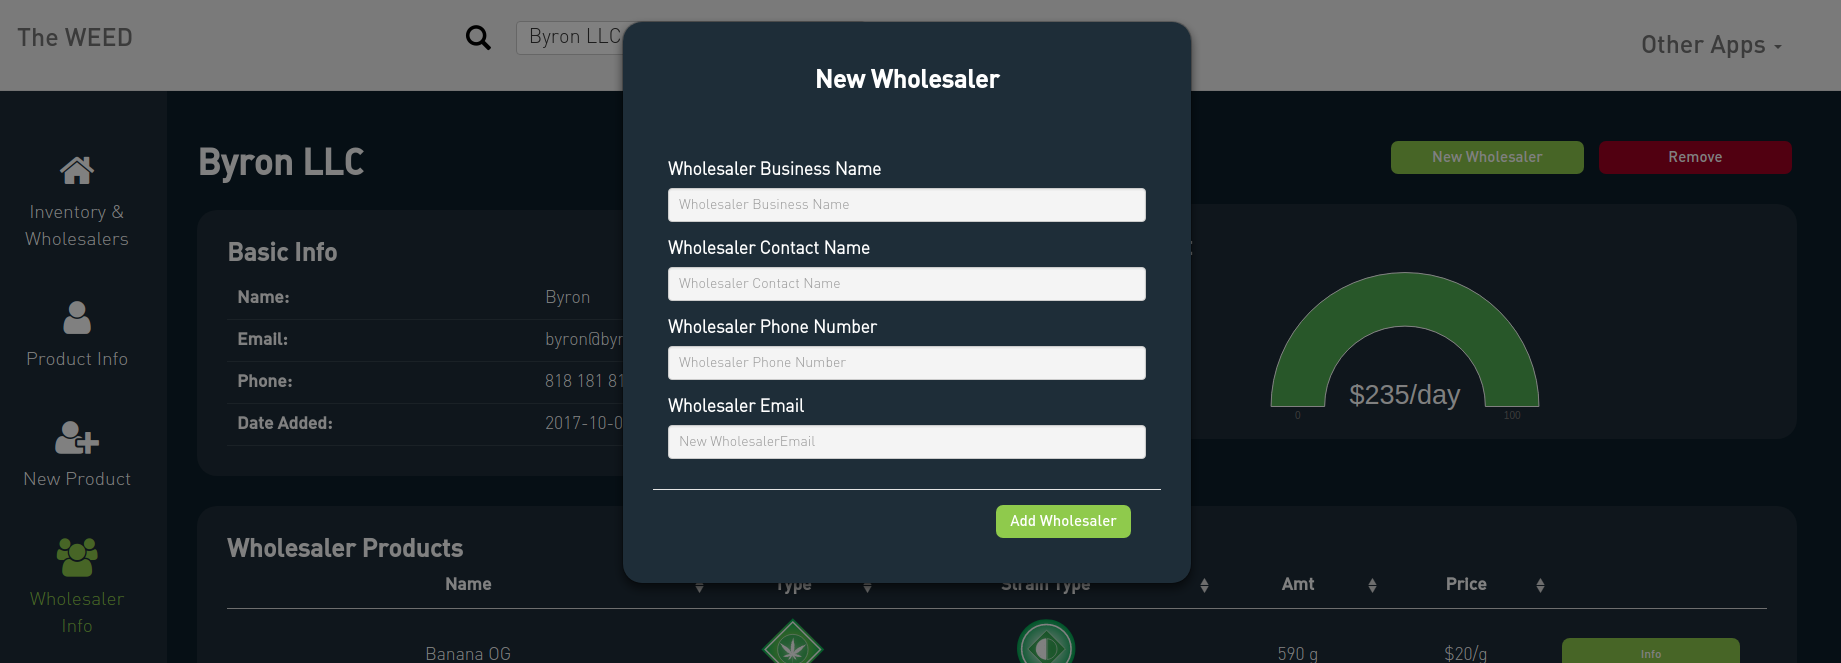
\includegraphics{images/newWholesaler2.png}
\caption{New Wholesaler in Wholesaler Info Page}
\end{figure}

\section{Labels}\label{labels}

Many dispensaries use labels and barcodes to organize their inventory.
There are two frameworks for using labels:

\begin{enumerate}
\def\labelenumi{\arabic{enumi}.}
\item
  Prepackage all products in advance
\item
  Keep products in larger container, and weigh out and package for each
  sale like a deli
\end{enumerate}

The second method is the most common, and it typically requires printing
one or two labels to place on the primary container. The first method
involves printing out a label for each prepackaged unit.

The product info page has a ``print label'' button, which provides the
user with a choice of either printing \emph{simple} labels for the
second method, or prepackaging the product.

\chapter{Point of Sales}\label{point-of-sales}

The point-of-sales application provides facilities for:

\begin{itemize}
\item
  Viewing patient info
\item
  Viewing current inventory
\item
  Processing transactions
\end{itemize}

\section{Patient Selection}\label{patient-selection}

To begin, you must select the current patient. The list of checked-in
patients is available in the navbar.

\begin{figure}
\centering
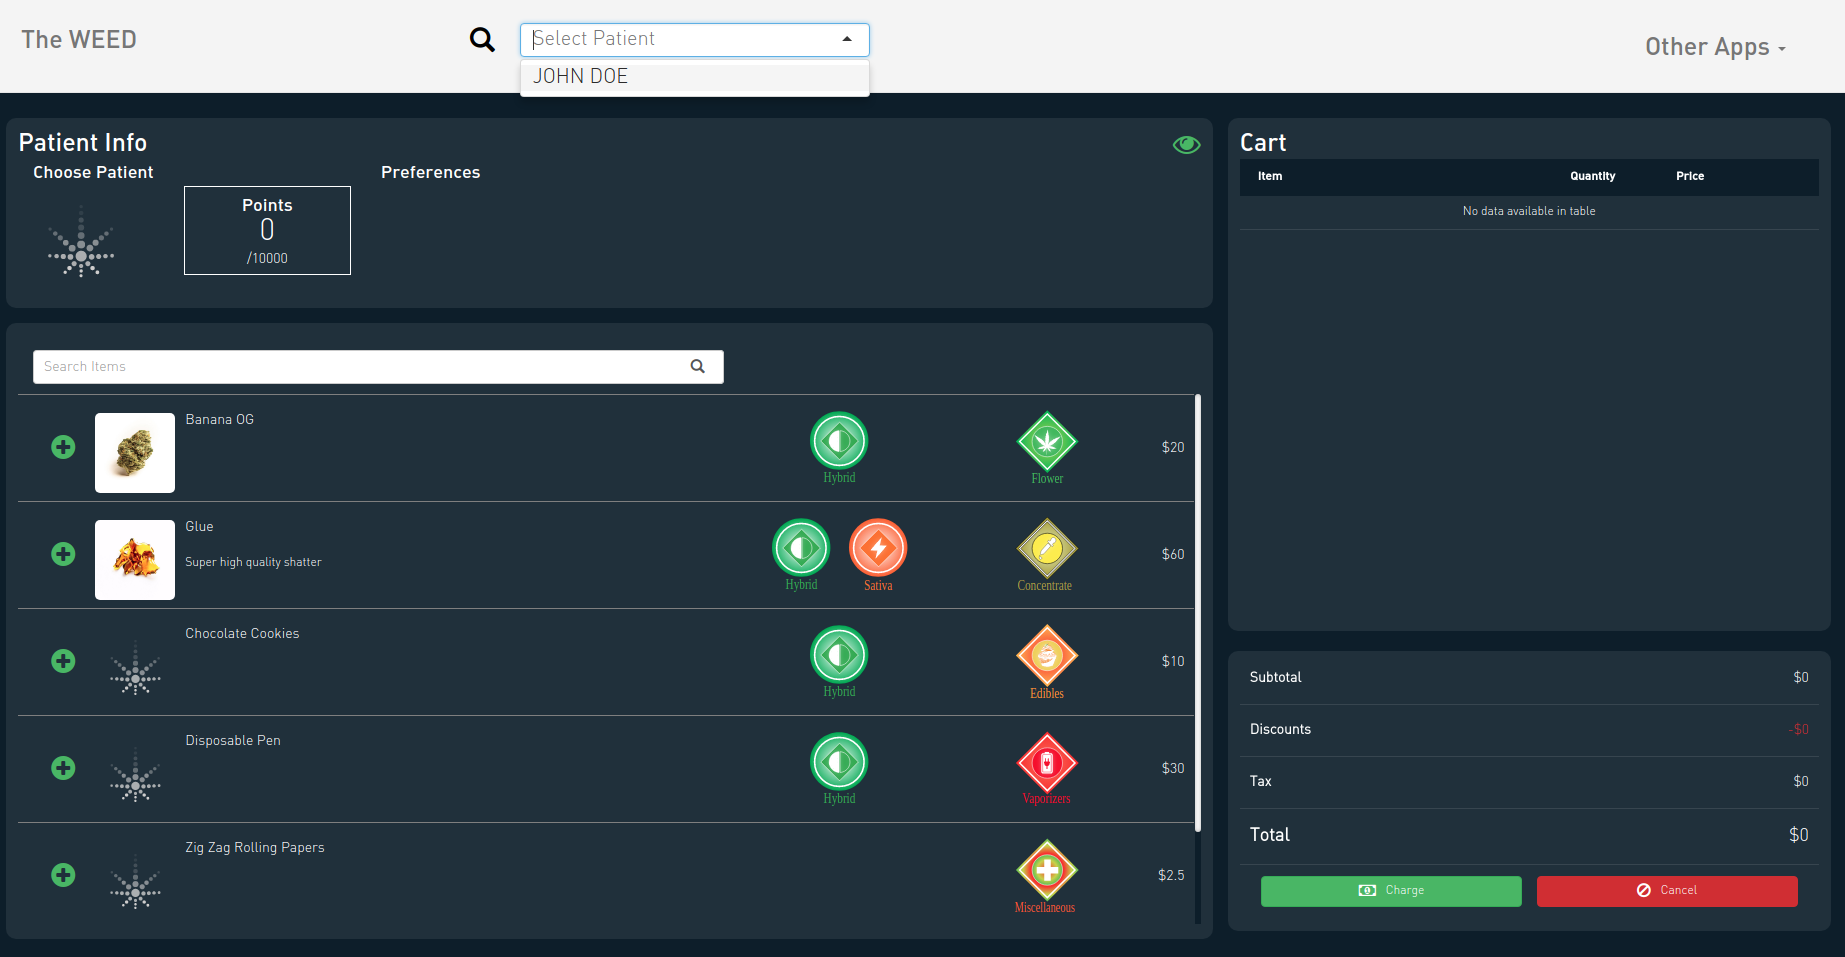
\includegraphics{images/P1.png}
\caption{Checked-in Patients can be selected in navbar}
\end{figure}

\section{Patient Info}\label{patient-info}

Once a patient is selected, their information appears at the top.

\begin{figure}
\centering
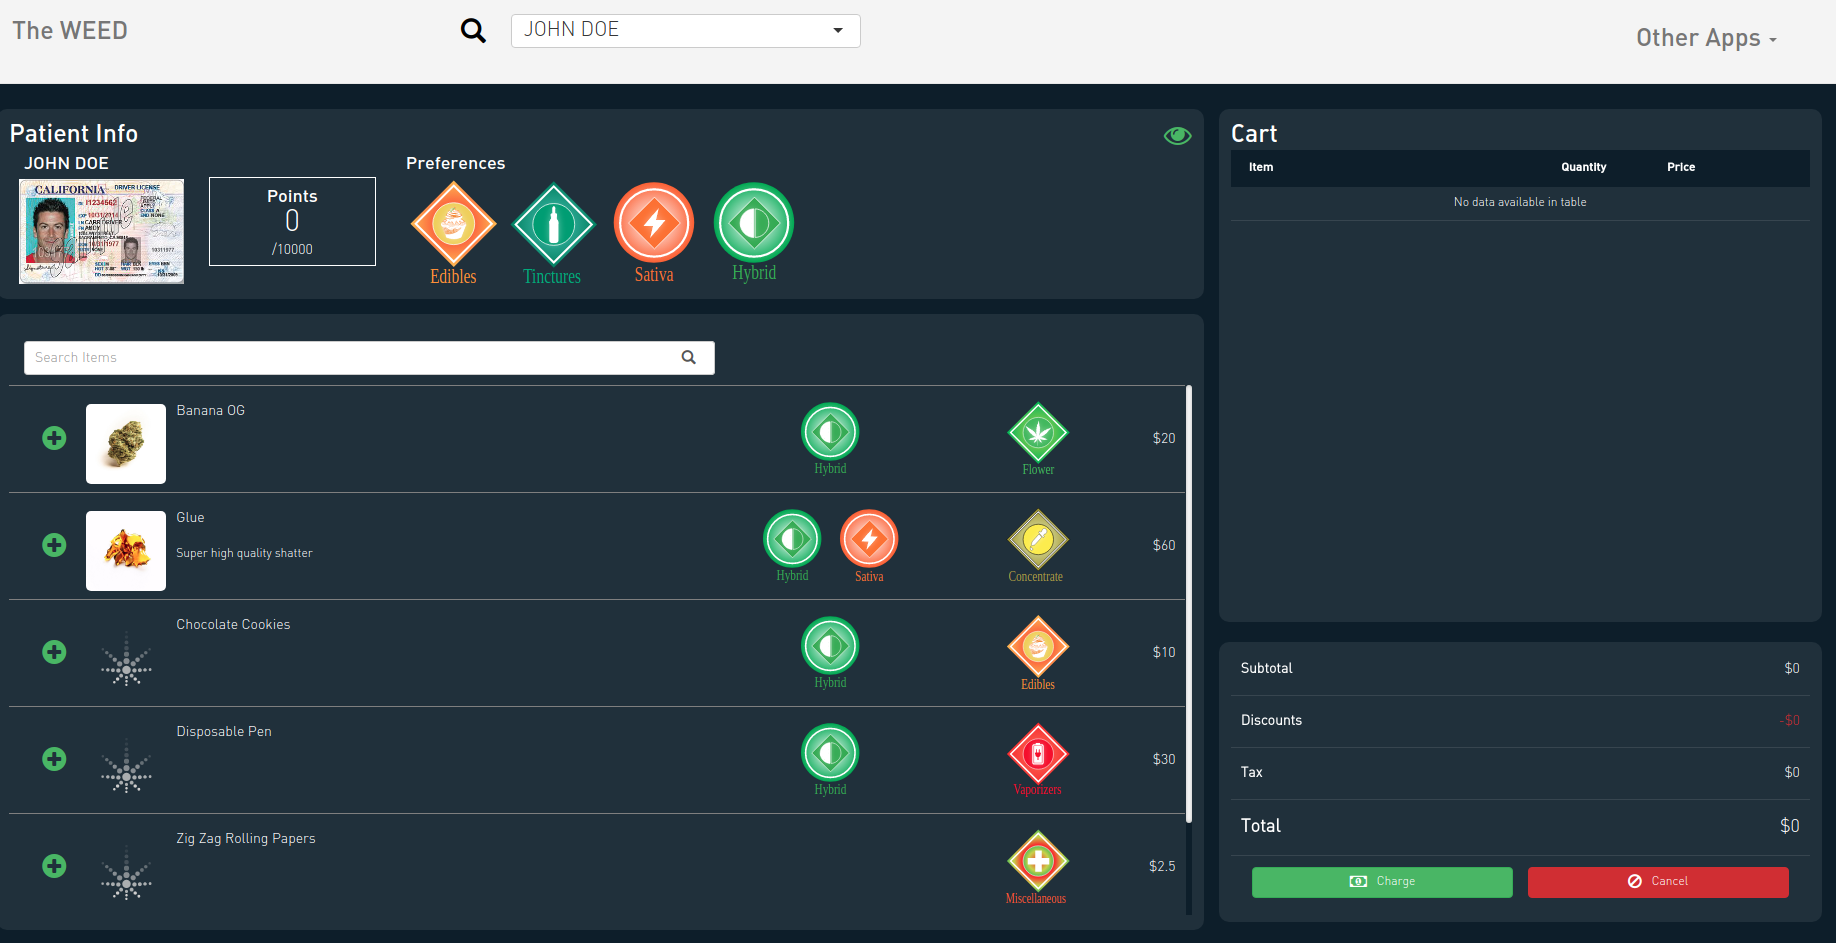
\includegraphics{images/P2.png}
\caption{Patient info appears once patient is selected}
\end{figure}

A more information about the patient is available by pressing the
eyeball to the top right of the patient information.

\begin{figure}
\centering
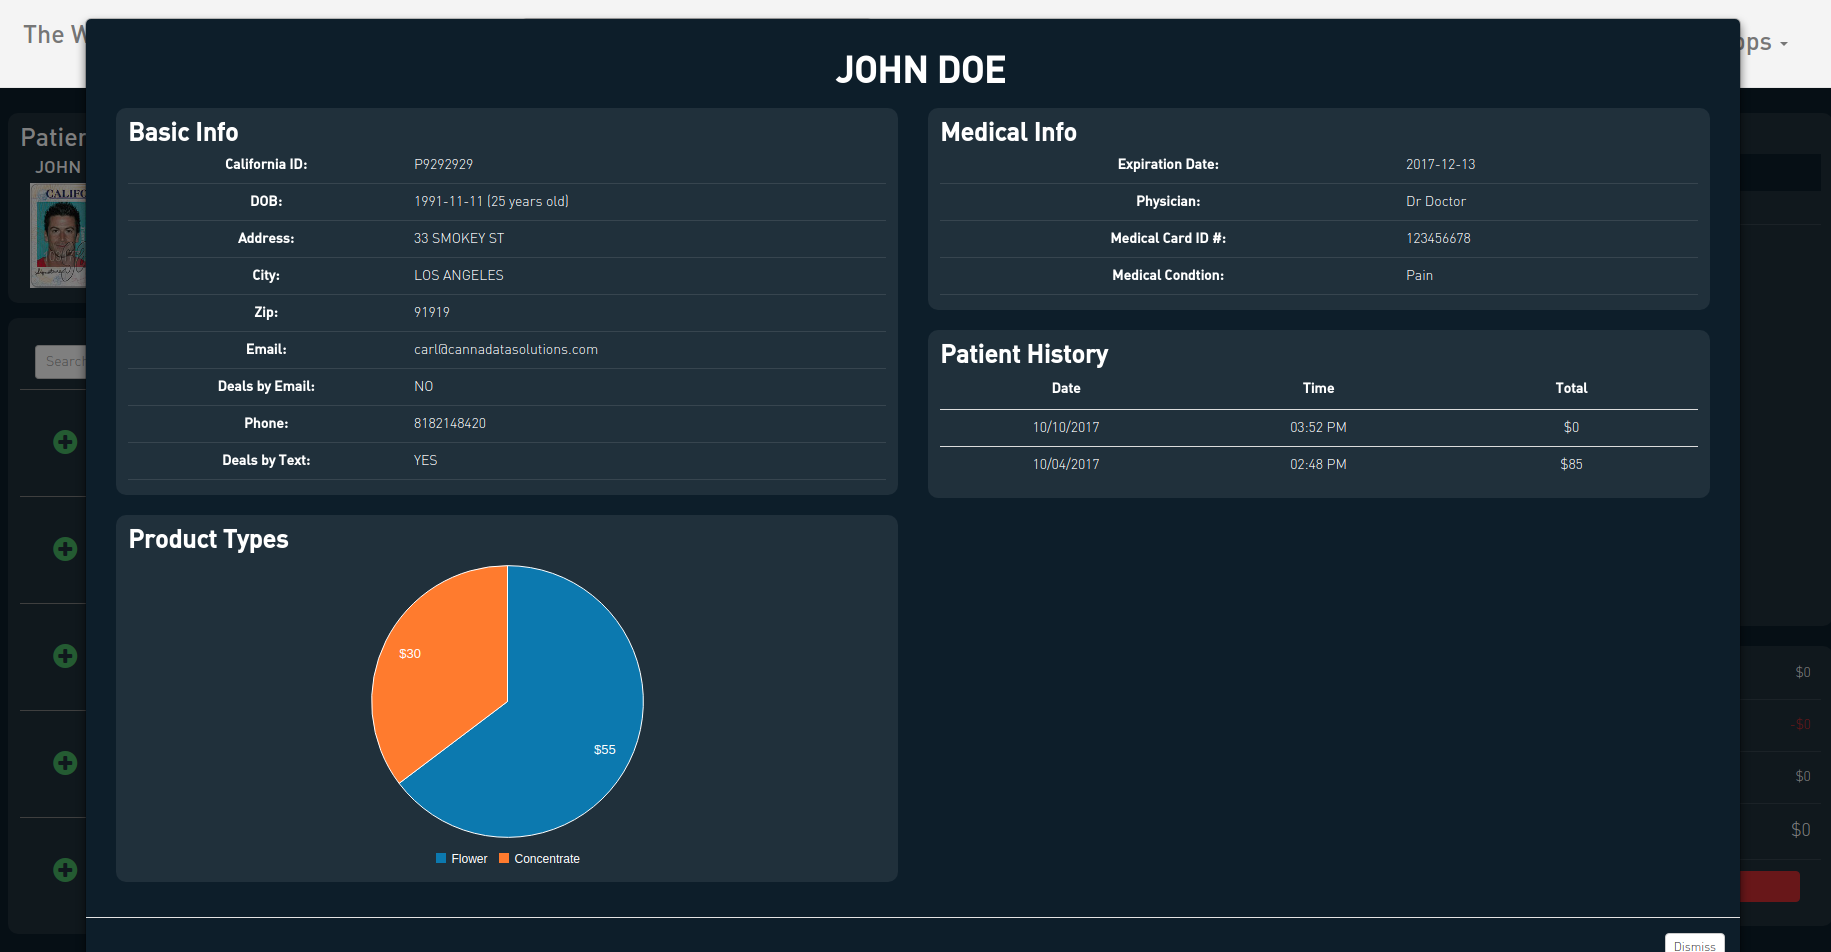
\includegraphics{images/P3.png}
\caption{Detailed info about the patient}
\end{figure}

This provides details about the patient's purchase history, as well as
the specifics of the patient's previous transactions.

\begin{figure}
\centering
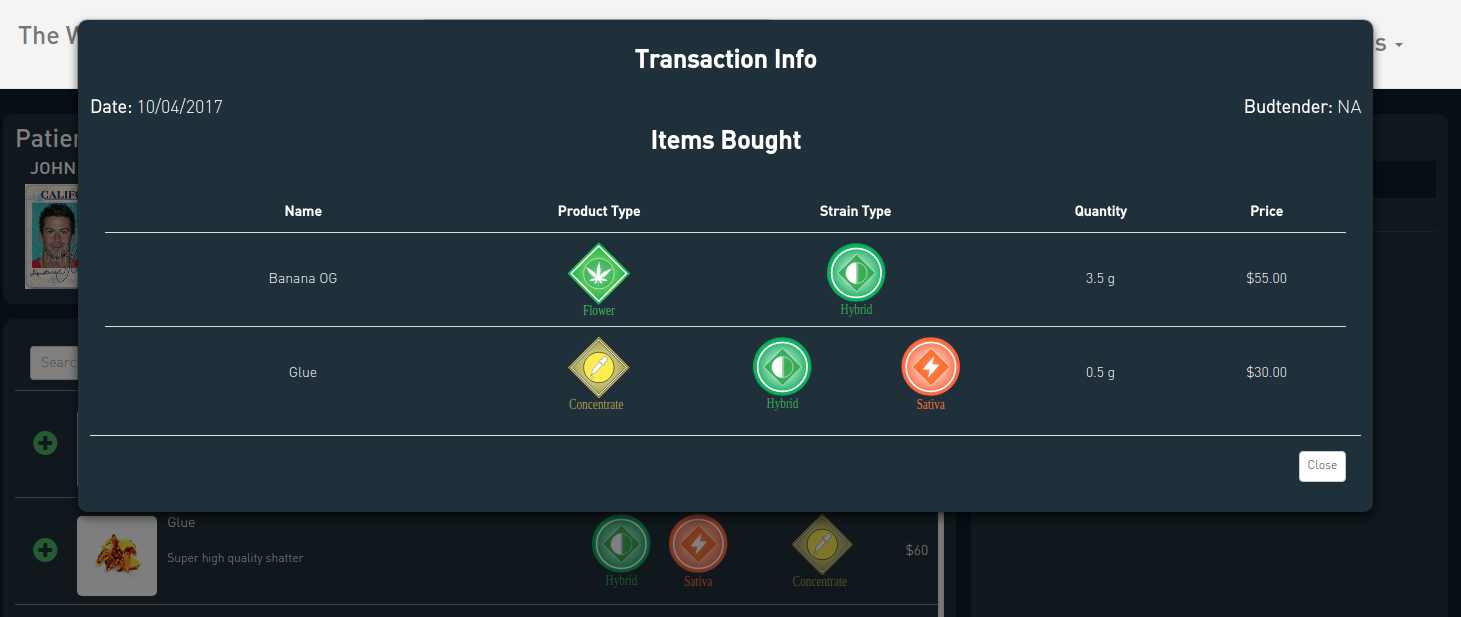
\includegraphics{images/P4.png}
\caption{Details from patient's previous transaction}
\end{figure}

\section{Sales}\label{sales}

There are two ways to add an item to the cart: by scanning a barcode, or
by selecting an item from the inventory table. When scanned, or
selected, the budtender is prompted to enter the exact information about
the sale: the quantity sold, and the price. The budtender also has the
option of applying a discount. (The discount info is automatically
populated if you register the coupon in the connect app i.e.~if you
create Wax Wednesday the discount will automaticaly populate for
concentrates on Wednesdays)

\begin{figure}
\centering
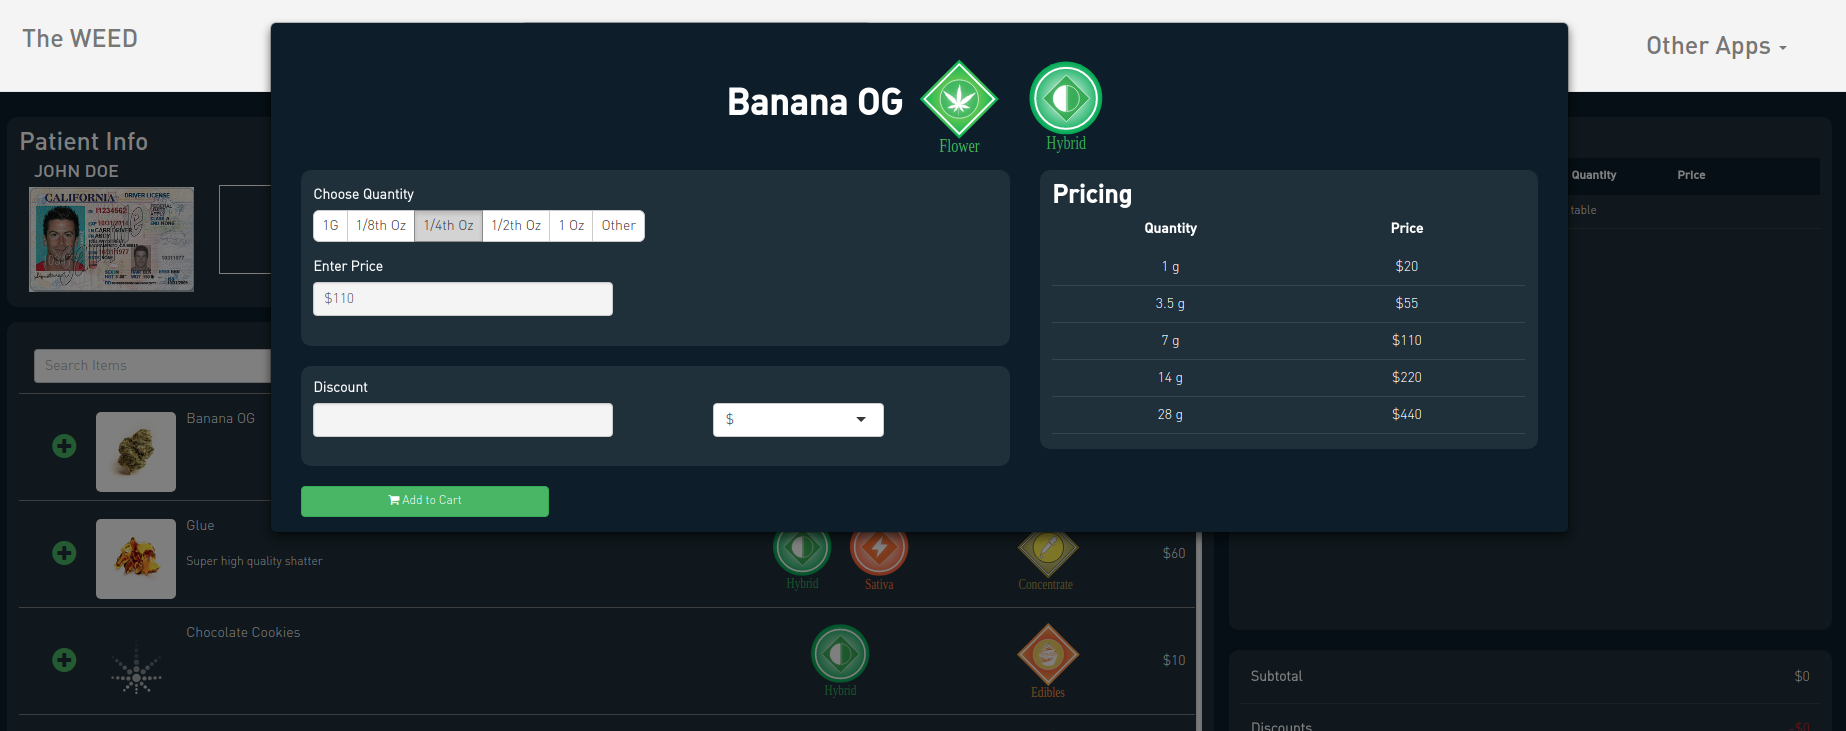
\includegraphics{images/P5.png}
\caption{Adding 1/4th of an Oz of Banana OG}
\end{figure}

You can enter arbitrary quantities, and it will determine the price.
Discounts can be added as either flat rates (i.e. \$10) or percentages.

\begin{figure}
\centering
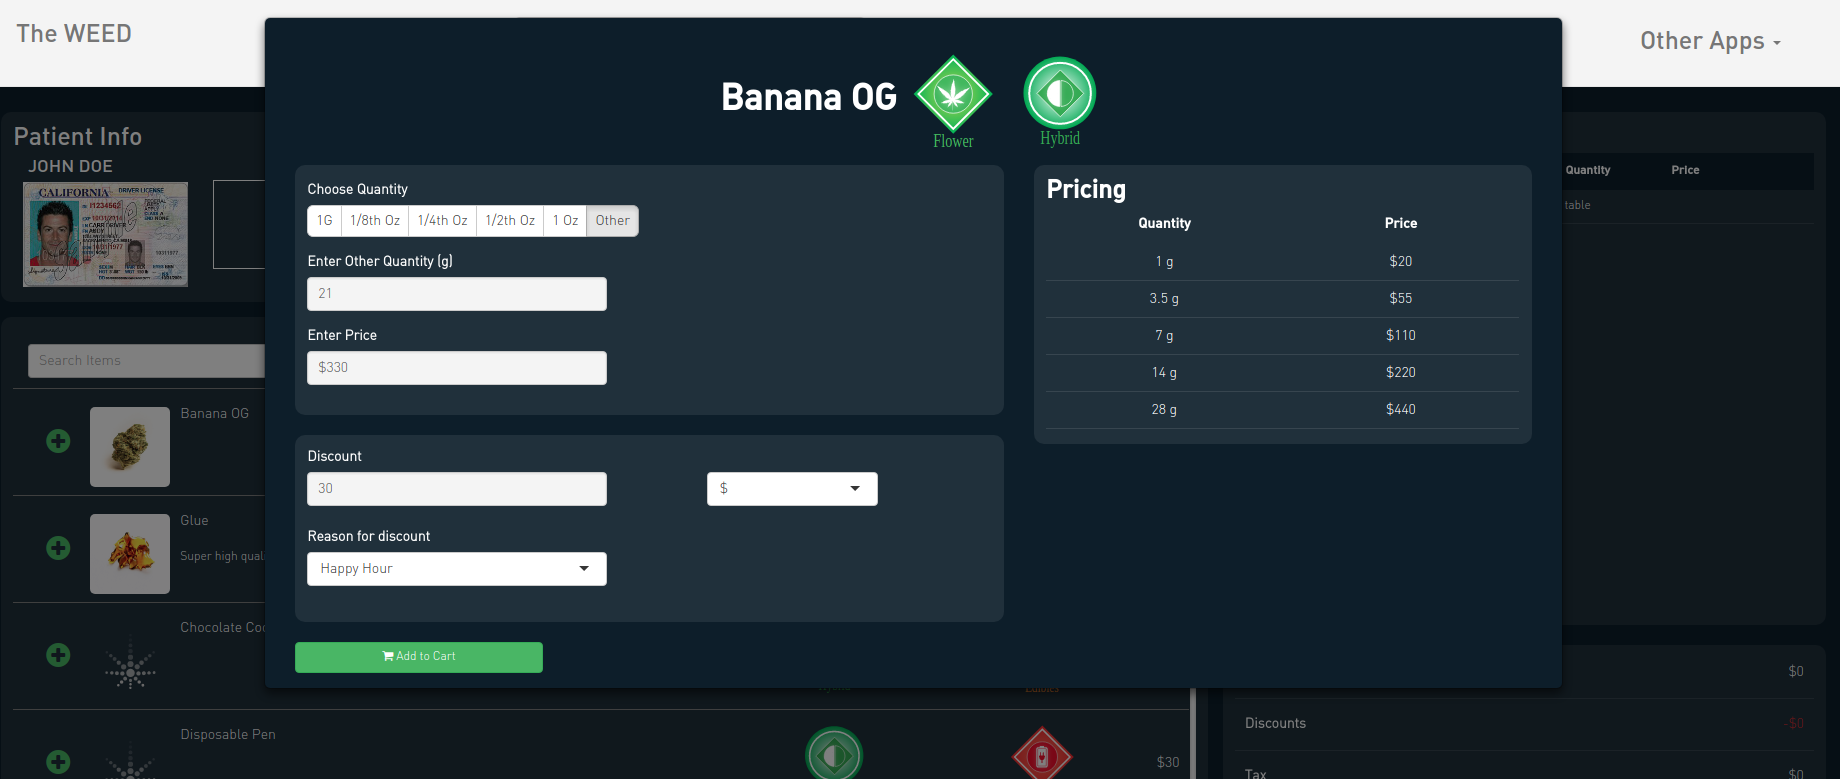
\includegraphics{images/P6.png}
\caption{Adding 21 grams of Banana OG, and applying Happy Hour discount}
\end{figure}

When added, the item appears in the cart. This information is not
session specific so you can leave the app, or process another patient's
transaction, and when you return the item will remain in the patient's
cart.

Item's in the cart can be edited by pressing the green pencil.

\begin{figure}
\centering
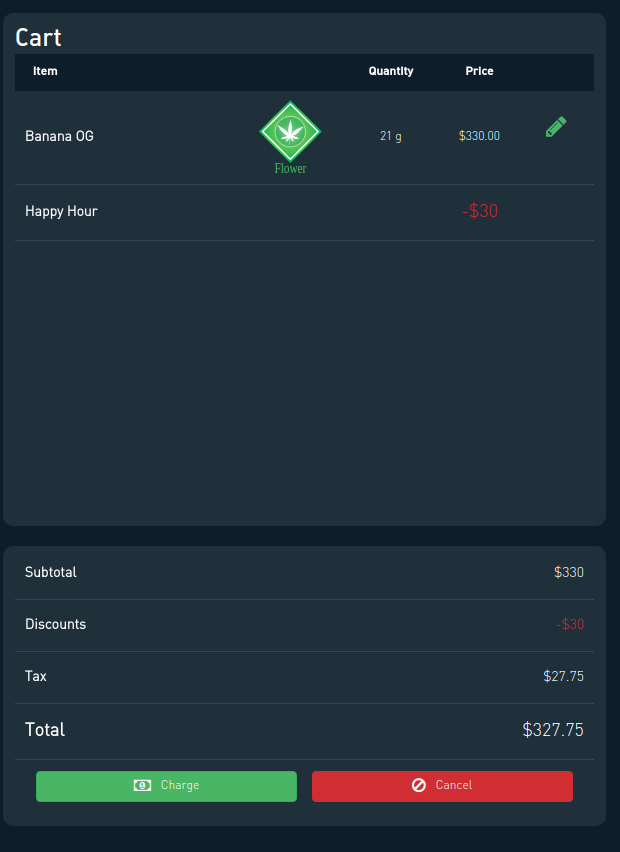
\includegraphics{images/P7.png}
\caption{Cart after adding Banana OG}
\end{figure}

\section{Searching}\label{searching}

When not using a barcode, it is often useful to search for the item you
are entering by name. You can also search for items by various
attributes like product type, strain name, strain type, and description.

\begin{figure}
\centering
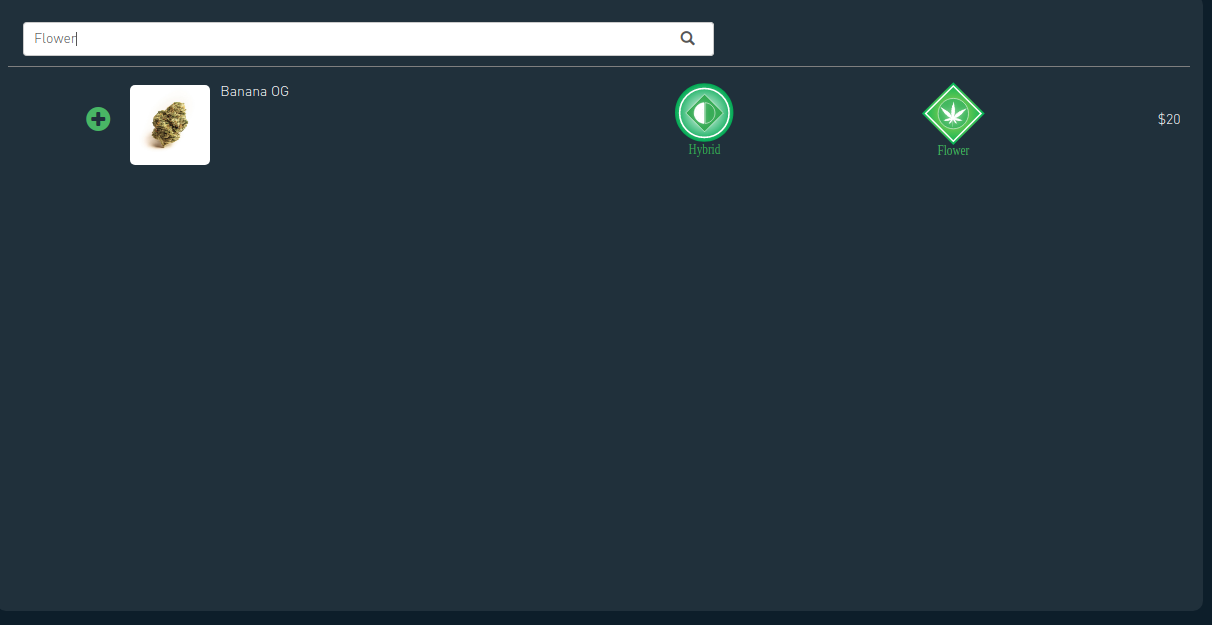
\includegraphics{images/P8.png}
\caption{Searching for flower in inventory}
\end{figure}

\section{Completing Transaction}\label{completing-transaction}

To complete the transaction press the green ``charge'' button on the
bottom right. This will prompt the budtender to enter the amount of cash
tendered. The budtender can enter the amount by either entering the
bills (i.e.~if budtender is handed two twenties and a ten they press
\$20, \$20, \$10) or by simply entering the amount (i.e.~press 5 then
0).

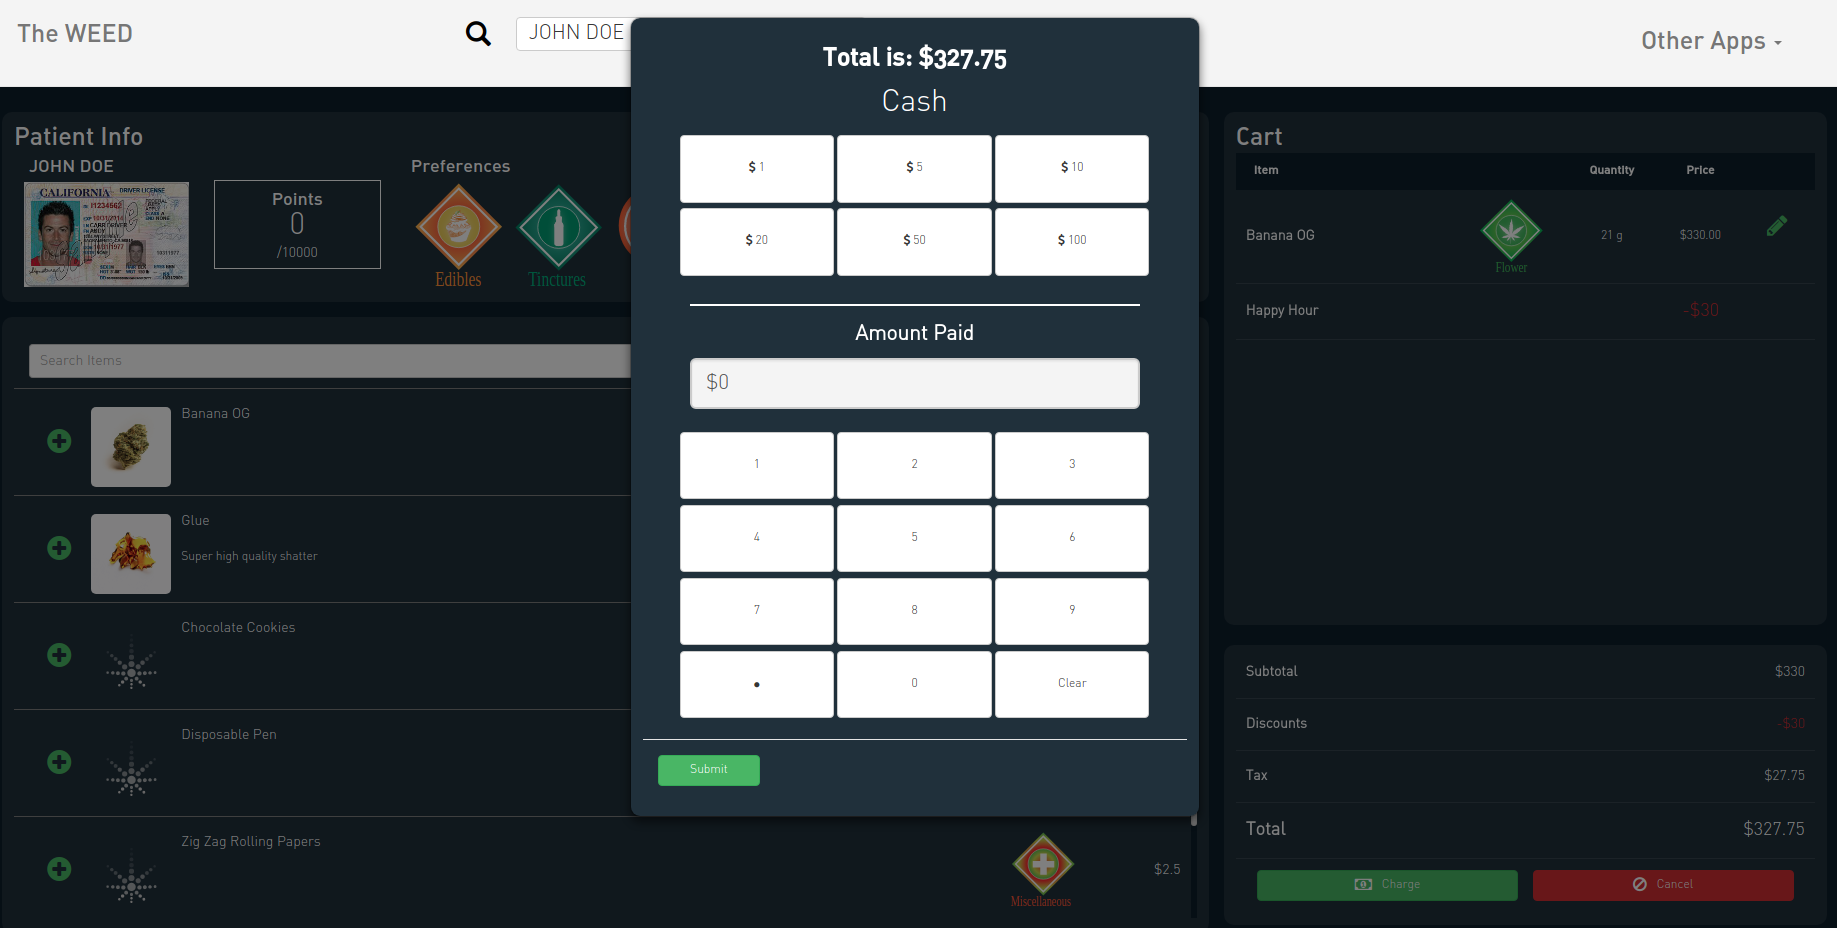
\includegraphics{images/P9.png} 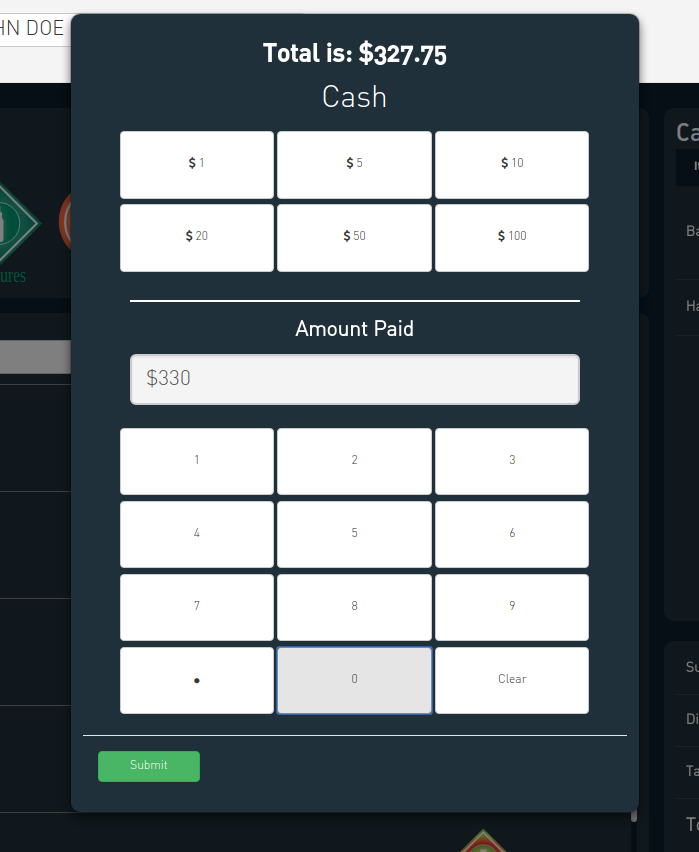
\includegraphics{images/P10.png}

Once the amount paid is submitted, the amount of change is returned, and
the transaction is complete.

\begin{figure}
\centering
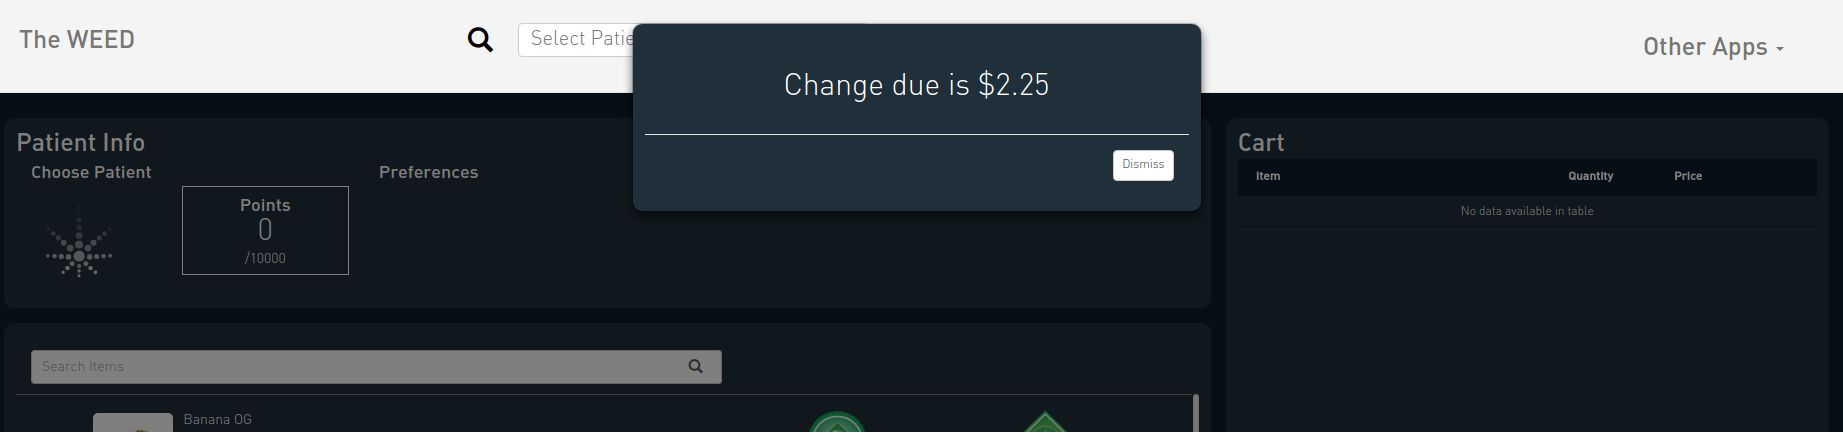
\includegraphics{images/P11.png}
\caption{After submitting amount paid, the amount of charge is given}
\end{figure}

\chapter{Connect}\label{connect}

\textbf{UNDER CONSTRUCTION}

Many dispensaries try to encourage patients to come to their store with
coupons, and targeted messages. The Connect Application provides
facilities for:

\begin{itemize}
\item
  Creating coupons/deals
\item
  Reaching out to patients via text, or email
\end{itemize}

\section{Coupons}\label{coupons}

\subsection{New Coupons}\label{new-coupons}

The required information for a new coupon is:

\begin{itemize}
\item
  A name
\item
  A discount (either a flat amount i.e. \$10, or a percentage i.e.~10\%)
\item
  A minimum (either a minimum total amount spent i.e. \$60, or a
  quantity i.e.~3.5 grams)
\item
  Which products the discount applies to. Options include:
\end{itemize}

\begin{enumerate}
\def\labelenumi{\arabic{enumi}.}
\tightlist
\item
  Total (i.e.~take 10\% off total bill)
\item
  All products of a certain type (i.e.~on Wax Wednesdays you discount
  \textbf{all} concentrates)
\item
  Specific products
\end{enumerate}

\begin{itemize}
\tightlist
\item
  Lastly you have to choose when the coupon is active
\end{itemize}

\begin{figure}
\centering
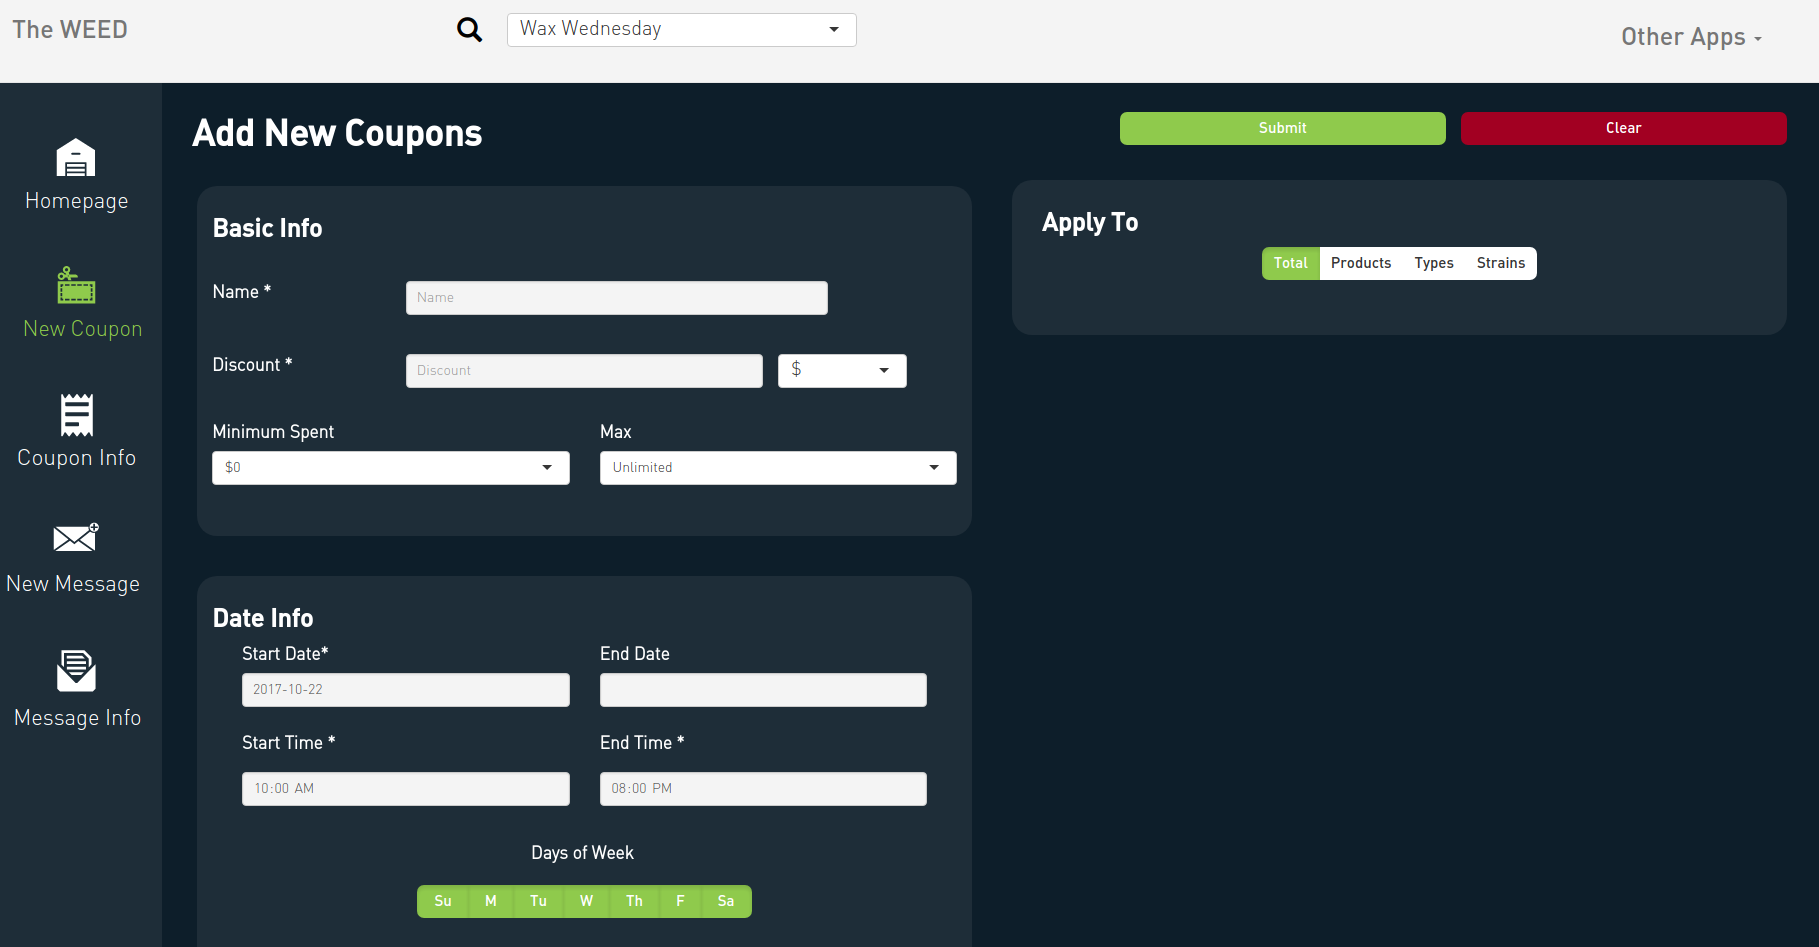
\includegraphics{images/C1.png}
\caption{Blank new coupon}
\end{figure}

\begin{figure}
\centering
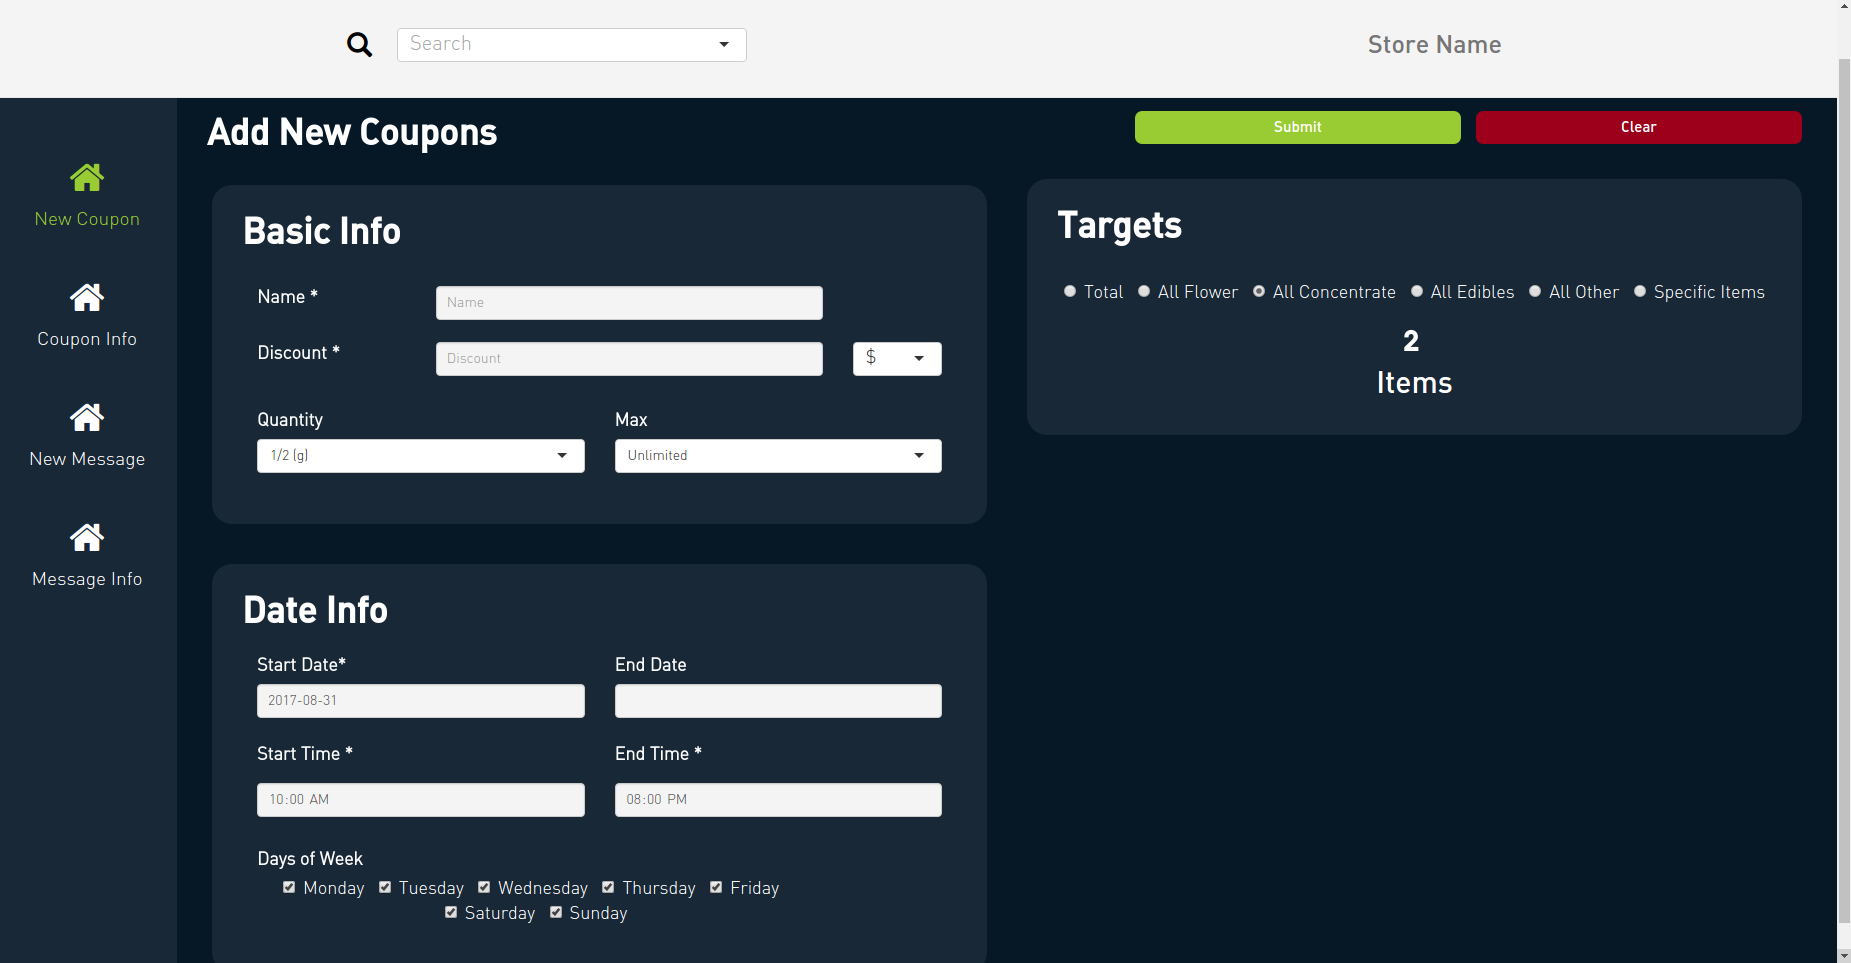
\includegraphics{images/C2.png}
\caption{Blank new coupon targeted at all concentrates}
\end{figure}

\begin{figure}
\centering
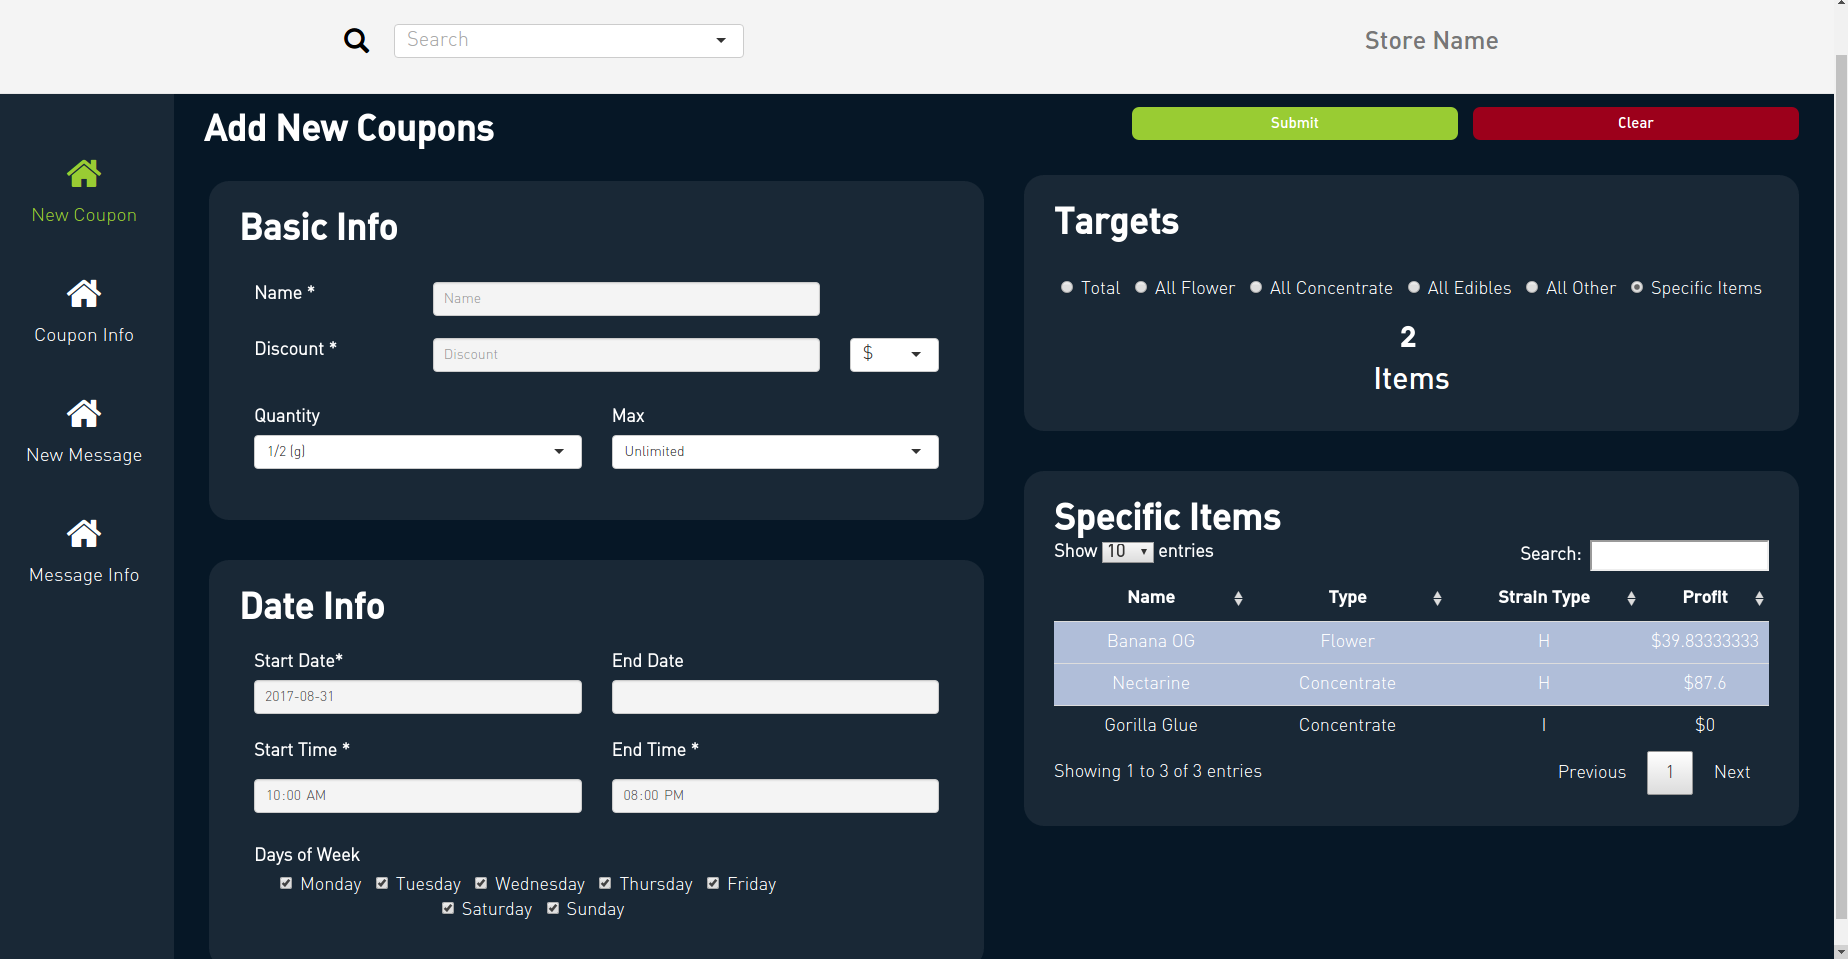
\includegraphics{images/C3.png}
\caption{Blank new coupon targeted at specific items}
\end{figure}

\subsection{Coupon Info}\label{coupon-info}

You can view information about existing coupons by selecting them in the
search box in the top. The coupon info page provides basic information
that can be edited as well as a list of current inventory that is
discounted when the coupon is active. There is a graph of daily sales
for the discounted products, which enables you to see if the coupon
created a positive bump.

\begin{figure}
\centering
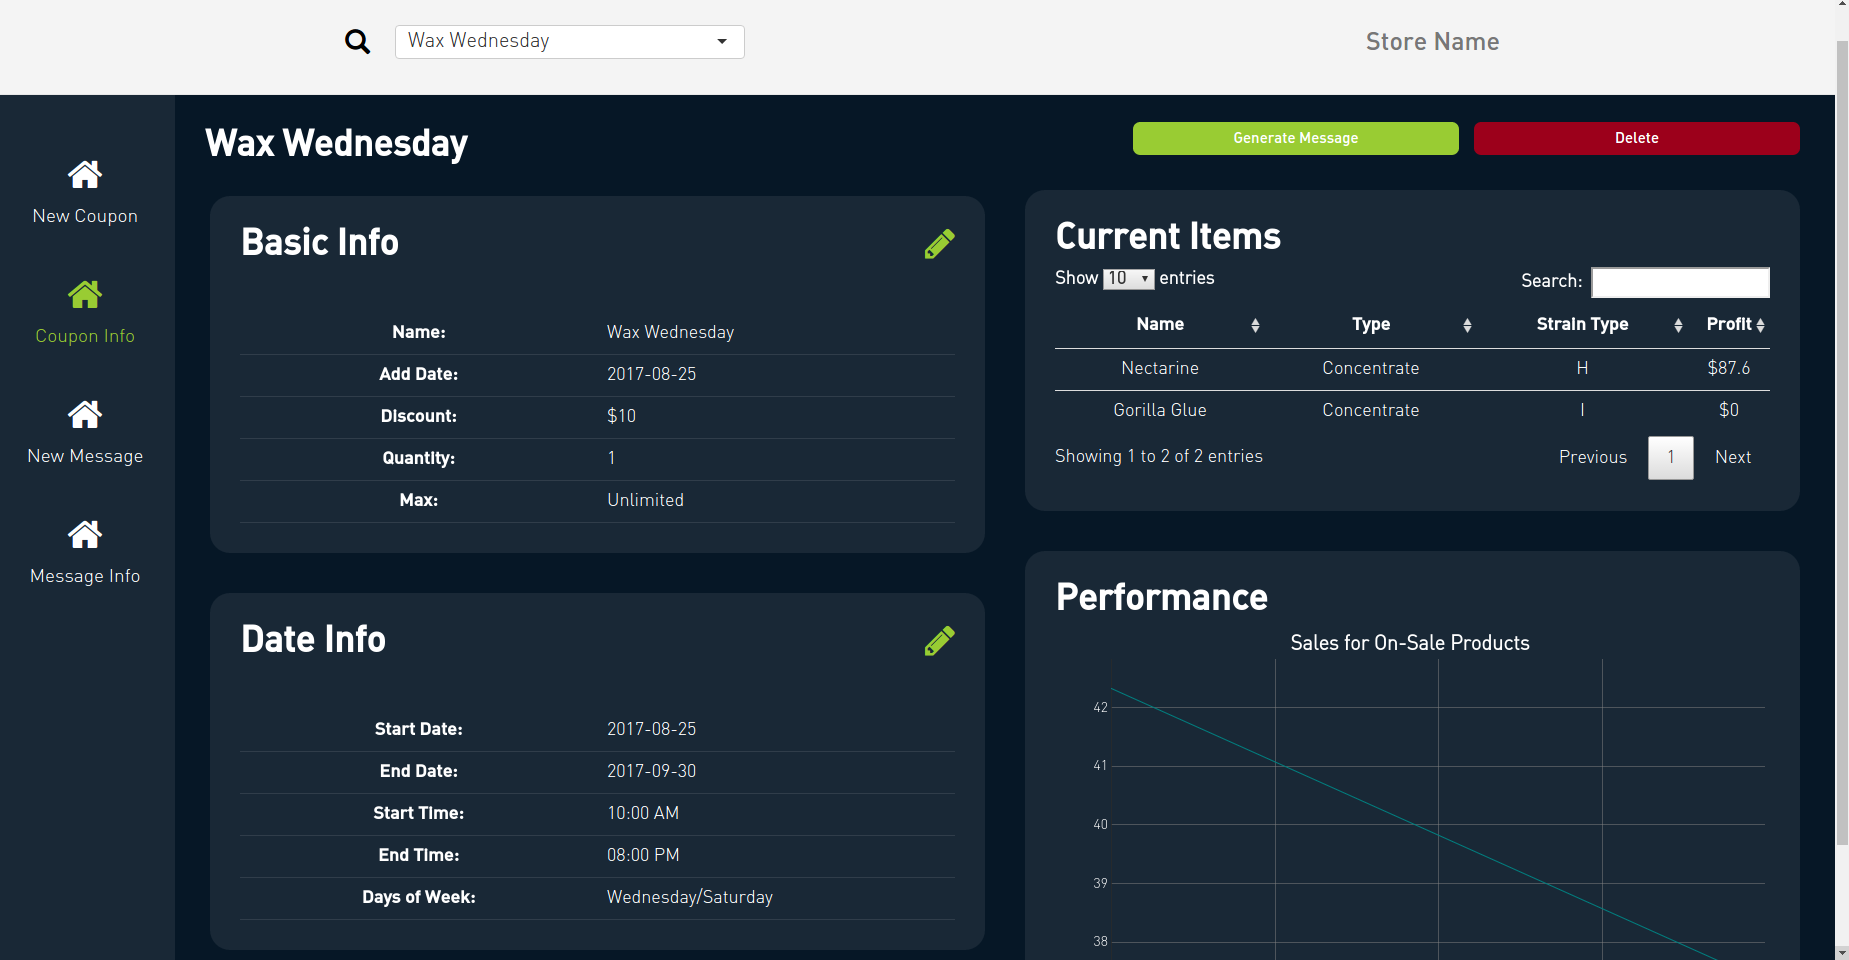
\includegraphics{images/C4.png}
\caption{Info for Wax Wednesday}
\end{figure}

\section{Messages}\label{messages}

\subsection{New Messages}\label{new-messages}

To send a new message out to patients you are required to enter:

\begin{itemize}
\item
  A name
\item
  Message type (text or email)
\item
  Audience (based on patient preferences)
\item
  The message
\item
  If you send an email a subject is required
\end{itemize}

\begin{figure}
\centering
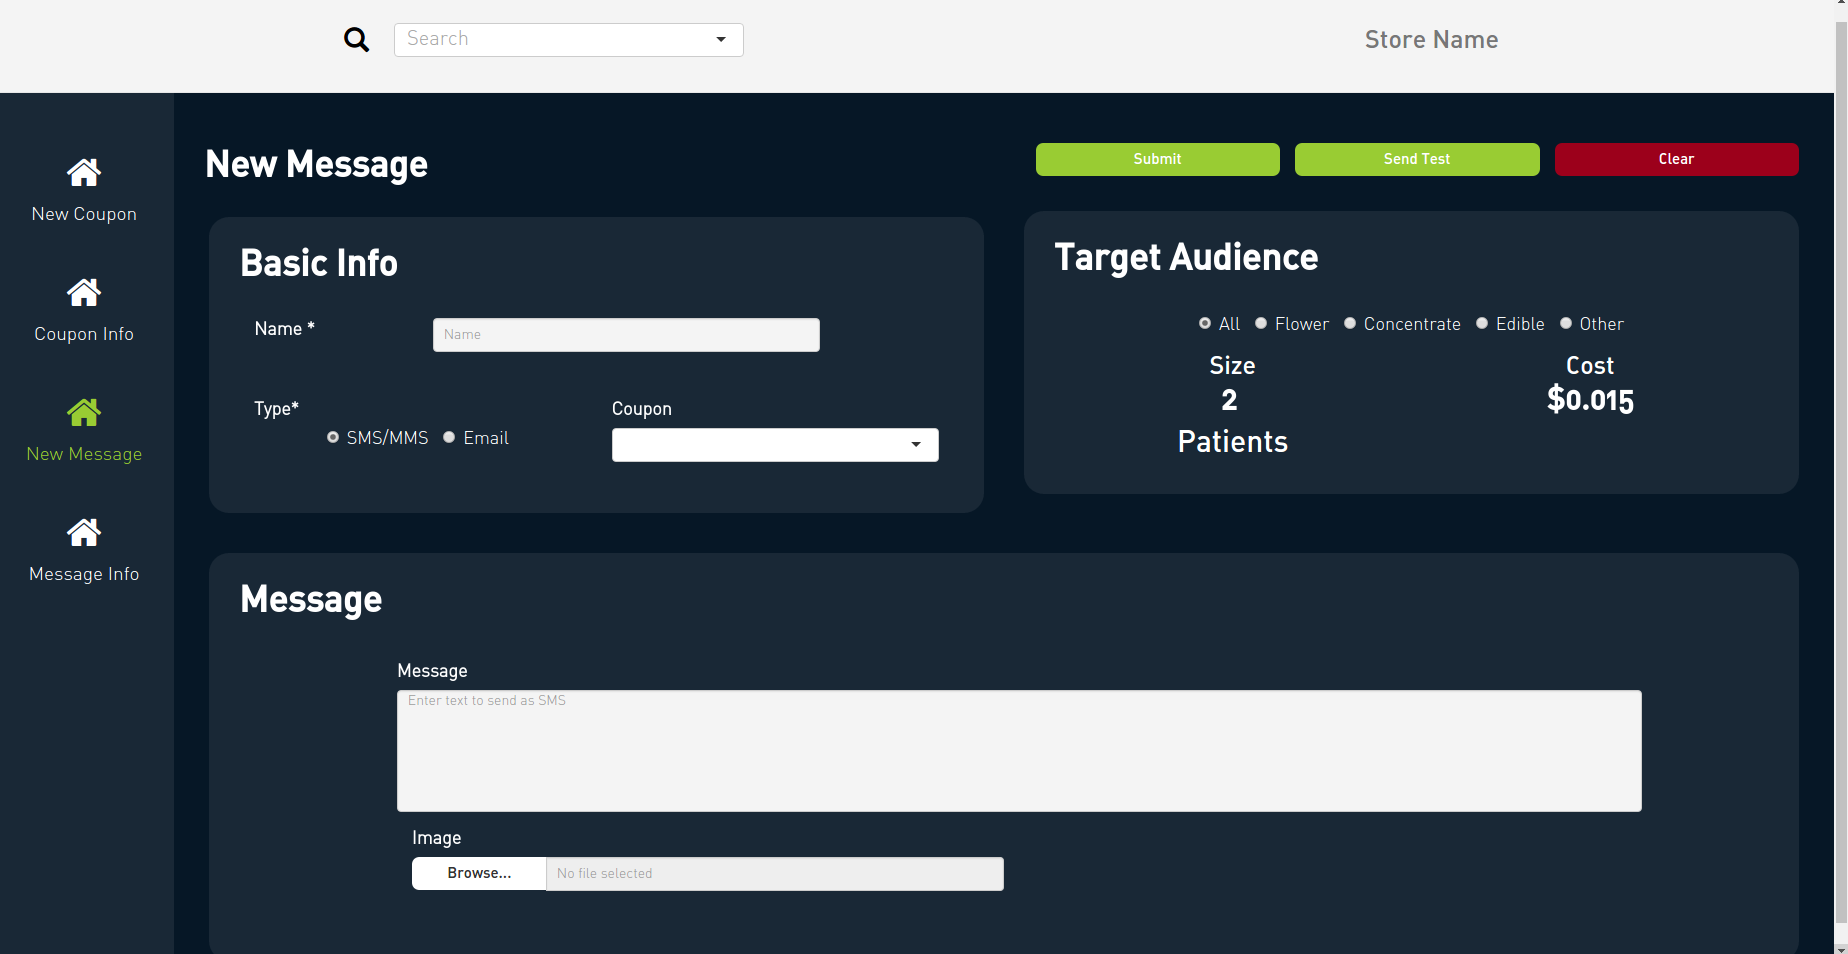
\includegraphics{images/C5.png}
\caption{New Text Message}
\end{figure}

\begin{figure}
\centering
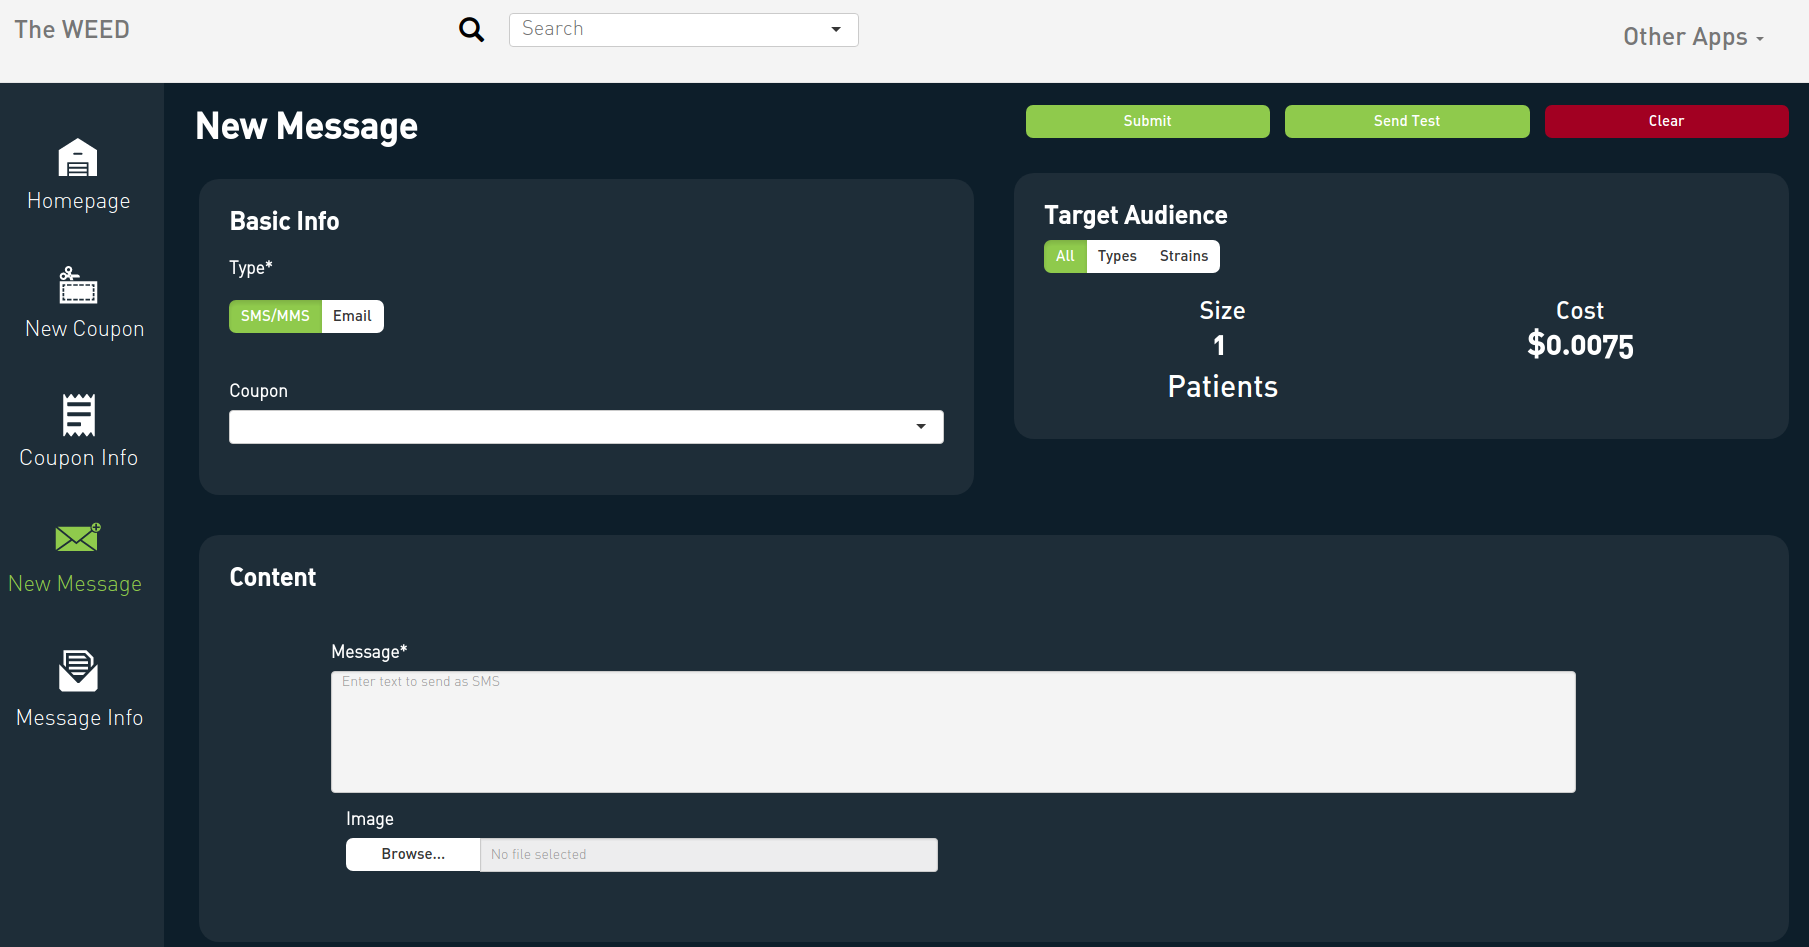
\includegraphics{images/C6.png}
\caption{New Email}
\end{figure}

\subsection{Message Info}\label{message-info}

You can review the info about past messages by selected the message in
the search box at the top. This will give you basic info about the
message like when it was sent, to whom, and its content. There is also a
graph of daily sales of the patients who were messaged, which makes it
easy to check whether the message led to a noticable increase in sales.

\begin{figure}
\centering
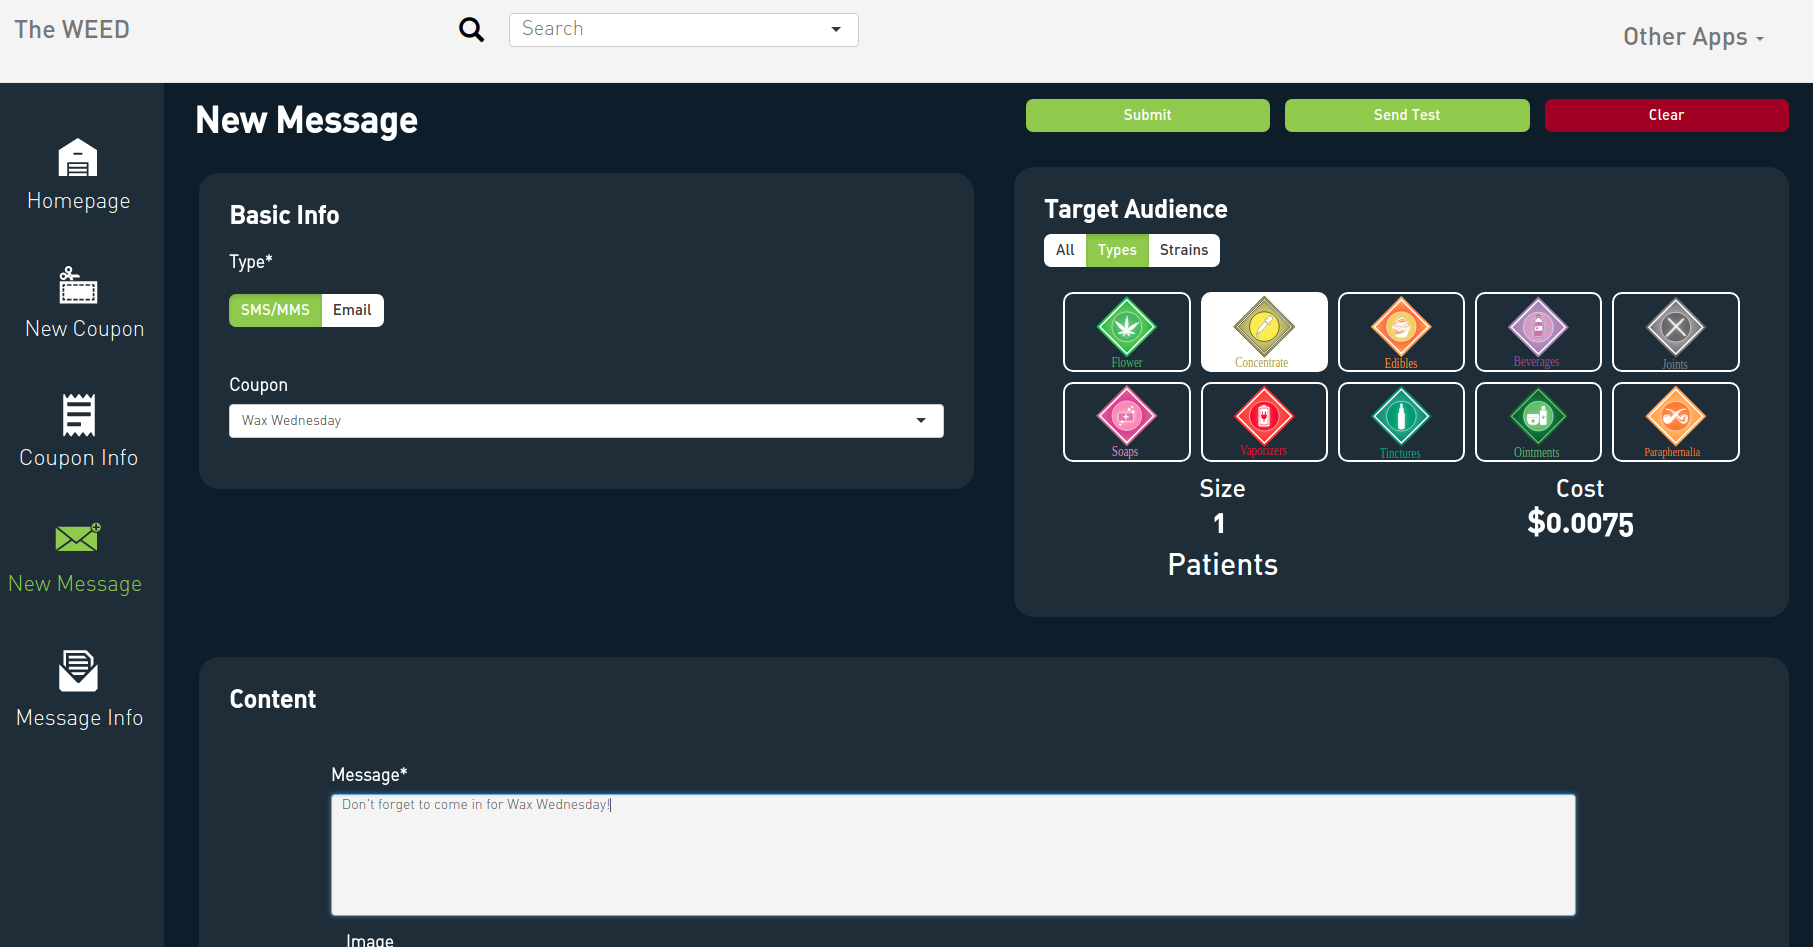
\includegraphics{images/C7.png}
\caption{Message Info for Wax Alert}
\end{figure}


\end{document}
